% =====================================================================
%  CSE 401: Numerical Analysis, Simulation and Modeling -- Assignment
%  Topic 3: Gradient Methods
%  Roll: 2105032
%  Build:  pdflatex 2105032 ; bibtex 2105032 ; pdflatex 2105032 ; pdflatex 2105032
%          (or: latexmk -pdf 2105032.tex). No shell-escape needed.
% =====================================================================
\documentclass[aspectratio=169, 11pt]{beamer}
% =====================================================================
%  preamble.tex -- packages, theme, colours, macros
%  Gradient Methods (CSE 401), Nawriz Ahmed Turjo, Roll 2105032
%  Engine: pdfLaTeX, no shell-escape required.
%
%  Visual system (built on Metropolis):
%    * light "paper" content slides, dark navy only for the title slide and
%      big-statement slides;
%    * three colours with fixed jobs: navy = structure, orange = attention,
%      teal = answers and key results;
%    * white frame header with a section label and an orange progress rule;
%    * numbered section dividers with a "you are here" stop strip;
%    * left-accent boxes; Part B frames carry a navy strip with the problem id.
% =====================================================================

% ---------- theme ----------
\usetheme[progressbar=none, numbering=fraction, block=fill]{metropolis}
\setbeamertemplate{frame footer}{Gradient Methods \quad|\quad Nawriz Ahmed Turjo \quad|\quad 2105032}
\setbeamersize{text margin left=0.9cm, text margin right=0.9cm}

% ---------- encoding / fonts ----------
\usepackage[T1]{fontenc}
\usepackage[utf8]{inputenc}
\usepackage[sfdefault, lining, scaled=0.92]{FiraSans}   % text
\usepackage[scaled=0.86]{FiraMono}                       % code
\renewcommand*\familydefault{\sfdefault}

% ---------- mathematics ----------
\usepackage{amsmath, amsthm, mathtools}
\usefonttheme{professionalfonts}                         % let the packages below set the maths fonts
\usepackage{newtxsf}                                     % matching sans-serif maths (after amsmath)
\usepackage{nicefrac}

% ---------- graphics / tables ----------
\usepackage{graphicx}
\graphicspath{{figures/generated/}{figures/tikz/}}
\usepackage{booktabs, array, multirow, makecell}
\usepackage{tikz}
\usetikzlibrary{arrows.meta, calc, positioning, shapes.geometric, shadows, fadings,
                decorations.pathmorphing, decorations.pathreplacing, patterns, backgrounds}
\usepackage{xcolor}

% ---------- boxes ----------
\usepackage[most]{tcolorbox}

% ---------- code ----------
\usepackage{listings}

% ---------- misc ----------
\usepackage{appendixnumberbeamer}
\usepackage{hyperref}

% =====================================================================
%  Colours. Text colours keep >= 4.5:1 contrast on the paper background.
% =====================================================================
\definecolor{mNavy}{HTML}{1E3A5F}       % structure: headers, theorems   (10.9:1)
\definecolor{mOrange}{HTML}{C2410C}     % attention: alerts, problems    (5.0:1)
\definecolor{mTeal}{HTML}{0F766E}       % answers, key results           (5.3:1)
\definecolor{mRed}{HTML}{B91C1C}        % warnings / failure             (6.3:1)
\definecolor{mBlue}{HTML}{1D4ED8}       % secondary series colour         (6.5:1)
\definecolor{mGrey}{HTML}{4B5563}       % secondary text                  (7.4:1)
\definecolor{mInk}{HTML}{111827}        % body text
\definecolor{mPaper}{HTML}{FBFAF7}      % warm off-white slide background
\definecolor{mLight}{HTML}{F3F1EC}      % code background
\definecolor{mOrangeLt}{HTML}{FDBA74}   % accent text on the dark navy slides
\definecolor{mSky}{HTML}{BFDBFE}        % secondary text on the dark navy slides
% older names used throughout the source, mapped onto the three-colour system
\colorlet{mDarkTeal}{mNavy}
\colorlet{mGreen}{mTeal}

\setbeamercolor{normal text}{fg=mInk, bg=mPaper}
\setbeamercolor{background canvas}{bg=mPaper}
\setbeamercolor{alerted text}{fg=mOrange}
\setbeamercolor{example text}{fg=mTeal}
\setbeamercolor{frametitle}{fg=mNavy, bg=mPaper}
\setbeamercolor{palette primary}{fg=white, bg=mNavy}     % standout (statement) slides
\setbeamercolor{footline}{fg=mGrey}
\setbeamercolor{page number in head/foot}{fg=mGrey}
\setbeamercolor{itemize item}{fg=mOrange}
\setbeamercolor{itemize subitem}{fg=mOrange}
\setbeamercolor{enumerate item}{fg=mNavy}
\setbeamercolor{section title}{fg=mNavy}

\setbeamerfont{frametitle}{size=\large, series=\bfseries}
\setbeamerfont{section title}{size=\LARGE, series=\bfseries}
\setbeamerfont{standout}{size=\LARGE, series=\bfseries}

% =====================================================================
%  Frame header: white, title on the left, current section on the right,
%  and a thin orange rule that doubles as a progress bar.
% =====================================================================
\makeatletter
\newlength{\gm@track}
\newlength{\gm@prog}
\newcommand{\gm@progressrule}{%
  \setlength{\gm@track}{\textwidth}%
  \pgfmathsetlength{\gm@prog}{min(1,\insertframenumber/max(1,\inserttotalframenumber))*\gm@track}%
  {\color{mOrange}\rule{\gm@prog}{1.4pt}}{\color{mNavy!12}\rule{\dimexpr\gm@track-\gm@prog\relax}{1.4pt}}}
\setbeamertemplate{frametitle}{%
  \nointerlineskip
  \vskip 5pt
  \sbox0{\usebeamerfont{frametitle}\usebeamercolor[fg]{frametitle}\insertframetitle}%
  \sbox1{\scriptsize\bfseries\color{mOrange}\insertsectionhead}%
  \hbox to \textwidth{%
    \ifdim\dimexpr\wd0+\wd1+1.0cm\relax<\textwidth
      \box0\hfill\raise1.5pt\box1%
    \else
      \parbox[b]{\textwidth}{\raggedright
        \usebeamerfont{frametitle}\usebeamercolor[fg]{frametitle}\insertframetitle}%
    \fi}%
  \vskip 3pt
  \hbox to \textwidth{\gm@progressrule\hfil}%
}

% =====================================================================
%  Title slide: full-bleed navy, faded contour art, clear author block.
% =====================================================================
\setbeamertemplate{title page}{%
  \begin{tikzpicture}[remember picture, overlay]
    \fill[mNavy] (current page.south west) rectangle (current page.north east);
    \node[anchor=east, inner sep=0pt, opacity=0.9] at ([xshift=0.4cm]current page.east)
      {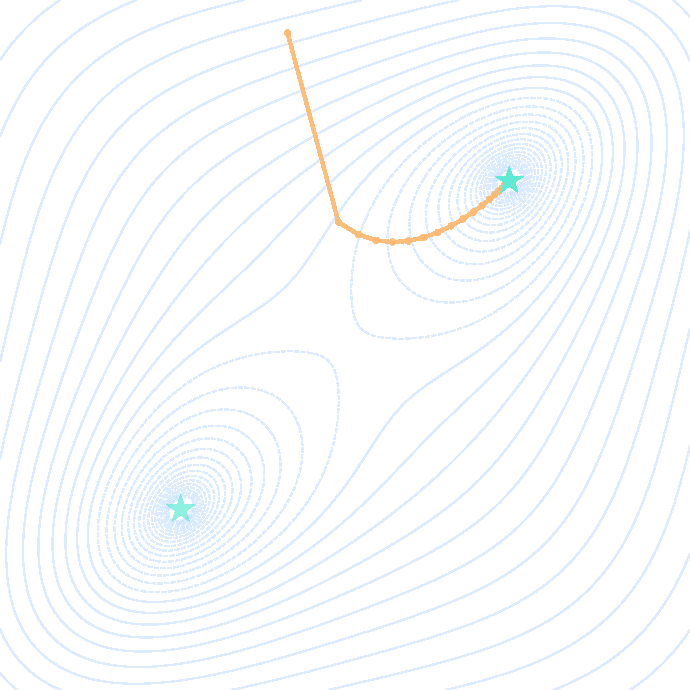
\includegraphics[height=1.05\paperheight]{fig_title_bg}};
    \fill[mNavy, path fading=east] (current page.south west) rectangle ([xshift=-3.4cm]current page.north east);
    \node[anchor=north west, text width=0.62\paperwidth, align=left, inner sep=0pt]
      at ([xshift=1.0cm, yshift=-1.55cm]current page.north west) {%
        {\color{mOrangeLt}\scriptsize\bfseries CSE 401 \,\textperiodcentered\, NUMERICAL ANALYSIS, SIMULATION AND MODELING \,\textperiodcentered\, TOPIC 3}\\[10pt]
        {\color{white}\fontsize{28}{30}\selectfont\bfseries \inserttitle}\\[8pt]
        {\color{mSky}\normalsize \insertsubtitle}\\[12pt]
        {\color{mOrangeLt}\rule{2.2cm}{2pt}}\\[14pt]
        {\color{white}\large\bfseries Nawriz Ahmed Turjo}\\[3pt]
        {\color{mSky}\small Roll 2105032 \quad\textperiodcentered\quad \insertdate}};
  \end{tikzpicture}}

% =====================================================================
%  Section dividers: big section number, title, and a "you are here"
%  strip over the 12 stops of the roadmap.
% =====================================================================
\newcommand{\gm@stoplabel}[1]{\ifcase#1 \or The problem\or The gradient\or Derivation\or Step size%
  \or Convergence\or Conditioning\or Failure modes\or Adaptive steps\or Acceleration%
  \or SGD and modern\or Applications\or Part B\fi}
\newcommand{\gm@stop}{\ifcase\value{section} 0\or 1\or 2\or 3\or 3\or 4\or 5\or 5\or 6\or 7\or 8\or 9%
  \or 10\or 10\or 99\or 12\else -1\fi}
\newcommand{\gm@secnum}{\ifcase\value{section}\or 01\or 02\or 03\or 04\or 05\or 06\or 07\or 08\or 09%
  \or 10\or 11\or 12\or 13\or 14\or B\else R\fi}
\newcommand{\gm@stopstrip}{%
  \edef\gm@cur{\gm@stop}%
  \ifnum\gm@cur>-1
  \begin{tikzpicture}[x=0.78cm]
    \draw[mNavy!25, line width=1.2pt] (1,0) -- (12,0);
    \foreach \i in {1,...,12}{%
      \ifnum\gm@cur=99
        \ifnum\i<11 \fill[mNavy] (\i,0) circle (2.6pt);
        \else \fill[mPaper] (\i,0) circle (2.6pt); \draw[mNavy!45, line width=0.8pt] (\i,0) circle (2.6pt); \fi
      \else
        \ifnum\i<\gm@cur \fill[mNavy] (\i,0) circle (2.6pt);
        \else\ifnum\i=\gm@cur
          \fill[mOrange] (\i,0) circle (4.6pt); \fill[mPaper] (\i,0) circle (1.6pt);
          \node[below=5pt, font=\scriptsize\bfseries, mOrange] at (\i,0) {\gm@stoplabel{\i}};
        \else
          \fill[mPaper] (\i,0) circle (2.6pt); \draw[mNavy!45, line width=0.8pt] (\i,0) circle (2.6pt);
        \fi\fi
      \fi}
    \ifnum\gm@cur=99 \node[below=5pt, font=\scriptsize\bfseries, mOrange] at (5.5,0) {Part A recap}; \fi
    \node[left=4pt, font=\tiny, mGrey] at (1,0) {start};
    \node[right=4pt, font=\tiny, mGrey] at (12,0) {Part B};
  \end{tikzpicture}%
  \fi}
\setbeamertemplate{section page}{%
  \begin{minipage}{0.86\textwidth}
    \raggedright
    {\fontsize{46}{46}\selectfont\bfseries\color{mOrange}\gm@secnum}\\[4pt]
    {\usebeamerfont{section title}\usebeamercolor[fg]{section title}\insertsectionhead}\\[2pt]
    {\color{mOrange}\rule{1.6cm}{2pt}}\\[18pt]
    \gm@stopstrip
  \end{minipage}}
\makeatother

% =====================================================================
%  Boxes: a coloured bar on the left instead of a heavy frame.
% =====================================================================
\tcbset{
  gmbase/.style={enhanced, breakable=false, frame hidden, sharp corners,
                 borderline west={2.6pt}{0pt}{#1},
                 colback=#1!6!mPaper, colbacktitle=#1!6!mPaper, coltitle=#1,
                 titlerule=0pt, toptitle=3pt, bottomtitle=-1pt,
                 left=8pt, right=6pt, top=3pt, bottom=4pt,
                 fonttitle=\bfseries\small, fontupper=\small,
                 before skip=5pt, after skip=5pt}
}
\newtcolorbox{probbox}[1][]{gmbase=mOrange, title={#1}}
\newtcolorbox{thmbox}[1][]{gmbase=mNavy, title={#1}}
\newtcolorbox{keybox}[1][]{gmbase=mTeal, title={#1}}
\newtcolorbox{warnbox}[1][]{gmbase=mRed, title={#1}}

% boxed answers: rounded teal outline, same treatment everywhere
\newtcbox{\anstcb}{on line, enhanced, colback=mTeal!8!mPaper, colframe=mTeal, boxrule=0.7pt,
  arc=2.5pt, left=2.5pt, right=2.5pt, top=1pt, bottom=1pt, boxsep=0.6pt}
\newcommand{\ans}[1]{\text{\anstcb{$\displaystyle #1$}}}

% =====================================================================
%  Part B: navy strip with the problem id on the left edge, and step dots
%  in the solution titles.
% =====================================================================
\gdef\gmprob{}
\newcommand{\setprob}[1]{\gdef\gmprob{#1}}
\setbeamertemplate{background}{%
  \ifx\gmprob\empty\else
  \begin{tikzpicture}
    \useasboundingbox (0,0) rectangle (\paperwidth,\paperheight);
    \fill[mNavy] (0,0.8cm) rectangle (0.36cm,\paperheight);   % stops above the footer
    \node[rotate=90, text=white, font=\scriptsize\bfseries, inner sep=0pt] at (0.18cm,0.55\paperheight)
      {PROBLEM \gmprob};
  \end{tikzpicture}%
  \fi}
\makeatletter
\def\gm@dots#1#2#3{%
  \ifnum#1>#3\relax\else
    \ifnum#1>#2\relax{\color{mNavy!25}\textbullet}\else{\color{mOrange}\textbullet}\fi
    \expandafter\gm@dots\expandafter{\the\numexpr#1+1\relax}{#2}{#3}%
  \fi}
\newcommand{\stepdots}[2]{{\normalsize\gm@dots{1}{#1}{#2}}}
\makeatother

% \probtitle{M1}{Stationary points}   -> "Problem M1 · Stationary points"
\newcommand{\probtitle}[2]{Problem #1 \textperiodcentered\ #2}
\newcommand{\soltitle}[3]{Problem #1 \textperiodcentered\ Solution #2/#3 \;\stepdots{#2}{#3}}

% =====================================================================
%  Maths macros
% =====================================================================
\newcommand{\R}{\mathbb{R}}
\newcommand{\E}{\mathbb{E}}
\newcommand{\x}{\mathbf{x}}
\newcommand{\y}{\mathbf{y}}
\newcommand{\e}{\mathbf{e}}
\newcommand{\g}{\mathbf{g}}
\newcommand{\vb}{\mathbf{b}}
\newcommand{\vd}{\mathbf{d}}
\newcommand{\vu}{\mathbf{u}}
\renewcommand{\vv}{\mathbf{v}}   % newtxsf defines a vector accent with this name
\newcommand{\vf}{\mathbf{f}}
\newcommand{\bA}{\mathbf{A}}
\newcommand{\bH}{\mathbf{H}}
\newcommand{\bI}{\mathbf{I}}
\newcommand{\bK}{\mathbf{K}}
\newcommand{\bP}{\mathbf{P}}
\newcommand{\T}{^{\mathsf T}}
\newcommand{\grad}{\nabla f}
\newcommand{\norm}[1]{\left\lVert #1 \right\rVert}
\newcommand{\abs}[1]{\left\lvert #1 \right\rvert}
\newcommand{\ip}[2]{\left\langle #1, #2 \right\rangle}
\newcommand{\lmin}{\lambda_{\min}}
\newcommand{\lmax}{\lambda_{\max}}
\providecommand{\SSR}{\mathrm{SSR}}
\providecommand{\w}{\mathbf{w}}
\DeclareMathOperator*{\argmin}{arg\,min}
\DeclareMathOperator*{\argmax}{arg\,max}
\DeclareMathOperator{\diag}{diag}

% =====================================================================
%  Statement slides (big idea, dark navy, large type)
% =====================================================================
% \statement{KICKER}{Big sentence}{small follow-up}
\newcommand{\statement}[3]{%
  \begin{frame}[standout]
    \begin{minipage}{0.84\textwidth}\centering
      {\color{mOrangeLt}\scriptsize\bfseries #1\par}\vspace{10pt}
      {\LARGE\bfseries\color{white} #2\par}\vspace{12pt}
      {\color{mOrangeLt}\rule{1.6cm}{1.6pt}\par}\vspace{10pt}
      {\color{mSky}\normalsize\mdseries #3\par}
    \end{minipage}
  \end{frame}}

% =====================================================================
%  Listings style
% =====================================================================
\lstdefinestyle{py}{
  language=Python, basicstyle=\ttfamily\scriptsize,
  keywordstyle=\color{mBlue}\bfseries, commentstyle=\color{mGrey}\itshape,
  stringstyle=\color{mTeal}, showstringspaces=false,
  frame=leftline, framerule=2.6pt, rulecolor=\color{mNavy}, backgroundcolor=\color{mLight},
  xleftmargin=6pt, xrightmargin=2pt, framesep=5pt, columns=fullflexible, keepspaces=true}

% tighter lists and display maths (Fira Sans is taller than the default font)
\setlength{\leftmargini}{1.2em}
\usepackage{etoolbox}
\makeatletter
\newcommand{\gm@tightdisplay}{%
  \setlength{\abovedisplayskip}{5pt plus 2pt minus 2pt}%
  \setlength{\belowdisplayskip}{5pt plus 2pt minus 2pt}%
  \setlength{\abovedisplayshortskip}{2pt plus 2pt}%
  \setlength{\belowdisplayshortskip}{4pt plus 2pt minus 2pt}}
\appto\normalsize{\gm@tightdisplay}
\appto\small{\gm@tightdisplay}
\appto\footnotesize{\gm@tightdisplay}
\makeatother
\setbeamertemplate{itemize/enumerate body begin}{\setlength{\itemsep}{1pt}}
\setbeamertemplate{itemize/enumerate subbody begin}{\setlength{\itemsep}{0pt}}

% numbered bibliography labels (match the [n] citations) instead of icons
\setbeamertemplate{bibliography item}{\insertbiblabel}
% run each entry on as one paragraph (beamer's defaults insert \par between blocks)
\setbeamertemplate{bibliography entry title}{}
\setbeamertemplate{bibliography entry location}{}
\setbeamertemplate{bibliography entry note}{}


\title{Gradient Methods}
\subtitle{From steepest descent to acceleration: theory, stability and practice}
\author{Nawriz Ahmed Turjo \quad|\quad Roll: 2105032}
\institute{CSE 401: Numerical Analysis, Simulation and Modeling \quad|\quad Assignment Topic 3}
\date{October 2026}

\begin{document}

% ---------------- Front matter ---------------------------------------
\maketitle

\begin{frame}{Assigned topic}
  \centering
  \vspace{6pt}
  {\Large\textbf{Topic 3: Gradient Methods}}

  \vspace{4pt}
  {\small One idea, $\x\gets\x-\alpha\nabla f(\x)$, and everything it takes to make it work.}

  \vspace{12pt}
  \begin{columns}[T]
    \begin{column}{0.46\textwidth}
      \begin{keybox}[Part A: the ideas]
        \small Where the method comes from and why it converges, how big a step can be, why it slows down,
        how it fails, and how momentum, adaptive steps and SGD fix it.
      \end{keybox}
    \end{column}
    \begin{column}{0.46\textwidth}
      \begin{probbox}[Part B: the problems]
        \small Five mathematical and five real-life problems, each followed straight away by a complete
        step-by-step solution.
      \end{probbox}
    \end{column}
  \end{columns}
\end{frame}

\begin{frame}{Where we are going}
  \centering
  \vspace{6pt}
  % Roadmap of the teaching story: three phases, numbered stops
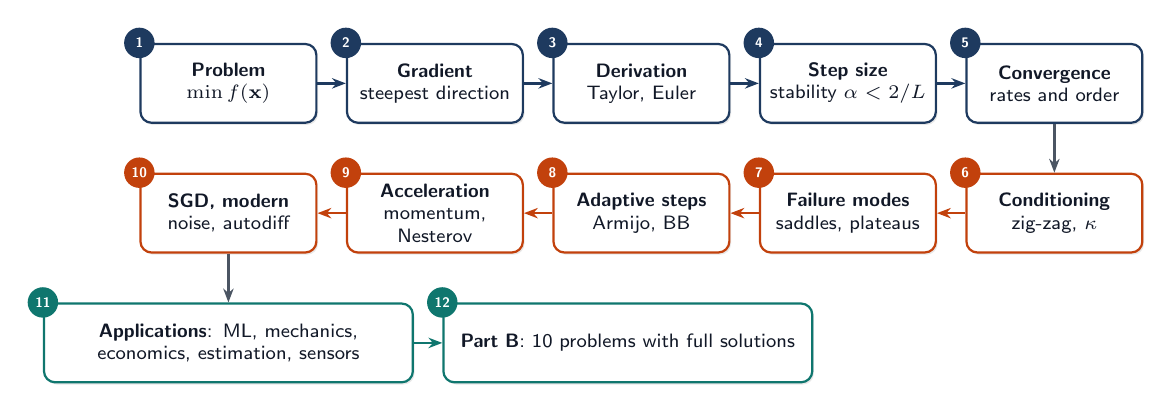
\begin{tikzpicture}[
  node distance=0.34cm and 0.36cm,
  stop/.style={draw=#1, line width=0.8pt, rounded corners=4pt, fill=white,
               drop shadow={opacity=0.18, shadow xshift=0.6pt, shadow yshift=-0.8pt},
               minimum height=1.0cm, text width=2.0cm, align=center, font=\scriptsize\color{mInk}},
  badge/.style={circle, fill=#1, text=white, font=\tiny\bfseries, inner sep=1.3pt, minimum size=11pt},
  arr/.style={-{Stealth[length=5pt]}, line width=0.9pt, #1},
  arr/.default=mGrey]
  % row 1: foundations (teal)
  \node[stop=mDarkTeal] (p) {\textbf{Problem}\\ $\min f(\x)$};
  \node[stop=mDarkTeal, right=of p] (g) {\textbf{Gradient}\\ steepest direction};
  \node[stop=mDarkTeal, right=of g] (d) {\textbf{Derivation}\\ Taylor, Euler};
  \node[stop=mDarkTeal, right=of d] (s) {\textbf{Step size}\\ stability $\alpha<2/L$};
  \node[stop=mDarkTeal, right=of s] (c) {\textbf{Convergence}\\ rates and order};
  % row 2: when it struggles and how to fix it (orange), right to left
  \node[stop=mOrange, below=0.62cm of c] (k) {\textbf{Conditioning}\\ zig-zag, $\kappa$};
  \node[stop=mOrange, left=of k] (f) {\textbf{Failure modes}\\ saddles, plateaus};
  \node[stop=mOrange, left=of f] (a) {\textbf{Adaptive steps}\\ Armijo, BB};
  \node[stop=mOrange, left=of a] (m) {\textbf{Acceleration}\\ momentum, Nesterov};
  \node[stop=mOrange, left=of m] (sg) {\textbf{SGD, modern}\\ noise, autodiff};
  % row 3: practice (green)
  \node[stop=mGreen, below=0.62cm of sg, text width=4.45cm] (ap) {\textbf{Applications}: ML, mechanics, economics, estimation, sensors};
  \node[stop=mGreen, right=of ap, text width=4.45cm] (pr) {\textbf{Part B}: 10 problems with full solutions};
  % arrows
  \draw[arr=mDarkTeal] (p) -- (g);  \draw[arr=mDarkTeal] (g) -- (d);
  \draw[arr=mDarkTeal] (d) -- (s);  \draw[arr=mDarkTeal] (s) -- (c);
  \draw[arr] (c.south) -- (k.north);
  \draw[arr=mOrange] (k) -- (f);  \draw[arr=mOrange] (f) -- (a);
  \draw[arr=mOrange] (a) -- (m);  \draw[arr=mOrange] (m) -- (sg);
  \draw[arr] (sg.south) -- (sg.south |- ap.north);
  \draw[arr=mGreen] (ap) -- (pr);
  % badges
  \foreach \n/\lab in {p/1, g/2, d/3, s/4, c/5}
    \node[badge=mDarkTeal] at (\n.north west) {\lab};
  \foreach \n/\lab in {k/6, f/7, a/8, m/9, sg/10}
    \node[badge=mOrange] at (\n.north west) {\lab};
  \node[badge=mGreen] at (ap.north west) {11};
  \node[badge=mGreen] at (pr.north west) {12};
\end{tikzpicture}


  \vspace{8pt}
  \footnotesize
  \textcolor{mDarkTeal}{\textbf{1--5}} how it works \qquad
  \textcolor{mOrange}{\textbf{6--10}} why it struggles, and the fixes \qquad
  \textcolor{mGreen}{\textbf{11--12}} putting it to use
\end{frame}

% ---------------- Part A: Concept presentation & theory -------------
\statement{PART A}{The ideas}{Where gradient descent comes from, why it works, and why it sometimes does not.}

% =====================================================================
%  1. Motivation and the optimization problem
% =====================================================================
\section{The optimization problem}

\begin{frame}{One question behind many problems}
  Train a model, settle a structure, plan production, fit data. Each asks: \alert{which input makes one number smallest?}

  \centering\small
  \begin{tabular}{@{}l l l@{}}
    \toprule
    Field & Unknown $\x$ & Objective $f(\x)$ to minimise \\
    \midrule
    Machine learning & model weights & training loss \\
    Structural mechanics & nodal displacements & potential energy \\
    Economics & production levels & $-$profit \\
    Parameter estimation & physical constants & sum of squared residuals \\
    Signal processing & filter or estimate & mean-squared error \\
    \bottomrule
  \end{tabular}

  \raggedright
  \begin{keybox}[The common form]
    \centering $\displaystyle \min_{\x\in\R^n} f(\x), \qquad f:\R^n\to\R \text{ differentiable}\quad\text{(maximise $P$ = minimise $-P$).}$
  \end{keybox}
\end{frame}

\begin{frame}{A first example: fitting a line to data}
  \begin{columns}[T]
    \begin{column}{0.5\textwidth}
      \small
      Predict height from weight with a straight line, $\hat y = b + m x$
      (intercept $b$, slope $m$).
      How good is a line? Add up the squared \alert{residuals} $r_i = y_i - (b + m x_i)$:
      \[
        \SSR(b, m) = \sum_{i=1}^{n}\bigl(y_i - b - m x_i\bigr)^2 .
      \]
      This is the \textbf{loss function}. The best line is the one with the smallest SSR.
      \begin{keybox}[Other uses]
        \footnotesize Linear and logistic regression, t-SNE: each one is ``pick the parameters that make a loss smallest''.
      \end{keybox}
    \end{column}
    \begin{column}{0.48\textwidth}
      \centering
      \only<1>{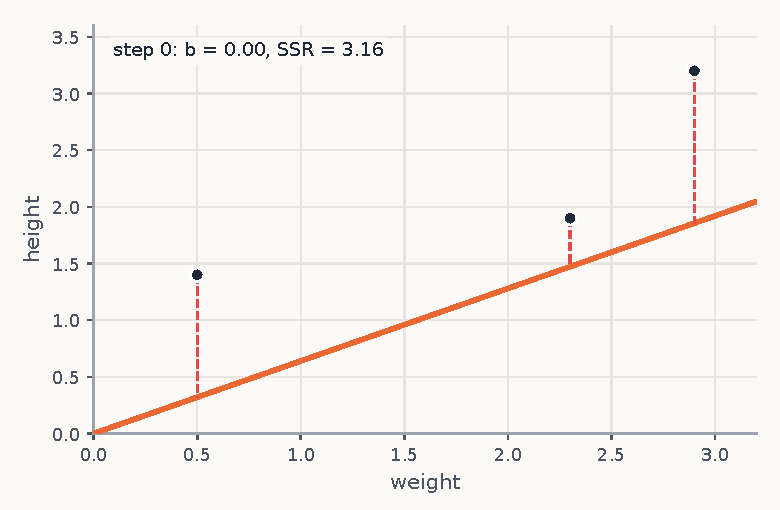
\includegraphics[width=\linewidth,height=0.55\textheight,keepaspectratio]{fig_line_frame_0}}%
      \only<2>{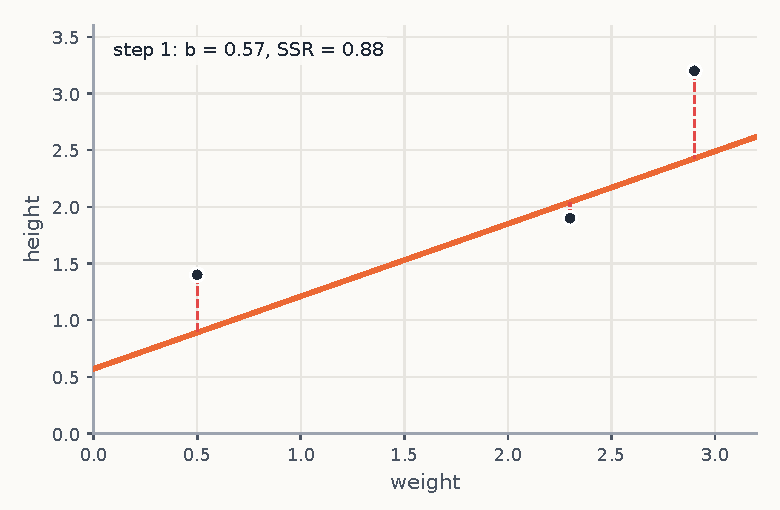
\includegraphics[width=\linewidth,height=0.55\textheight,keepaspectratio]{fig_line_frame_1}}%
      \only<3>{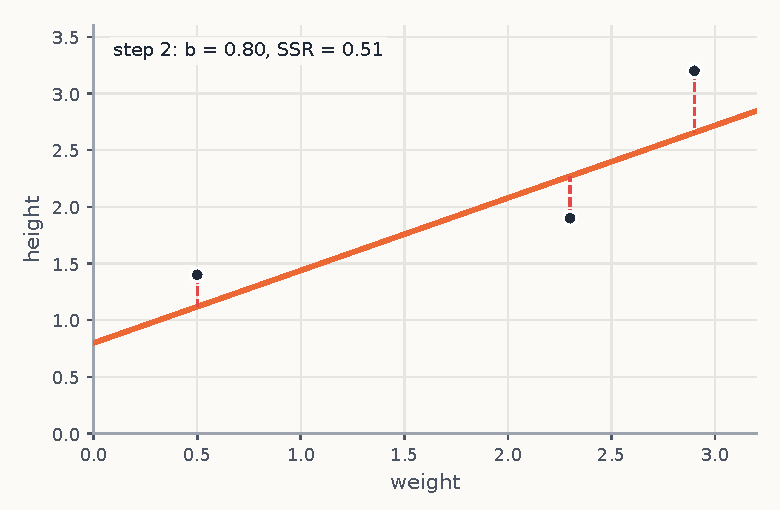
\includegraphics[width=\linewidth,height=0.55\textheight,keepaspectratio]{fig_line_frame_2}}%
      \only<4>{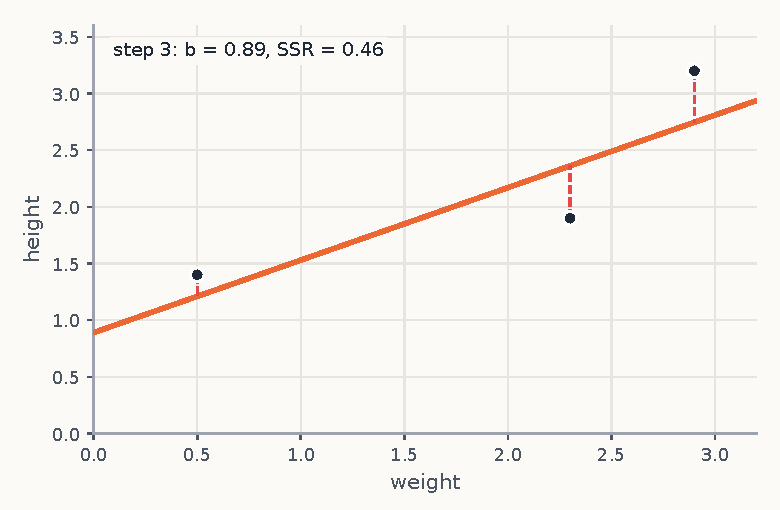
\includegraphics[width=\linewidth,height=0.55\textheight,keepaspectratio]{fig_line_frame_3}}%
      \only<5>{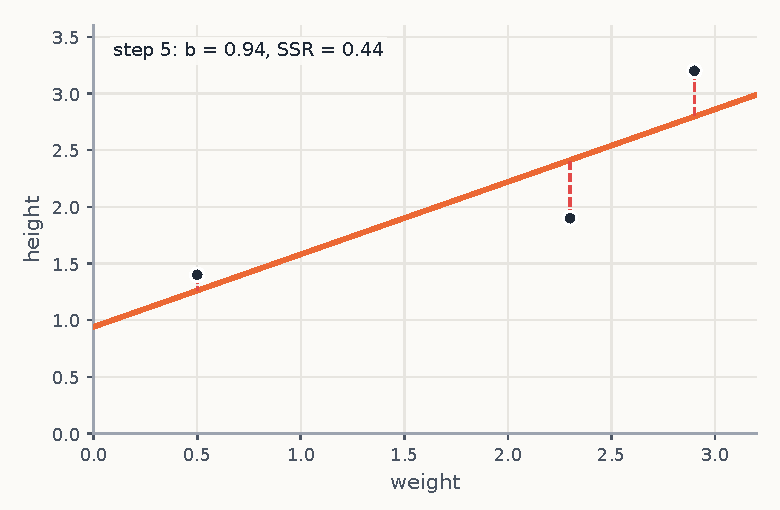
\includegraphics[width=\linewidth,height=0.55\textheight,keepaspectratio]{fig_line_frame_4}}%
      \only<6>{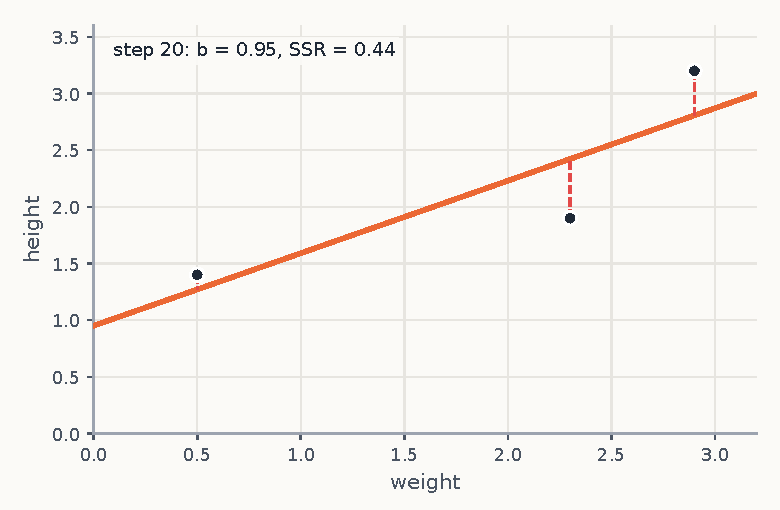
\includegraphics[width=\linewidth,height=0.55\textheight,keepaspectratio]{fig_line_frame_5}}%

      \footnotesize Data: weights $0.5, 2.3, 2.9$, heights $1.4, 1.9, 3.2$. Each click shows smaller residuals.
    \end{column}
  \end{columns}
\end{frame}

\begin{frame}{What counts as a solution?}
  \small
  $\x^\star$ is a \textbf{global minimiser} if $f(\x^\star)\le f(\x)$ for every $\x$, and a \textbf{local minimiser}
  if that only holds near $\x^\star$.
  \begin{thmbox}[First-order necessary condition]
    If $\x^\star$ is a local minimiser and $f$ is differentiable, then $\nabla f(\x^\star) = \mathbf 0$.
  \end{thmbox}
  \textbf{Proof.} Suppose $\g = \nabla f(\x^\star)\ne\mathbf 0$. Then
  $f(\x^\star - t\g) = f(\x^\star) - t\norm{\g}^2 + o(t) < f(\x^\star)$ for small $t>0$, so $\x^\star$ was not a minimiser. $\blacksquare$

  \vspace{4pt}
  \begin{itemize}\small
    \item Second order: $\nabla^2 f(\x^\star)\succeq 0$ is necessary, and $\nabla f = \mathbf 0$ with $\nabla^2 f\succ0$ is sufficient.
    \item A zero gradient does not guarantee a minimum. $x^4+y^4-4xy$ has a \alert{saddle} at the origin (Problem M1).
  \end{itemize}
\end{frame}

\begin{frame}{Why not just solve $\nabla f = \mathbf 0$?}
  \begin{itemize}\small
    \item $\nabla f(\x) = \mathbf 0$ is a system of $n$ \emph{nonlinear} equations, and closed-form solutions are rare.
    \item Second-order methods use the Hessian, which costs $n^2$ memory and $O(n^3)$ work per linear solve.
          They are a separate topic and appear here only for contrast.
    \item \textbf{First-order methods} need only $\nabla f$: $O(n)$ memory and one gradient per iteration.
          That is cheap enough for $n\sim10^9$, the size of modern neural networks.
  \end{itemize}

  \vspace{4pt}
  \begin{columns}[T]
    \begin{column}{0.58\textwidth}
      \begin{keybox}[A little history]
        \small Cauchy proposed steepest descent in 1847 to solve systems of simultaneous equations,
        by driving a nonnegative function down to zero~\cite{cauchy1847}. More than 175 years later,
        variants of the same idea train today's largest models~\cite{bottou2018}.
      \end{keybox}
    \end{column}
    \begin{column}{0.4\textwidth}
      \small
      \textbf{In this module we}
      \begin{itemize}\footnotesize
        \item derive gradient descent and prove how fast it converges,
        \item find out \emph{when} and \emph{why} it slows down,
        \item fix it with adaptive steps, momentum and SGD.
      \end{itemize}
    \end{column}
  \end{columns}
\end{frame}

% =====================================================================
%  2. Gradient and directional derivative
% =====================================================================
\section{The gradient: which way is downhill?}

\begin{frame}{Gradient and directional derivative}
  \begin{itemize}\small
    \item The gradient collects all partial derivatives: $\nabla f(\x) = \bigl(\tfrac{\partial f}{\partial x_1},\dots,\tfrac{\partial f}{\partial x_n}\bigr)\T$.
    \item The directional derivative along $\vd$ tells you how fast $f$ changes if you move that way
          (chain rule on $t\mapsto f(\x+t\vd)$):
  \end{itemize}
  \[
    D_{\vd} f(\x) = \lim_{t\to0}\frac{f(\x + t\vd) - f(\x)}{t} = \nabla f(\x)\T\vd .
  \]
  \begin{itemize}\small
    \item First-order Taylor expansion: $f(\x + t\vd) = f(\x) + t\,\nabla f(\x)\T\vd + o(t)$.
    \item So if $\nabla f(\x)\T\vd < 0$, a small step along $\vd$ lowers $f$. We call $\vd$ a \alert{descent direction}.
  \end{itemize}
  \begin{keybox}[The question that starts everything]
    Of all the unit directions you could step in, which one lowers $f$ the \emph{fastest}?
  \end{keybox}
\end{frame}

\begin{frame}{Theorem: $-\nabla f$ is the steepest way down}
  \begin{columns}[T]
    \begin{column}{0.55\textwidth}
      \begin{thmbox}[Theorem (steepest descent)]
        If $\nabla f(\x)\neq\mathbf 0$, then
        \[
          \min_{\norm{\vd}=1}\nabla f(\x)\T\vd = -\norm{\nabla f(\x)},
        \]
        and the only minimiser is $\vd^\star = -\nabla f(\x)/\norm{\nabla f(\x)}$.
      \end{thmbox}
      \small\textbf{Proof.}
      \pause
      By Cauchy--Schwarz, $|\nabla f\T\vd| \le \norm{\nabla f}\norm{\vd} = \norm{\nabla f}$, so
      $\nabla f\T\vd \ge -\norm{\nabla f}$.
      \pause
      Cauchy--Schwarz is an equality only when $\vd$ is parallel to $\nabla f$. Taking the minus sign,
      $\vd = -\nabla f/\norm{\nabla f}$ reaches the bound. $\blacksquare$
    \end{column}
    \begin{column}{0.43\textwidth}
      \centering
      % Steepest-descent geometry: the half-plane of descent directions, the unit
% circle of candidate directions d, the gradient and the angle theta.
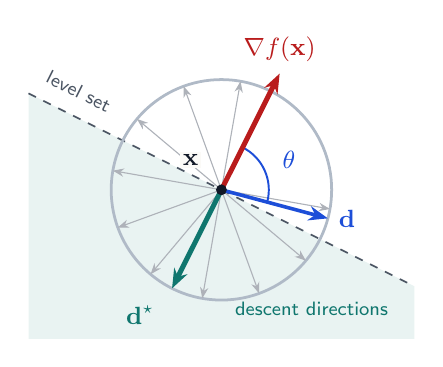
\begin{tikzpicture}[scale=1.4, >={Stealth[length=7pt]}]
  % descent half-plane  {d : grad^T d < 0}  (gradient direction (0.447, 0.894))
  \begin{scope}
    \clip (-1.75,-1.35) rectangle (1.75,1.35);
    \fill[mGreen!9] (-2,1) -- (2,-1) -- (2,-3) -- (-2,-3) -- cycle;
  \end{scope}
  \draw[mGrey, dashed, line width=0.6pt] (-1.75,0.875) -- (1.75,-0.875);
  \node[font=\scriptsize, mGreen, anchor=south east] at (1.60,-1.23) {descent directions};
  \node[font=\scriptsize, mGrey, rotate=-26.6, anchor=south west] at (-1.72,0.94) {level set};
  % unit circle
  \draw[mDarkTeal!35, line width=1pt] (0,0) circle (1);
  % candidate directions (faint)
  \foreach \t in {200,230,260,290,320,350,80,110,140,170}
    \draw[mGrey!45, -{Stealth[length=4pt]}] (0,0) -- (\t:1);
  % a generic direction d and the angle
  \draw[->, line width=1.3pt, mBlue] (0,0) -- (-15:1) node[right, font=\small] {$\vd$};
  \draw[mBlue, line width=0.7pt] (63.4:0.43) arc[start angle=63.4, end angle=-15, radius=0.43];
  \node[mBlue, font=\small] at (24:0.67) {$\theta$};
  % gradient and steepest descent
  \draw[->, line width=1.8pt, mRed] (0,0) -- (63.4:1.18) node[above, font=\small] {$\nabla f(\x)$};
  \draw[->, line width=1.8pt, mGreen] (0,0) -- (243.4:1) node[below left=3pt, font=\small] {$\vd^\star$};
  \fill[mInk] (0,0) circle (1.4pt);
  \node[font=\small, mInk, fill=mPaper, inner sep=1pt] at (-0.28,0.27) {$\x$};
\end{tikzpicture}


      \footnotesize $D_{\vd}f = \norm{\nabla f}\cos\theta$, which is smallest at $\theta = \pi$.
      Every arrow in the green half-plane goes downhill; $\vd^\star$ goes down fastest.
    \end{column}
  \end{columns}
\end{frame}

\begin{frame}{The gradient is perpendicular to the contours}
  \begin{columns}[T]
    \begin{column}{0.47\textwidth}
      \small
      Take any smooth curve $\gamma(t)$ that stays on the level set $\{f = c\}$, with $\gamma(0) = \x$. Then
      \[
        f(\gamma(t)) = c \;\Rightarrow\; \nabla f(\x)\T\gamma'(0) = 0 .
      \]
      So $\nabla f(\x)$ is perpendicular to every direction along the contour.

      \vspace{4pt}
      \begin{itemize}\footnotesize
        \item The arrows show $-\nabla f$ (normalised) for $f = x^4+y^4-4xy$.
        \item Look at how they cross every contour at a right angle, run away from the saddle along $(1,1)$,
              and pour into the two minima.
      \end{itemize}
    \end{column}
    \begin{column}{0.51\textwidth}
      \centering
      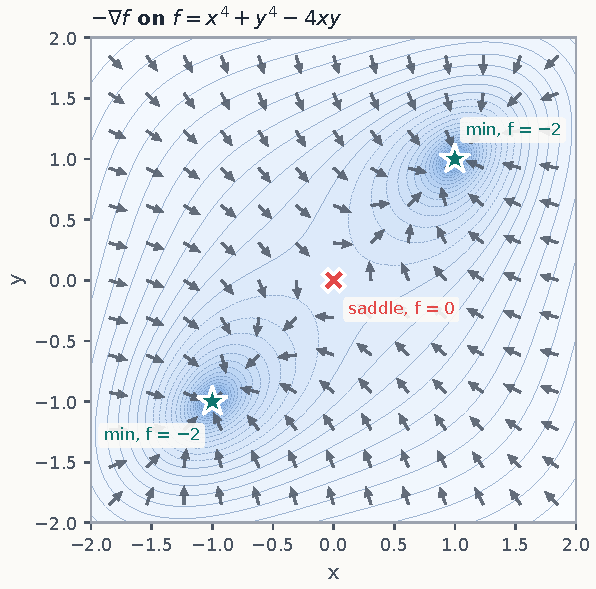
\includegraphics[width=0.92\linewidth]{fig_landscape_contour}
    \end{column}
  \end{columns}
\end{frame}

\begin{frame}{``Steepest'' depends on how you measure length}
  Swap the Euclidean norm for $\norm{\vd}_{\bP} = \sqrt{\vd\T\bP\vd}$ with $\bP\succ0$, and the answer changes:
  \[
    \min_{\vd\T\bP\vd\le1}\nabla f\T\vd
    \quad\Longrightarrow\quad
    \vd^\star \propto -\bP^{-1}\nabla f(\x).
  \]
  \small\textbf{Proof.} Substitute $\vd = \bP^{-1/2}\mathbf z$ with $\norm{\mathbf z}\le1$. The objective becomes
  $(\bP^{-1/2}\nabla f)\T\mathbf z$, so the previous theorem gives $\mathbf z^\star\propto-\bP^{-1/2}\nabla f$ and therefore
  $\vd^\star\propto-\bP^{-1}\nabla f$. $\blacksquare$

  \vspace{4pt}
  \begin{center}
  \begin{tabular}{@{}l l@{}}
    \toprule
    Choice of $\bP$ & What you get \\
    \midrule
    $\bI$ & plain gradient descent \\
    a diagonal scaling & feature standardisation, Adam-type methods (Section~13) \\
    $\nabla^2 f(\x)$ & the Newton direction (a different topic, mentioned only) \\
    \bottomrule
  \end{tabular}
  \end{center}
  \footnotesize\textcolor{mGrey}{So there is no single ``steepest'' direction. It depends on the geometry you pick~\cite{boyd2004},
  and choosing that geometry well is what preconditioning does (Section~8).}
\end{frame}

% =====================================================================
%  3. Deriving gradient descent: Taylor, majorisation, gradient flow
% =====================================================================
\section{Three ways to arrive at gradient descent}

\begin{frame}{View 1: trust the linear model, but only nearby}
  The Taylor model at $\x_k$ is good close to $\x_k$ and gets worse as you move away. So minimise the model
  plus a penalty for going too far:
  \[
    \x_{k+1} = \argmin_{\x}\;\Bigl\{\underbrace{f(\x_k) + \nabla f(\x_k)\T(\x - \x_k)}_{\text{linear model}}
      + \underbrace{\tfrac{1}{2\alpha}\norm{\x - \x_k}^2}_{\text{stay close}}\Bigr\}.
  \]
  Set the gradient of the braces to zero:
  \[
    \nabla f(\x_k) + \tfrac1\alpha(\x - \x_k) = \mathbf 0
    \quad\Longrightarrow\quad
    \ans{\x_{k+1} = \x_k - \alpha\,\nabla f(\x_k)}
  \]
  \begin{itemize}\small
    \item $\alpha$ is the \alert{step size} (the ``learning rate'' in ML). A large $\alpha$ means we trust the linear model further out.
    \item Change the penalty and you get a different method. With $\tfrac12\norm{\cdot}_{\bP}^2$ you get preconditioned GD (Section~2).
  \end{itemize}
\end{frame}

\begin{frame}{View 2: minimise an upper bound}
  \begin{columns}[T]
    \begin{column}{0.47\textwidth}
      \small
      If $\nabla f$ is $L$-Lipschitz, the \emph{descent lemma} (Section~7, Problem M2) says that for every $\x$
      \[
        f(\x) \le f(\x_k) + \nabla f(\x_k)\T(\x-\x_k) + \tfrac L2\norm{\x-\x_k}^2 .
      \]
      \begin{itemize}\footnotesize
        \item That is View 1 with $\alpha = 1/L$, except now the model is an \alert{upper bound} touching $f$ at $\x_k$.
        \item Its minimiser is $\x_{k+1} = \x_k - \tfrac1L\nabla f(\x_k)$.
        \item $f(\x_{k+1}) \le$ bound at $\x_{k+1}$ $\le$ bound at $\x_k = f(\x_k)$, so $f$ \alert{has to go down}.
      \end{itemize}
      \footnotesize\textcolor{mGrey}{This trick is known as majorise and minimise (MM).}
    \end{column}
    \begin{column}{0.51\textwidth}
      \centering
      % 1-D descent lemma: f, tangent line, quadratic upper bound touching at x_k,
% the GD step as the minimiser of the upper bound, and the guaranteed drop.
% f(x) = 0.35 x^2 + 0.5 cos(2x) + 0.6  (f'' <= 0.7 + 2 = 2.7, so L = 2.7)
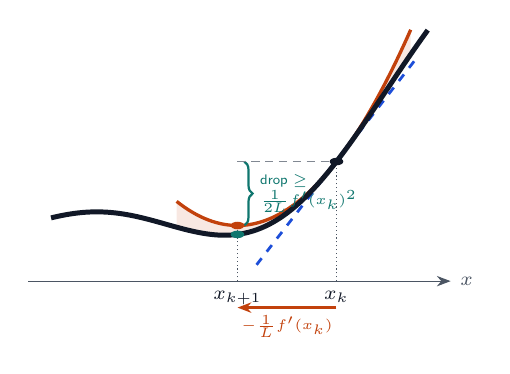
\begin{tikzpicture}[xscale=1.45, yscale=0.8, >={Stealth[length=5pt]},
  declare function={f(\x)=0.35*\x*\x + 0.5*cos(deg(2*\x)) + 0.6;
                    fp(\x)=0.7*\x - sin(deg(2*\x));
                    q(\x)=f(2.1) + fp(2.1)*(\x-2.1) + 0.5*2.7*(\x-2.1)*(\x-2.1);}]
  \def\xk{2.1}
  \def\Lc{2.7}
  \pgfmathsetmacro{\xn}{\xk - fp(\xk)/\Lc}
  \pgfmathsetmacro{\fk}{f(\xk)}
  \pgfmathsetmacro{\qn}{\fk - fp(\xk)*fp(\xk)/(2*\Lc)}
  \pgfmathsetmacro{\fn}{f(\xn)}
  % gap between the upper model and f
  \fill[mOrange!12, domain=0.7:2.75, samples=60]
    plot (\x, {q(\x)}) -- plot[domain=2.75:0.7, samples=60] (\x, {f(\x)}) -- cycle;
  % axes
  \draw[->, mGrey] (-0.6,0) -- (3.1,0) node[right, font=\scriptsize] {$x$};
  % models and f
  \draw[line width=1pt, mBlue, dashed, domain=1.4:2.8] plot (\x, {\fk + fp(\xk)*(\x-\xk)});
  \draw[line width=1.2pt, mOrange, domain=0.7:2.75, samples=60] plot (\x, {q(\x)});
  \draw[line width=1.8pt, mInk, domain=-0.4:2.9, samples=100] plot (\x, {f(\x)});
  % drop lines and points
  \draw[mGrey, densely dotted] (\xk,0) node[below, font=\scriptsize, mInk] {$x_k$} -- (\xk,\fk);
  \draw[mGrey, densely dotted] (\xn,0) node[below, font=\scriptsize, mInk] {$x_{k+1}$} -- (\xn,\qn);
  \draw[->, line width=1pt, mOrange] (\xk,-0.42) -- node[below=-1pt, font=\tiny] {$-\tfrac1L f'(x_k)$} (\xn,-0.42);
  % guaranteed decrease bracket
  \draw[decorate, decoration={brace, amplitude=3pt, mirror}, mGreen, line width=0.8pt]
    (\xn+0.06,\qn) -- (\xn+0.06,\fk) node[midway, right=2pt, font=\tiny, align=left] {drop $\ge$\\$\frac{1}{2L}f'(x_k)^2$};
  \draw[mGrey!70, densely dashed] (\xn,\fk) -- (\xk,\fk);
  \fill[mInk] (\xk,\fk) circle (1.7pt);
  \fill[mOrange] (\xn,\qn) circle (1.7pt);
  \fill[mGreen] (\xn,\fn) circle (1.7pt);
\end{tikzpicture}


      \scriptsize
      \textcolor{mInk}{\rule[2pt]{10pt}{1.8pt}} $f$ \quad
      \textcolor{mBlue}{\rule[2pt]{10pt}{1pt}} tangent \quad
      \textcolor{mOrange}{\rule[2pt]{10pt}{1.2pt}} upper model (curvature $L$)\\
      \textcolor{mOrange}{$\bullet$} minimum of the model, \quad \textcolor{mGreen}{$\bullet$} the true $f(x_{k+1})$, lower still.
    \end{column}
  \end{columns}
\end{frame}

\begin{frame}{View 3, the central idea: GD is forward Euler on the gradient flow}
  The \textbf{gradient flow} ODE $\;\dot\x(t) = -\nabla f(\x(t))$ always runs downhill:
  \[
    \frac{d}{dt}f(\x(t)) = \nabla f\T\dot\x = -\norm{\nabla f(\x(t))}^2 \le 0 .
  \]
  Now discretise it with \textbf{forward Euler}, step $h$: $\;\x_{k+1} = \x_k + h\,(-\nabla f(\x_k))$.
  That is \alert{gradient descent with $\alpha = h$}. Everything we know about Euler's method now applies.

  \vspace{4pt}
  \centering\small
  \begin{tabular}{@{}l l@{}}
    \toprule
    What we know from ODEs & What it means for optimisation \\
    \midrule
    Euler stability interval $|1 - h\lambda| < 1$ & the step limit $\alpha < 2/L$ (Section~5) \\
    stiffness (widely spread eigenvalues) & ill-conditioning and the zig-zag (Section~8) \\
    implicit (backward) Euler & the proximal-point method, stable for any step \\
    second-order ODE with friction & heavy-ball momentum (Section~11) \\
    $\ddot\x + \tfrac3t\dot\x + \nabla f = 0$ & Nesterov acceleration~\cite{su2016} \\
    \bottomrule
  \end{tabular}
\end{frame}

\statement{THE CENTRAL IDEA}{Gradient descent is forward Euler\\ on the gradient flow.}{So the step limit is a stability limit, and ill-conditioning is stiffness.}

\begin{frame}{The algorithm}
  \begin{columns}[T]
    \begin{column}{0.52\textwidth}
      \begin{thmbox}[Algorithm: gradient descent]
        \small
        \textbf{Input:} $\x_0$, step $\alpha>0$, tolerances $\varepsilon_{\text{rel}},\varepsilon_{\text{abs}}$, $k_{\max}$\\[2pt]
        \textbf{for} $k = 0,1,2,\dots,k_{\max}-1$:\\
        \quad $\g_k \gets \nabla f(\x_k)$\\
        \quad \textbf{if} $\norm{\g_k}\le\varepsilon_{\text{rel}}\norm{\g_0}+\varepsilon_{\text{abs}}$: \textbf{stop}\\
        \quad $\x_{k+1}\gets\x_k - \alpha\,\g_k$\\
        \textbf{return} $\x_k$
      \end{thmbox}
    \end{column}
    \begin{column}{0.46\textwidth}
      \small\textbf{When should it stop?}
      \begin{itemize}\footnotesize
        \item A small $\norm{\nabla f}$ is the natural test. For strongly convex $f$ it even bounds the error:
              $\norm{\x-\x^\star}\le\norm{\nabla f(\x)}/\mu$ (Section~6).
        \item Stopping only because $|f_{k+1}-f_k|$ is tiny is a trap. On a plateau $f$ hardly changes
              while $\x$ is still far from the answer (Problem A4).
        \item Always cap the iteration count and use a relative tolerance, because floating point limits
              how small the gradient can get (Section~9).
      \end{itemize}
    \end{column}
  \end{columns}
\end{frame}

\begin{frame}{One parameter by hand: the line fit, with numbers}
  \small
  Fix the slope at $m = 0.64$ and let GD find the intercept $b$, starting from $b_0 = 0$ with learning rate $\alpha = 0.1$.
  \[
    \frac{d\,\SSR}{db} = -2\sum_{i}\bigl(y_i - b - 0.64\,x_i\bigr),\quad
    \text{step} = \frac{d\,\SSR}{db}\times\alpha,\quad b_{\text{new}} = b_{\text{old}} - \text{step}.
  \]
  \centering\footnotesize
  \begin{tabular}{@{}c c c c c@{}}
    \toprule
    step $k$ & $b_k$ & slope $d\SSR/db$ & step size & $\SSR(b_{k+1})$ \\
    \midrule
    0 & $0$ & $-5.704$ & $-0.5704$ & $0.878$ \\
    1 & $0.5704$ & $-2.282$ & $-0.2282$ & $0.514$ \\
    2 & $0.7986$ & $-0.913$ & $-0.0913$ & $0.456$ \\
    3 & $0.8898$ & $-0.365$ & $-0.0365$ & $0.446$ \\
    \bottomrule
  \end{tabular}

  \raggedright
  \vspace{4pt}
  Each step is about $0.4\times$ the last (start $\SSR = 3.156$), and $b$ settles at \ans{b^\star = 0.951}.\par
  Steps shrink because the slope flattens near the minimum.
\end{frame}

\begin{frame}{Several parameters: the same recipe, once per parameter}
  \begin{columns}[T]
    \begin{column}{0.46\textwidth}
      \centering
      \scalebox{0.9}{% Gradient descent loop, steps (i)-(vi)
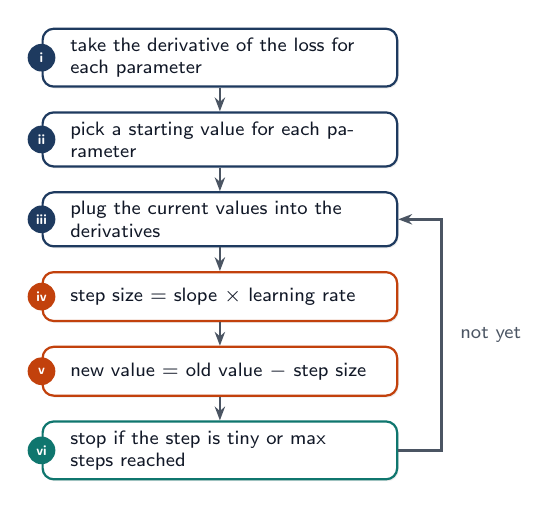
\begin{tikzpicture}[
  node distance=0.30cm,
  step/.style={draw=#1, line width=0.8pt, rounded corners=4pt, fill=white,
               drop shadow={opacity=0.15, shadow xshift=0.5pt, shadow yshift=-0.7pt},
               text width=3.8cm, minimum height=0.62cm, align=left, font=\scriptsize\color{mInk},
               inner xsep=10pt},
  step/.default=mNavy,
  badge/.style={circle, fill=#1, text=white, font=\tiny\bfseries, inner sep=1pt, minimum size=10pt},
  arr/.style={-{Stealth[length=5pt]}, line width=0.9pt, mGrey}]
  \node[step] (s1) {take the derivative of the loss for each parameter};
  \node[step, below=of s1] (s2) {pick a starting value for each parameter};
  \node[step, below=of s2] (s3) {plug the current values into the derivatives};
  \node[step=mOrange, below=of s3] (s4) {step size $=$ slope $\times$ learning rate};
  \node[step=mOrange, below=of s4] (s5) {new value $=$ old value $-$ step size};
  \node[step=mTeal, below=of s5] (s6) {stop if the step is tiny or max steps reached};
  \foreach \a/\b in {s1/s2, s2/s3, s3/s4, s4/s5, s5/s6} \draw[arr] (\a) -- (\b);
  \draw[arr] (s6.east) -- ++(0.55,0) |- node[pos=0.25, right=3pt, font=\scriptsize, mGrey] {not yet} (s3.east);
  \foreach \n/\lab/\c in {s1/i/mNavy, s2/ii/mNavy, s3/iii/mNavy, s4/iv/mOrange, s5/v/mOrange, s6/vi/mTeal}
    \node[badge=\c] at (\n.west) {\lab};
\end{tikzpicture}
}
    \end{column}
    \begin{column}{0.52\textwidth}
      \small
      For $\hat y = b + mx$ both parameters move:
      \begin{align*}
        \frac{\partial\SSR}{\partial b} &= -2\sum_i\bigl(y_i - b - m x_i\bigr),\\
        \frac{\partial\SSR}{\partial m} &= -2\sum_i x_i\bigl(y_i - b - m x_i\bigr).
      \end{align*}
      In general, for every $w_j$ at once:
      \[
        \ans{w_j \leftarrow w_j - \alpha\,\frac{\partial f}{\partial w_j}}
      \]
      \textbf{Stop} when the step size is near zero (say $<10^{-3}$) or after a maximum number of steps.
    \end{column}
  \end{columns}
\end{frame}

\begin{frame}[fragile]{The whole method in a dozen lines}
  \begin{columns}[T]
    \begin{column}{0.55\textwidth}
\begin{lstlisting}[style=py]
import numpy as np

def gradient_descent(grad, x0, alpha,
                     rtol=1e-8, maxit=10_000):
    x = np.asarray(x0, dtype=float).copy()
    g0 = np.linalg.norm(grad(x))
    for k in range(maxit):
        g = grad(x)
        if np.linalg.norm(g) <= rtol * g0:
            break
        x -= alpha * g       # O(n) update
    return x, k

# least squares: f(w) = ||Xw - y||^2 / (2m)
def ls_grad(w, X, y):
    return X.T @ (X @ w - y) / len(y)
\end{lstlisting}
    \end{column}
    \begin{column}{0.43\textwidth}
      \small\textbf{What one iteration costs}
      \begin{itemize}\footnotesize
        \item One gradient and an $O(n)$ vector update, with $O(n)$ memory.
        \item For least squares with $\mathbf X\in\R^{m\times n}$, that is two matrix--vector products, $O(mn)$.
              Nothing gets factorised.
        \item Written with array operations (BLAS, GPUs) instead of Python loops, the same code runs for
              $n = 2$ or for millions of variables.
        \item Total cost is (number of iterations) $\times$ (cost of $\nabla f$). The rest of the module is
              about that first factor.
      \end{itemize}
    \end{column}
  \end{columns}
\end{frame}

% =====================================================================
%  4. Geometric interpretation (overlay animation)
% =====================================================================
\section{Watching it move}

\begin{frame}{Gradient descent, one step at a time}
  \begin{columns}[T]
    \begin{column}{0.62\textwidth}
      \centering
      \only<1>{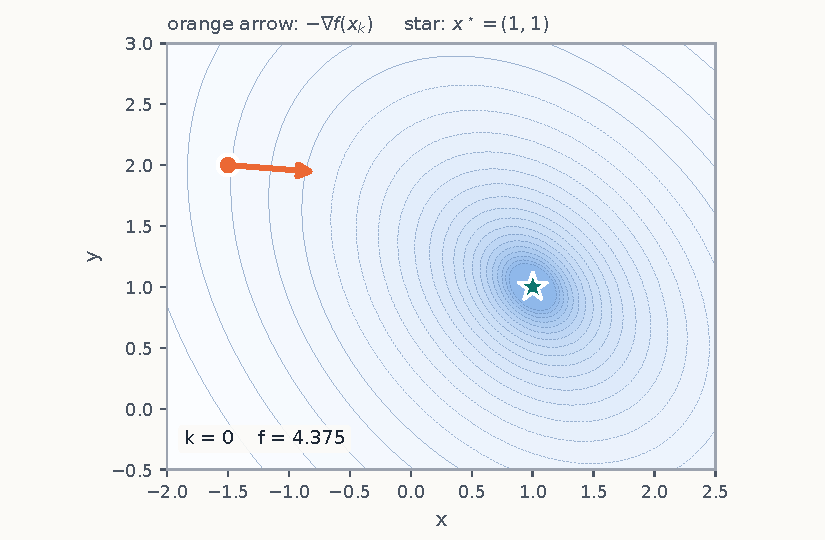
\includegraphics[height=0.70\textheight]{fig_gd_frame_0}}%
      \only<2>{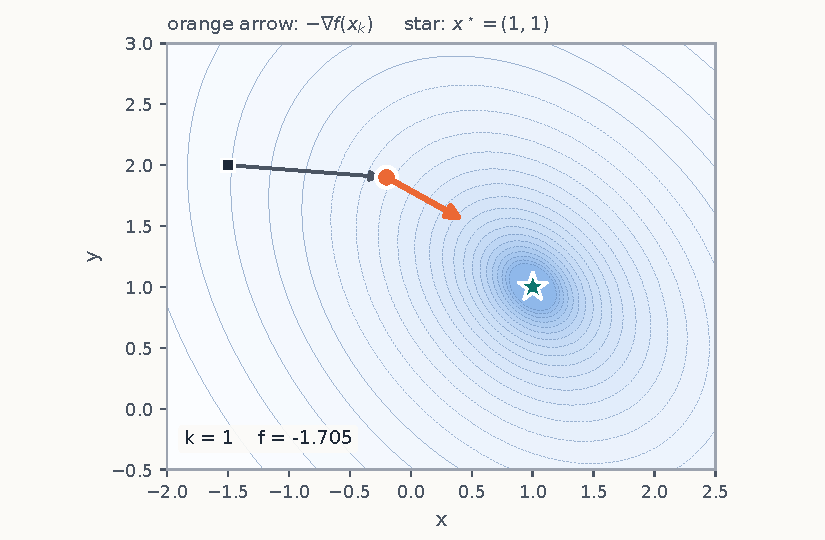
\includegraphics[height=0.70\textheight]{fig_gd_frame_1}}%
      \only<3>{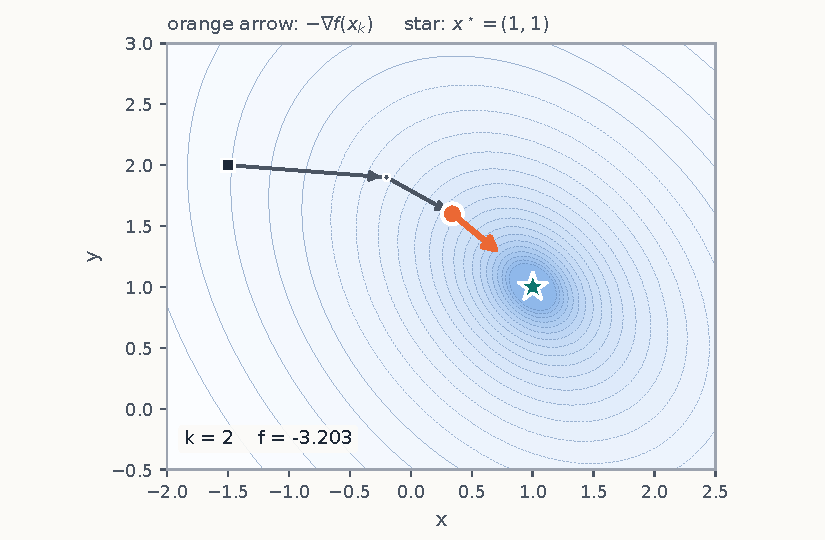
\includegraphics[height=0.70\textheight]{fig_gd_frame_2}}%
      \only<4>{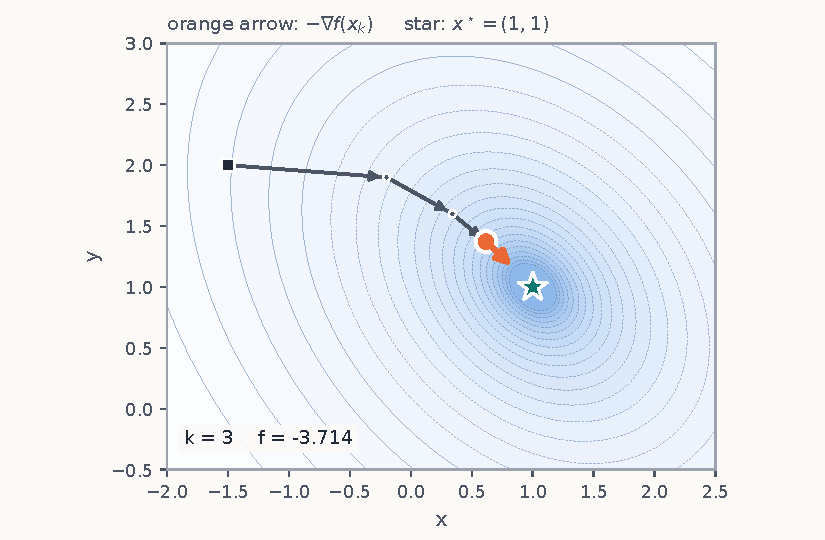
\includegraphics[height=0.70\textheight]{fig_gd_frame_3}}%
      \only<5>{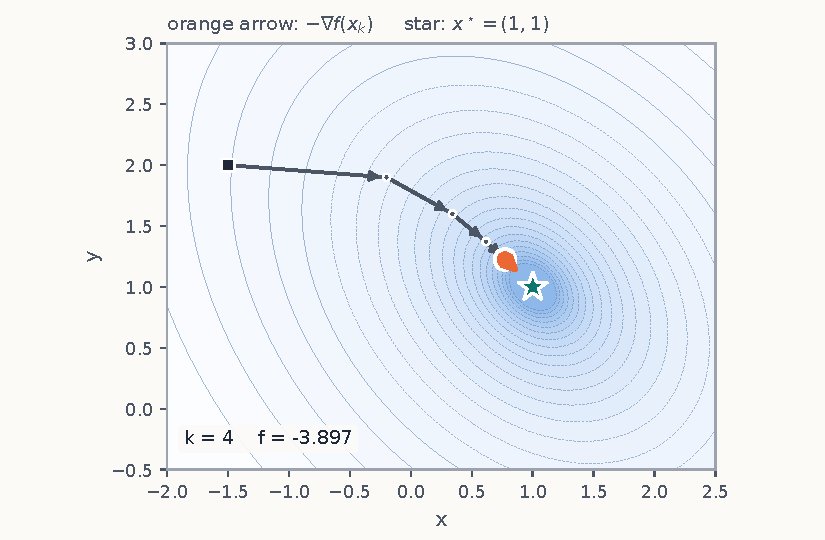
\includegraphics[height=0.70\textheight]{fig_gd_frame_4}}%
      \only<6>{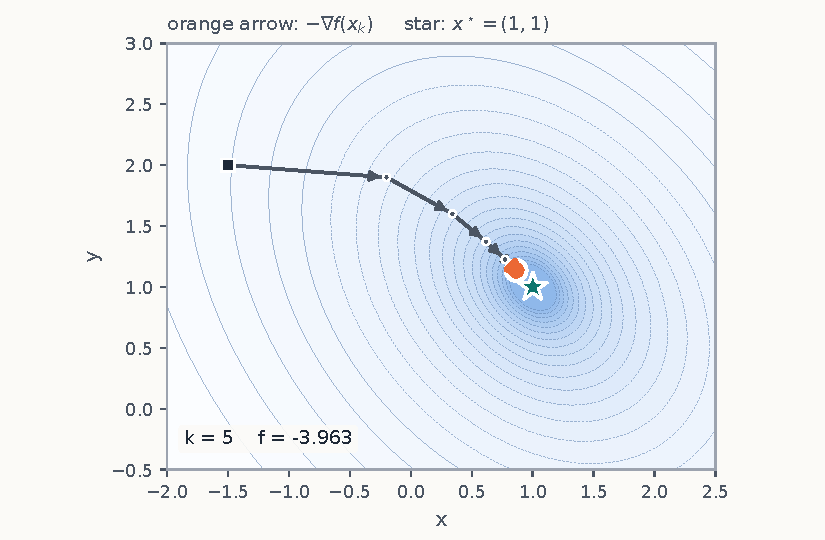
\includegraphics[height=0.70\textheight]{fig_gd_frame_5}}%
      \only<7>{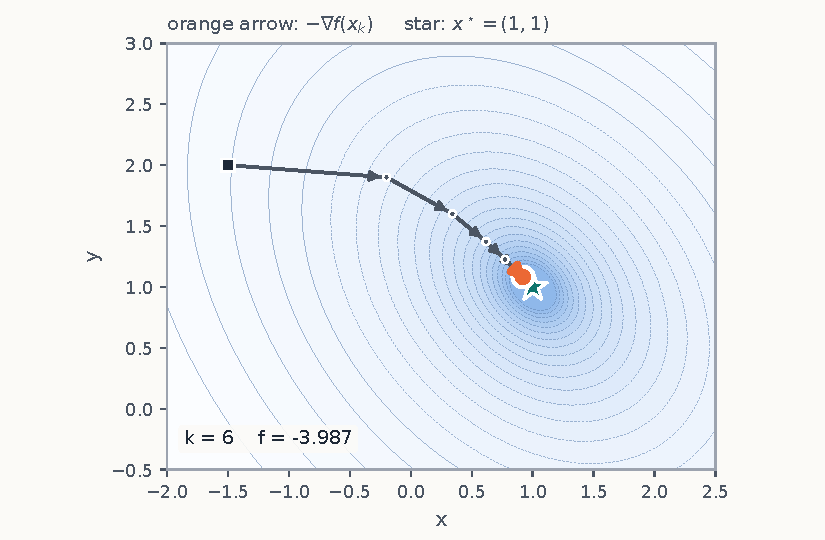
\includegraphics[height=0.70\textheight]{fig_gd_frame_6}}%
      \only<8>{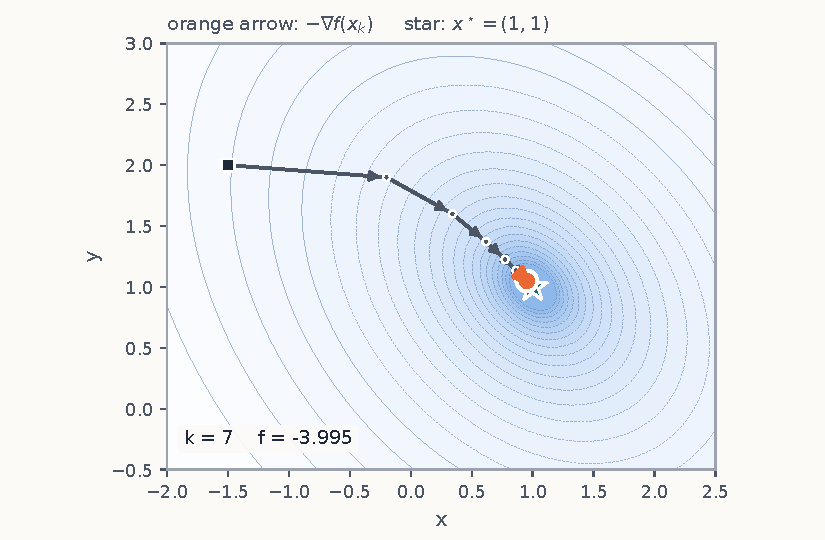
\includegraphics[height=0.70\textheight]{fig_gd_frame_7}}%
    \end{column}
    \begin{column}{0.36\textwidth}
      \footnotesize
      The M3 quadratic, $\bA = \bigl(\begin{smallmatrix}3&1\\1&3\end{smallmatrix}\bigr)$, $\vb = (4,4)$,
      from $\x_0 = (-1.5,2)$, $\alpha = 0.2$.
      \begin{itemize}\footnotesize
        \item<1-> The orange arrow, $-\nabla f(\x_k)$, leaves at a right angle to the contour.
        \item<2-> The first step is long: $\norm{\nabla f}$ is big out here.
        \item<4-> The steps shrink on their own as $\nabla f\to\mathbf 0$, with $\alpha$ fixed.
        \item<6-> The path bends: on ellipses, $-\nabla f$ misses $\x^\star$.
        \item<8-> After 7 steps $f = -3.995$; the optimum is $-4$.
      \end{itemize}
    \end{column}
  \end{columns}
\end{frame}

\begin{frame}{The same descent on the line fit}
  \centering
  \only<1>{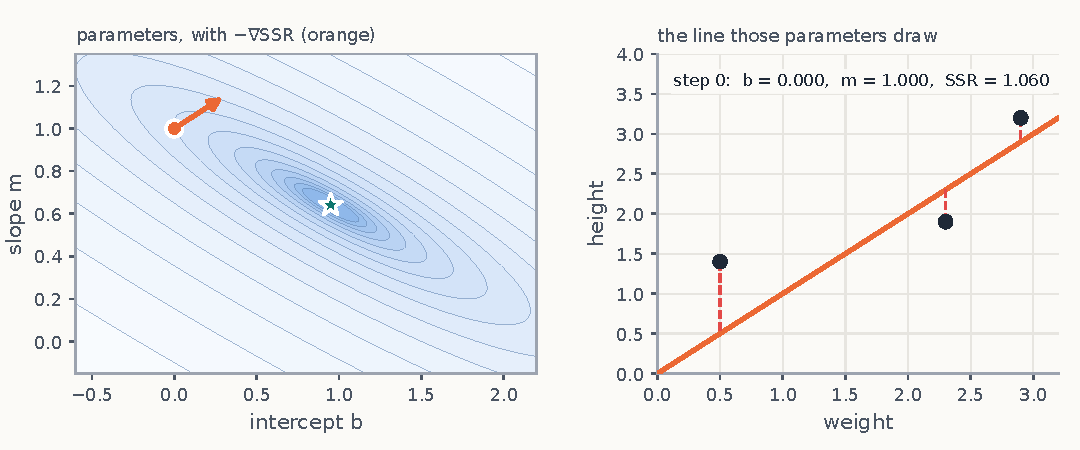
\includegraphics[width=\textwidth, height=0.6\textheight, keepaspectratio]{fig_ssr_frame_0}}%
  \only<2>{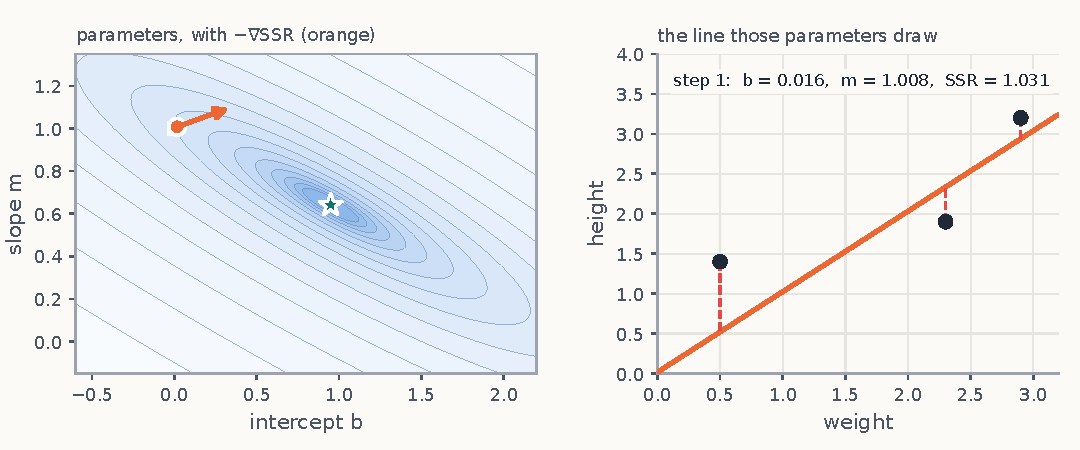
\includegraphics[width=\textwidth, height=0.6\textheight, keepaspectratio]{fig_ssr_frame_1}}%
  \only<3>{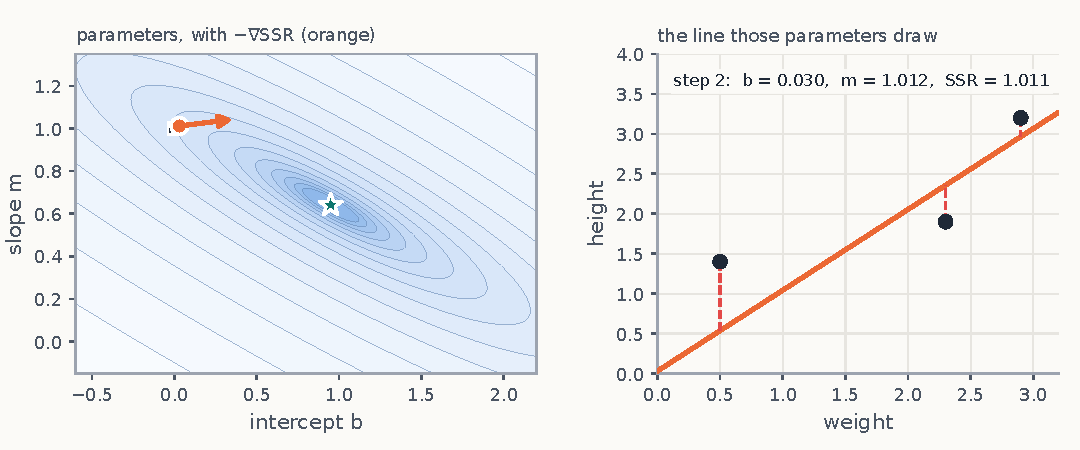
\includegraphics[width=\textwidth, height=0.6\textheight, keepaspectratio]{fig_ssr_frame_2}}%
  \only<4>{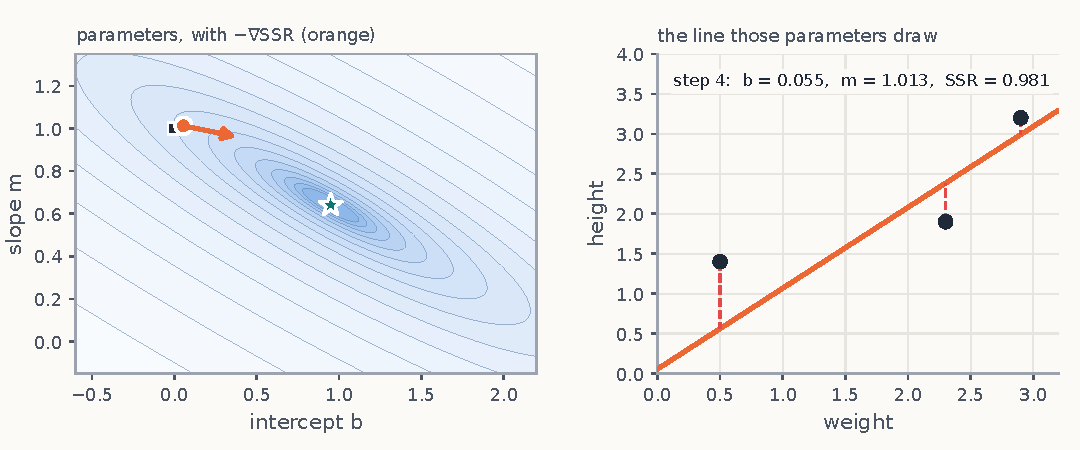
\includegraphics[width=\textwidth, height=0.6\textheight, keepaspectratio]{fig_ssr_frame_3}}%
  \only<5>{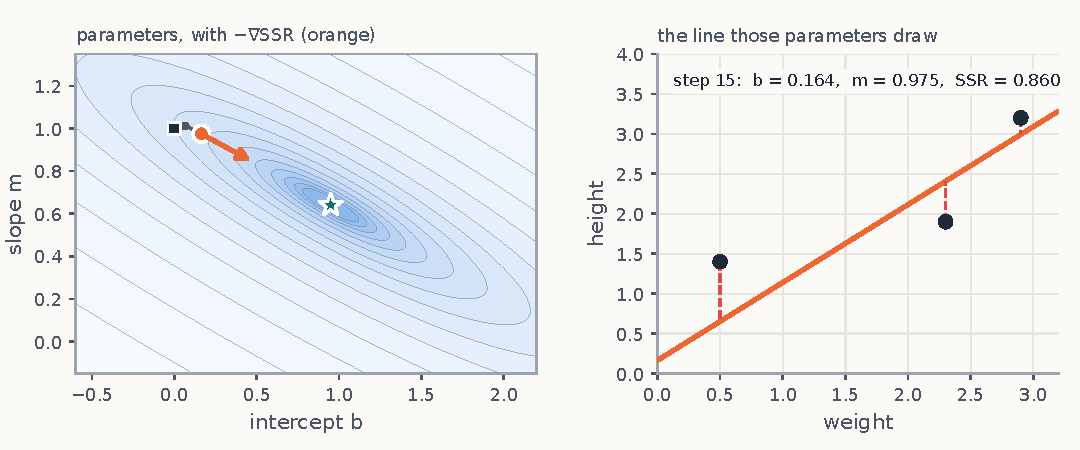
\includegraphics[width=\textwidth, height=0.6\textheight, keepaspectratio]{fig_ssr_frame_4}}%
  \only<6>{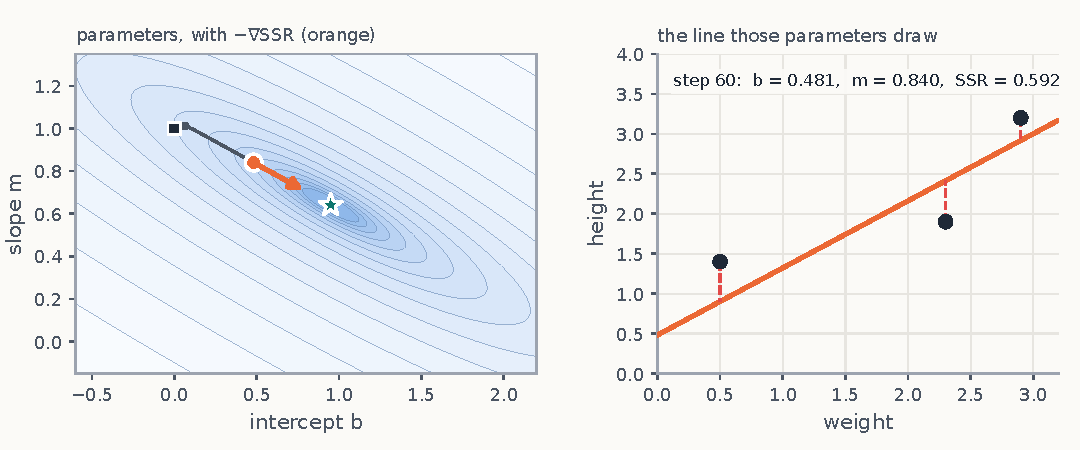
\includegraphics[width=\textwidth, height=0.6\textheight, keepaspectratio]{fig_ssr_frame_5}}%
  \only<7>{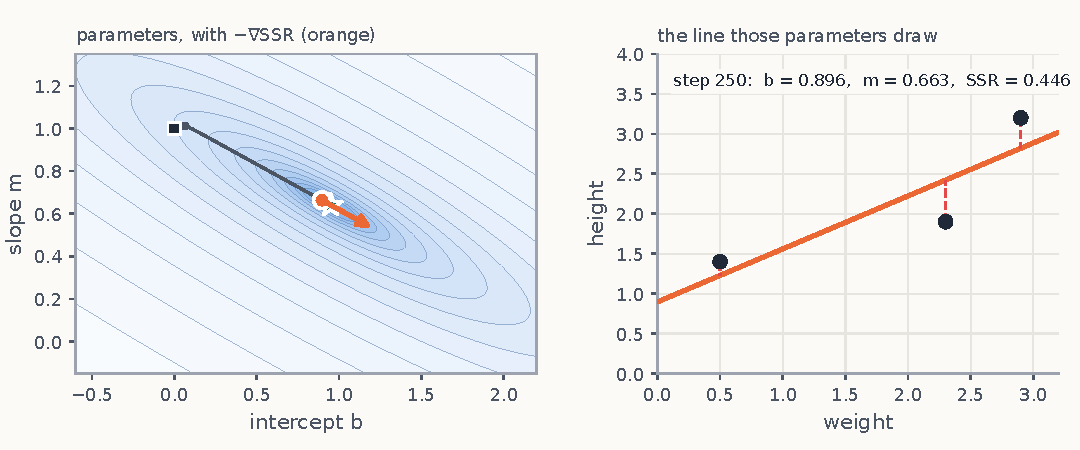
\includegraphics[width=\textwidth, height=0.6\textheight, keepaspectratio]{fig_ssr_frame_6}}%
  \only<8>{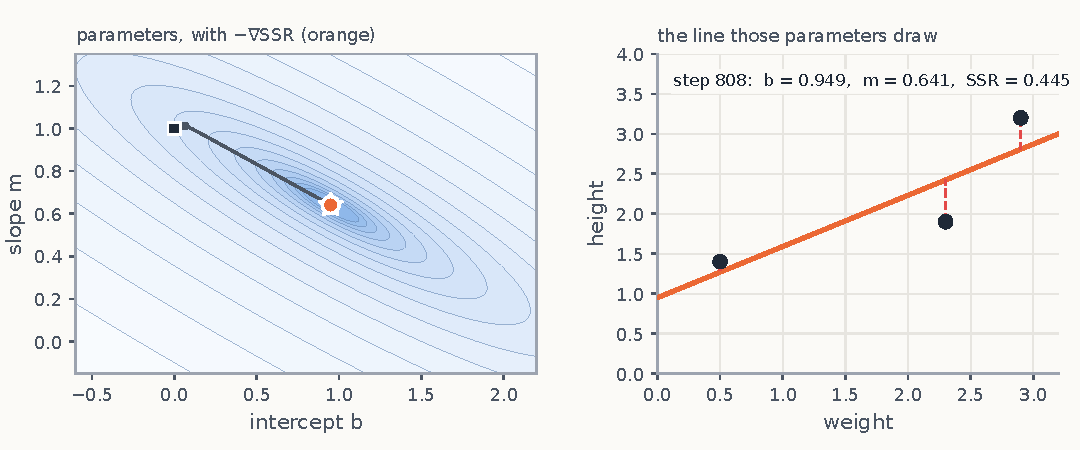
\includegraphics[width=\textwidth, height=0.6\textheight, keepaspectratio]{fig_ssr_frame_7}}%

  \raggedright\footnotesize
  The weight--height data of Section 1, both parameters free, $\alpha = 0.01$ from $(b, m) = (0, 1)$.
  Left: the point $(b, m)$ walks downhill across the SSR contours. Right: the line that point draws.
  Click through steps $0, 1, 2, 4, 15, 60, 250, 808$.
\end{frame}

\begin{frame}{The same walk on the SSR surface}
  \begin{columns}[T]
    \begin{column}{0.56\textwidth}
      \centering
      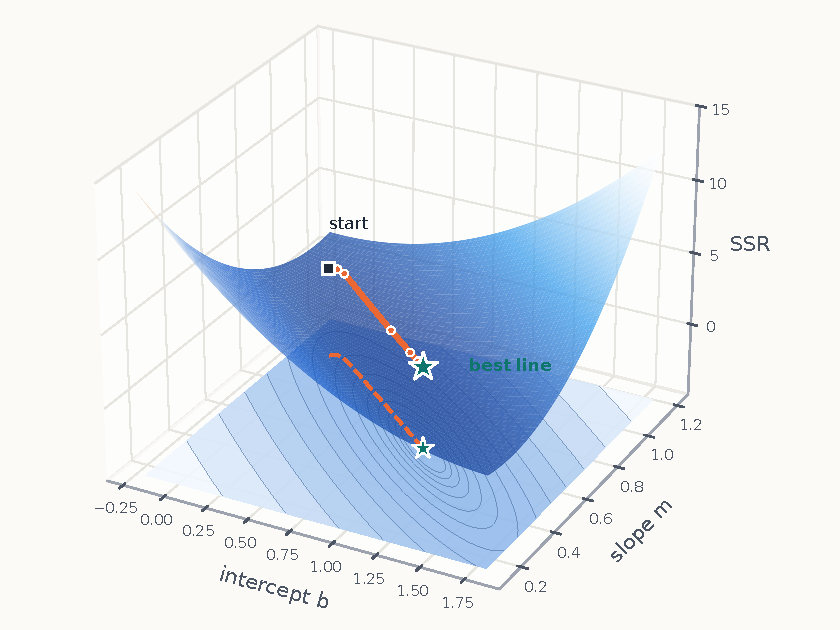
\includegraphics[width=\linewidth, height=0.76\textheight, keepaspectratio]{fig_ssr_surface}
    \end{column}
    \begin{column}{0.42\textwidth}
      \small
      $\SSR(b, m)$ is a bowl over the $(b, m)$ plane. Every point of the bowl is one line through the data.
      \begin{itemize}\footnotesize
        \item GD starts at $(0, 1)$ and rolls downhill. The dashed curve is its shadow on the contour map,
              the path of the previous slide.
        \item It drops into the valley in a few steps, then creeps along the valley floor, because the valley
              is long and narrow ($\kappa \approx 29$, see Section 8).
        \item After $808$ steps it stops at $(0.9486,\ 0.6411)$, the least-squares line $(0.9487,\ 0.6410)$.
      \end{itemize}
    \end{column}
  \end{columns}
\end{frame}

\begin{frame}{Round bowls are easy, long valleys are not}
  \centering
  % Round vs elongated contours: -grad points at the minimiser only for round ones
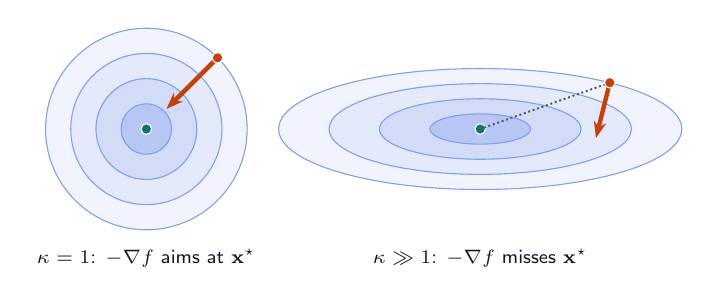
\begin{tikzpicture}[scale=0.8, >={Stealth[length=6pt]}]
  % round bowl
  \begin{scope}
    \foreach \r/\c in {1.6/6, 1.2/12, 0.8/20, 0.4/32}
      \fill[mBlue!\c] (0,0) circle (\r);
    \foreach \r in {0.4,0.8,1.2,1.6} \draw[mBlue!55, line width=0.4pt] (0,0) circle (\r);
    \fill[mGreen, draw=white] (0,0) circle (2.4pt);
    \draw[->, line width=1.6pt, mOrange] (1.13,1.13) -- (0.32,0.32);
    \fill[mOrange, draw=white] (1.13,1.13) circle (2.4pt);
    \node[font=\scriptsize, mInk, align=center] at (0,-2.05) {$\kappa = 1$: $-\nabla f$ aims at $\x^\star$};
  \end{scope}
  % elongated bowl  (semi-axes 2s and 0.6s)
  \begin{scope}[xshift=5.3cm]
    \foreach \s/\c in {1.6/6, 1.2/12, 0.8/20, 0.4/32}
      \fill[mBlue!\c] (0,0) ellipse ({2*\s} and {0.6*\s});
    \foreach \s in {0.4,0.8,1.2,1.6} \draw[mBlue!55, line width=0.4pt] (0,0) ellipse ({2*\s} and {0.6*\s});
    \fill[mGreen, draw=white] (0,0) circle (2.4pt);
    % point on the outer ellipse at parameter 50 degrees: (2.057, 0.735)
    \draw[mGrey, densely dotted, line width=0.7pt] (2.057,0.735) -- (0,0);
    \draw[->, line width=1.6pt, mOrange] (2.057,0.735) -- ++(-0.22,-0.88);
    \fill[mOrange, draw=white] (2.057,0.735) circle (2.4pt);
    \node[font=\scriptsize, mInk, align=center] at (0,-2.05) {$\kappa \gg 1$: $-\nabla f$ misses $\x^\star$};
  \end{scope}
\end{tikzpicture}


  \vspace{4pt}
  \raggedright
  \begin{itemize}\small
    \item \textbf{Round contours} ($\bA\propto\bI$): $-\nabla f$ points straight at $\x^\star$; one well-chosen step lands on it.
    \item \textbf{Stretched contours}: $-\nabla f$ is still perpendicular to the contour, so it \emph{misses} $\x^\star$.
          The iterates bounce across the valley and crawl along it.
    \item How stretched is measured by the \alert{condition number} $\kappa = \lmax/\lmin$. It returns in the step limit (Section~5),
          every rate (Section~7) and the zig-zag (Section~8).
  \end{itemize}
\end{frame}

% =====================================================================
%  5. Step-size analysis and stability
% =====================================================================
\section{How big a step can we take?}

\begin{frame}{Start with quadratics, where everything is exact}
  Take $f(\x) = \tfrac12\x\T\bA\x - \vb\T\x$ with $\bA\succ0$ symmetric, so $\nabla f = \bA\x - \vb$ and $\bA\x^\star = \vb$. Then
  \[
    \e_{k+1} = \x_{k+1} - \x^\star = (\bI - \alpha\bA)\,\e_k \;\Longrightarrow\; \e_k = (\bI-\alpha\bA)^k\e_0 .
  \]
  Diagonalise $\bA = \mathbf Q\boldsymbol\Lambda\mathbf Q\T$ and write $\mathbf z_k = \mathbf Q\T\e_k$. The coupled iteration
  \alert{falls apart into $n$ independent scalar ones}:
  \[
    z_i^{(k)} = (1 - \alpha\lambda_i)^k\, z_i^{(0)}, \qquad i = 1,\dots,n .
  \]
  \begin{keybox}[Why bother with quadratics?]
    Close to a strict minimiser, $f(\x)\approx f(\x^\star) + \tfrac12(\x-\x^\star)\T\nabla^2 f(\x^\star)(\x-\x^\star)$.
    So the quadratic analysis with $\bA = \nabla^2 f(\x^\star)$ predicts how GD behaves \emph{near the end}
    on any smooth $f$ (Problem M1(d) uses exactly this).
  \end{keybox}
\end{frame}

\begin{frame}{Theorem: the stable window and the best fixed step}
  \begin{columns}[T]
    \begin{column}{0.52\textwidth}
      \begin{thmbox}[Theorem]
        \small
        GD converges from every $\x_0$ iff $0 < \alpha < 2/\lmax$, at rate
        \[
          \rho(\alpha) = \max\bigl\{|1-\alpha\lmin|,\ |1-\alpha\lmax|\bigr\}.
        \]
        The best choice is $\alpha^\star = \frac{2}{\lmin+\lmax}$, giving $\rho^\star = \frac{\kappa-1}{\kappa+1}$ with $\kappa = \frac{\lmax}{\lmin}$.
      \end{thmbox}
      \footnotesize\textbf{Proof.} $|1-\alpha\lambda|$ is convex in $\lambda$, so its maximum over $[\lmin,\lmax]$ sits at an end.
      Both ends are below 1 iff $\alpha<2/\lmax$. The best $\alpha$ makes the two ends equal: $1-\alpha\lmin = \alpha\lmax - 1$. $\blacksquare$
    \end{column}
    \begin{column}{0.46\textwidth}
      \centering
      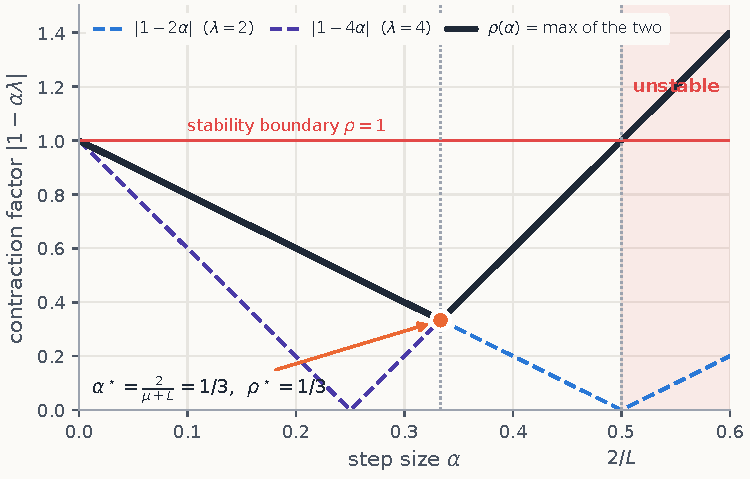
\includegraphics[width=\linewidth]{fig_amplification}

      \vspace{2pt}
      \footnotesize To reach accuracy $\varepsilon$ you need about $\frac{\kappa+1}{2}\ln\frac1\varepsilon$ steps, i.e.\ $O\!\bigl(\kappa\log\tfrac1\varepsilon\bigr)$.
    \end{column}
  \end{columns}
\end{frame}

\begin{frame}{Same problem, four step sizes}
  \begin{columns}[T]
    \begin{column}{0.6\textwidth}
      \centering
      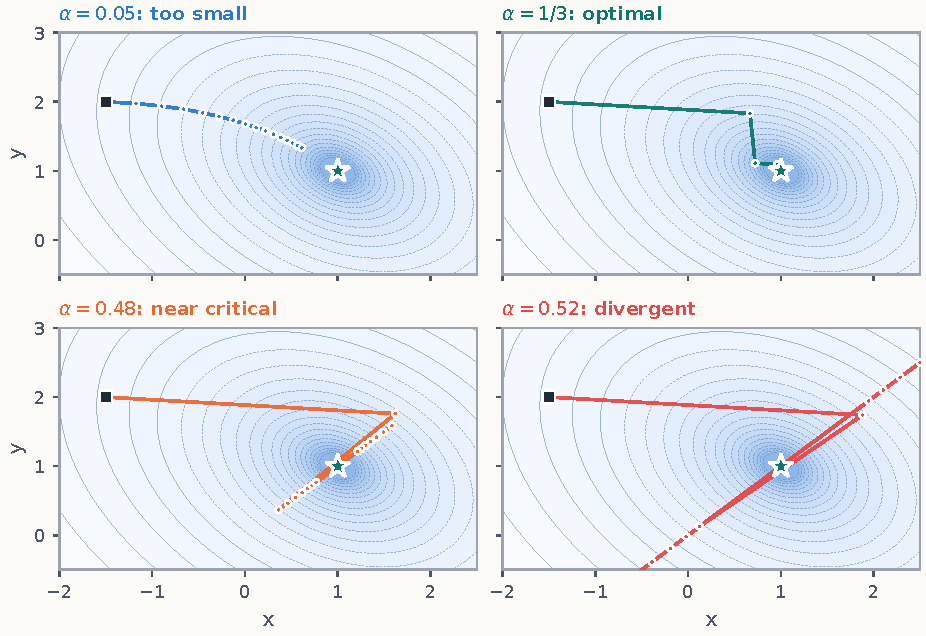
\includegraphics[width=\linewidth,height=0.80\textheight,keepaspectratio]{fig_stepsize_compare}
    \end{column}
    \begin{column}{0.38\textwidth}
      \small
      $\lambda(\bA)\in\{2,4\}$, so GD is stable only for $\alpha<0.5$.
      \begin{itemize}\footnotesize
        \item $\alpha=0.05$: $\rho = 0.9$. It gets there, eventually.
        \item $\alpha = \tfrac13$: $\rho = \tfrac13$, the M3 optimum.
        \item $\alpha = 0.48$: $|1-4\alpha| = 0.92$, rattling across the valley.
        \item $\alpha = 0.52$: $|1-4\alpha| = 1.08$, and the swings grow without bound.
      \end{itemize}
      \footnotesize\textcolor{mGrey}{Too small wastes time; too large wrecks the run.}
    \end{column}
  \end{columns}
\end{frame}

\begin{frame}{Seen from numerical ODEs: Euler's stability region}
  \begin{columns}[T]
    \begin{column}{0.5\textwidth}
      \small
      For a quadratic the gradient flow is $\dot\e = -\bA\e$, so each mode is the Dahlquist test equation
      $\dot y = \lambda y$ with $\lambda = -\lambda_i < 0$.
      \begin{itemize}\footnotesize
        \item The \textbf{exact flow} decays for every $\lambda_i>0$. Nothing can go wrong in continuous time.
        \item \textbf{Forward Euler} is stable only when $z = h\lambda$ lies in the disk $|1+z|<1$.
              Here $z_i = -\alpha\lambda_i$, so we need $0<\alpha\lambda_i<2$, which is exactly $\alpha<2/\lmax$.
        \item This is \textbf{stiffness}: the \emph{fastest} mode ($\lmax$) limits the step, while the \emph{slowest}
              ($\lmin$) decides how long you wait. Any explicit scheme pays roughly $\kappa$ steps.
      \end{itemize}
    \end{column}
    \begin{column}{0.48\textwidth}
      \centering
      % Explicit-Euler stability disk |1 + z| < 1 with the points z_i = -alpha*lambda_i
% (Problem M3: lambda = 2, 4) for alpha = 1/3 (stable) and alpha = 0.6 (unstable)
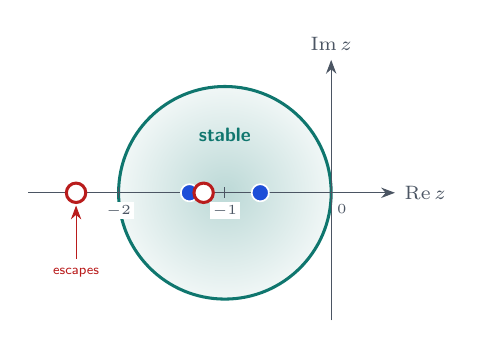
\begin{tikzpicture}[scale=1.35, >={Stealth[length=5pt]}]
  \shade[inner color=mGreen!28, outer color=mGreen!6] (-1,0) circle (1);
  \draw[line width=1.1pt, mGreen] (-1,0) circle (1);
  % axes
  \draw[->, mGrey] (-2.85,0) -- (0.6,0) node[right, font=\scriptsize] {$\mathrm{Re}\,z$};
  \draw[->, mGrey] (0,-1.2) -- (0,1.25) node[above, font=\scriptsize] {$\mathrm{Im}\,z$};
  \foreach \t/\lab in {-2/-2, -1/-1} {
    \draw[mGrey] (\t,0.05) -- (\t,-0.05);
    \node[font=\tiny, mGrey, fill=white, inner sep=1pt] at (\t,-0.17) {$\lab$};
  }
  \node[font=\tiny, mGrey] at (0.1,-0.15) {$0$};
  \node[font=\scriptsize\bfseries, mGreen] at (-1,0.55) {stable};
  % alpha = 1/3: z = -2/3, -4/3
  \fill[mBlue, draw=white, line width=0.6pt] (-0.667,0) circle (2.3pt);
  \fill[mBlue, draw=white, line width=0.6pt] (-1.333,0) circle (2.3pt);
  % alpha = 0.6: z = -1.2, -2.4
  \draw[mRed, line width=1.1pt, fill=white] (-1.2,0) circle (2.6pt);
  \draw[mRed, line width=1.1pt, fill=white] (-2.4,0) circle (2.6pt);
  \draw[mRed, ->] (-2.4,-0.62) node[below, font=\tiny] {escapes} -- (-2.4,-0.12);
\end{tikzpicture}


      \footnotesize
      \textcolor{mBlue}{$\bullet$} $\alpha = \frac13$: $z = -\frac23, -\frac43$, both inside.\quad
      \textcolor{mRed}{$\circ$} $\alpha = 0.6$: $z = -1.2, -2.4$, one escapes.

      \vspace{2pt}
      Backward Euler, $\x_{k+1} = \x_k - h\nabla f(\x_{k+1})$, is stable for every $h$.
      That is the proximal-point method; the catch is that each step is itself an optimisation problem.
    \end{column}
  \end{columns}
\end{frame}

% =====================================================================
%  6. Function classes: smoothness, convexity, strong convexity
% =====================================================================
\section{What we need to assume about $f$}

\begin{frame}{Three assumptions, and which functions satisfy them}
  \small
  \begin{tabular}{@{}p{2.6cm} p{5.2cm} p{3.6cm}@{}}
    \toprule
    Property & Definition & If $f\in C^2$ \\
    \midrule
    $L$-smooth & $\norm{\nabla f(\x)-\nabla f(\y)}\le L\norm{\x-\y}$ & $-L\bI\preceq\nabla^2f\preceq L\bI$ \\[3pt]
    convex & $f(\y)\ge f(\x)+\nabla f(\x)\T(\y-\x)$ & $\nabla^2 f\succeq 0$ \\[3pt]
    $\mu$-strongly convex & $f(\y)\ge f(\x)+\nabla f(\x)\T(\y-\x)+\tfrac\mu2\norm{\y-\x}^2$ & $\nabla^2 f\succeq\mu\bI$ \\
    \bottomrule
  \end{tabular}

  \vspace{6pt}
  \begin{tabular}{@{}l c c c@{}}
    \toprule
    Example & $L$-smooth? & convex? & strongly convex? \\
    \midrule
    $\tfrac12\x\T\bA\x - \vb\T\x$, $\bA\succ0$ & \checkmark\ $L=\lmax$ & \checkmark & \checkmark\ $\mu=\lmin$ \\
    logistic loss $\log(1+e^{-y\,\mathbf a\T\x})$ & \checkmark & \checkmark & $\times$ \\
    $x^4$ & $\times$ (not globally) & \checkmark & $\times$ (flat at 0) \\
    $x^4+y^4-4xy$ (M1) & $\times$ (not globally) & $\times$ & $\times$ \\
    \bottomrule
  \end{tabular}
\end{frame}

\begin{frame}{Squeezed between two parabolas}
  \begin{columns}[T]
    \begin{column}{0.5\textwidth}
      \centering
      % Quadratic sandwich: mu-strong convexity (lower) and L-smoothness (upper) at x.
% f(y) = 0.5 y^2 + 0.6 log(cosh(1.5 y)), so f'' lies in [1, 1 + 1.35] = [1, 2.35]
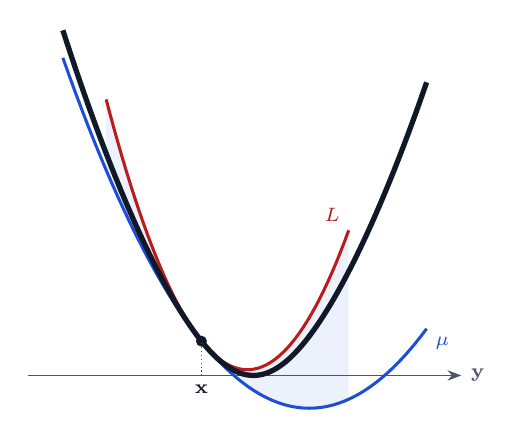
\begin{tikzpicture}[scale=1.1, >={Stealth[length=5pt]},
  declare function={
    lc(\y)=ln(cosh(1.5*\y));
    f(\y)=0.5*\y*\y + 0.6*lc(\y);
    fp(\y)=\y + 0.9*tanh(1.5*\y);
    up(\y)=f(-0.6) + fp(-0.6)*(\y+0.6) + 0.5*2.35*(\y+0.6)*(\y+0.6);
    lo(\y)=f(-0.6) + fp(-0.6)*(\y+0.6) + 0.5*1.0*(\y+0.6)*(\y+0.6);}]
  % the corridor where f must live
  \fill[mBlue!8, domain=-1.7:1.1, samples=60]
    plot (\x, {up(\x)}) -- plot[domain=1.1:-1.7, samples=60] (\x, {lo(\x)}) -- cycle;
  \draw[->, mGrey] (-2.6,0) -- (2.4,0) node[right, font=\scriptsize] {$\y$};
  \draw[line width=1.1pt, mRed, domain=-1.7:1.1, samples=60] plot (\x, {up(\x)});
  \draw[line width=1.1pt, mBlue, domain=-2.2:2.0, samples=60] plot (\x, {lo(\x)});
  \draw[line width=1.9pt, mInk, domain=-2.2:2.0, samples=100] plot (\x, {f(\x)});
  \fill[mInk] (-0.6,{f(-0.6)}) circle (1.8pt);
  \draw[mGrey, densely dotted] (-0.6,0) node[below, font=\scriptsize, mInk] {$\x$} -- (-0.6,{f(-0.6)});
  \node[font=\scriptsize, mRed, anchor=south east, inner sep=3pt] at (1.1,{up(1.1)}) {$L$};
  \node[font=\scriptsize, mBlue, anchor=north west, inner sep=3pt] at (2.0,{lo(2.0)}) {$\mu$};
\end{tikzpicture}


      \scriptsize
      \textcolor{mRed}{\rule[2pt]{10pt}{1.1pt}} upper, curvature $L$ \quad
      \textcolor{mInk}{\rule[2pt]{10pt}{1.8pt}} $f$ \quad
      \textcolor{mBlue}{\rule[2pt]{10pt}{1.1pt}} lower, curvature $\mu$
    \end{column}
    \begin{column}{0.48\textwidth}
      \small
      If $f$ is $L$-smooth and $\mu$-strongly convex, then at every point it lives inside the shaded corridor
      between two parabolas.

      \vspace{3pt}
      Minimising the lower parabola over $\y$ gives
      \[
        f^\star \ge f(\x) - \frac{1}{2\mu}\norm{\nabla f(\x)}^2 ,
      \]
      and three useful facts follow:
      \begin{itemize}\footnotesize
        \item The gradient \emph{certifies} how close you are: $f(\x)-f^\star\le\frac{\norm{\nabla f}^2}{2\mu}$ and
              $\norm{\x-\x^\star}\le\frac{\norm{\nabla f(\x)}}{\mu}$.
        \item There is exactly one minimiser.
        \item The upper parabola is where the step $1/L$ comes from (Section~3, View 2).
      \end{itemize}
    \end{column}
  \end{columns}
\end{frame}

\begin{frame}{The condition number $\kappa = L/\mu$}
  \begin{itemize}\small
    \item $\kappa\ge1$ compares the steepest curvature with the flattest. For a quadratic, the contour ellipses
          are $\sqrt\kappa$ times longer than they are wide.
    \item Keep an eye on it: $\kappa$ shows up in \emph{every} rate from here on. GD needs $O(\kappa\log\frac1\varepsilon)$ iterations,
          accelerated methods $O(\sqrt\kappa\log\frac1\varepsilon)$.
  \end{itemize}
  \vspace{2pt}
  \centering\small
  \begin{tabular}{@{}l c l@{}}
    \toprule
    Problem & $\kappa$ & Where the ill-conditioning comes from \\
    \midrule
    M3 quadratic & $2$ & nowhere, it is a friendly problem \\
    A1 regression, raw feature & $46.1$ & the columns $[x,\mathbf 1]$ are correlated \\
    A1 after centring & $1.5$ & preprocessing removed it \\
    A2 spring chain, $k_1 = 1000$ & $1002$ & one very stiff member next to a soft one \\
    Rosenbrock at $(1,1)$ & $\approx2508$ & curved valley ($\lambda = 1001.6,\ 0.399$) \\
    \bottomrule
  \end{tabular}
\end{frame}

% =====================================================================
%  7. Convergence analysis
% =====================================================================
\section{How fast does it converge?}

\begin{frame}{One inequality drives every proof}
  \begin{thmbox}[Descent lemma (proved in full in Problem M2)]
    If $\nabla f$ is $L$-Lipschitz: $\;f(\y)\le f(\x)+\nabla f(\x)\T(\y-\x)+\tfrac L2\norm{\y-\x}^2$.
  \end{thmbox}
  \small
  \textbf{Proof idea.}
  \pause
  $f(\y)-f(\x)-\nabla f(\x)\T(\y-\x) = \int_0^1[\nabla f(\x+t(\y-\x))-\nabla f(\x)]\T(\y-\x)\,dt$,
  \pause
  and Cauchy--Schwarz with the Lipschitz bound turns this into $\le\int_0^1 Lt\norm{\y-\x}^2dt = \tfrac L2\norm{\y-\x}^2$. $\blacksquare$

  \pause
  \vspace{4pt}
  \normalsize Plug in $\y = \x_k - \alpha\g_k$:
  \[
    f(\x_{k+1}) \le f(\x_k) - \alpha\Bigl(1 - \frac{\alpha L}2\Bigr)\norm{\g_k}^2
    \;\overset{\alpha = 1/L}{=}\; f(\x_k) - \frac{1}{2L}\norm{\g_k}^2 .
  \]
  \small Each step buys a guaranteed drop of $\norm{\g_k}^2/(2L)$. Every rate that follows comes from linking
  $\norm{\g_k}$ to how far we still are from the optimum.
\end{frame}

\begin{frame}{No convexity: we can only promise a small gradient}
  \begin{thmbox}[Theorem ($L$-smooth, bounded below, $\alpha = 1/L$)]
    \[
      \min_{0\le k<K}\norm{\nabla f(\x_k)} \le \sqrt{\frac{2L\,(f(\x_0)-f^\star)}{K}} = O\!\bigl(1/\sqrt K\bigr).
    \]
  \end{thmbox}
  \small\textbf{Proof.} Add up the per-step drops for $k = 0,\dots,K-1$. The total cannot exceed
  $f(\x_0) - f(\x_K)\le f(\x_0)-f^\star$ (details in Problem M2). $\blacksquare$
  \begin{itemize}\small
    \item All we get is a point with a \emph{small gradient}. It could be a saddle or a poor local minimum.
    \item Reaching $\norm{\nabla f}\le\varepsilon$ takes $O(L(f_0-f^\star)/\varepsilon^2)$ iterations, which is slow.
          That is what you pay for assuming nothing.
    \item Deep learning lives here. The faster rates on the next slides all need extra structure.
  \end{itemize}
\end{frame}

\begin{frame}{Convex functions: error $O(1/k)$}
  \begin{thmbox}[Theorem ($L$-smooth, convex, $\alpha = 1/L$)]
    \[ f(\x_k) - f^\star \le \frac{L\norm{\x_0-\x^\star}^2}{2k}. \]
  \end{thmbox}
  \small\textbf{Proof.}
  \pause
  Convexity gives $f(\x_k)\le f^\star + \g_k\T(\x_k-\x^\star)$. Combine that with the guaranteed drop:
  \[
    f(\x_{k+1}) - f^\star \le \g_k\T(\x_k-\x^\star) - \tfrac{1}{2L}\norm{\g_k}^2
    = \tfrac L2\Bigl(\norm{\x_k-\x^\star}^2 - \norm{\x_{k+1}-\x^\star}^2\Bigr).
  \]
  \pause
  (The equality is just $\norm{\x_k - \x^\star - \g_k/L}^2$ expanded.) Summing over $k = 0,\dots,K-1$, the right side
  telescopes:
  \[
    \textstyle\sum_{k=1}^{K}\bigl(f(\x_k)-f^\star\bigr)\le\tfrac L2\norm{\x_0-\x^\star}^2 .
  \]
  \pause
  The values $f(\x_k)$ never increase, so the left side is at least $K\bigl(f(\x_K)-f^\star\bigr)$. $\blacksquare$
\end{frame}

\begin{frame}{Strongly convex functions: the error shrinks geometrically}
  \begin{thmbox}[Theorem ($L$-smooth, $\mu$-strongly convex, $\alpha = 1/L$)]
    \[ \norm{\x_{k}-\x^\star}^2 \le \Bigl(1-\frac{\mu}{L}\Bigr)^{k}\norm{\x_0-\x^\star}^2 = \Bigl(1-\frac1\kappa\Bigr)^k\norm{\x_0-\x^\star}^2. \]
  \end{thmbox}
  \small\textbf{Proof.} Write $\e = \x_k-\x^\star$, $\Delta = f(\x_k)-f^\star$, and expand
  $\norm{\x_{k+1}-\x^\star}^2 = \norm{\e}^2 - \tfrac2L\g_k\T\e + \tfrac1{L^2}\norm{\g_k}^2$. Two facts bound the middle and last terms:
  \pause
  \begin{itemize}\footnotesize
    \item strong convexity at $\y=\x^\star$: $\;\g_k\T\e\ge\Delta+\tfrac\mu2\norm{\e}^2$;
    \item the descent lemma at $\x_k-\g_k/L$: $\;f^\star\le f(\x_k)-\tfrac1{2L}\norm{\g_k}^2$, i.e. $\norm{\g_k}^2\le2L\Delta$.
  \end{itemize}
  \pause
  \[
    \norm{\x_{k+1}-\x^\star}^2\le\norm{\e}^2-\tfrac2L\Delta-\tfrac\mu L\norm{\e}^2+\tfrac2L\Delta
    =\Bigl(1-\tfrac\mu L\Bigr)\norm{\e}^2. \quad\blacksquare
  \]
  \pause
  \footnotesize With $\alpha = \frac{2}{\mu+L}$ the factor improves to $\norm{\e_{k+1}}\le\frac{\kappa-1}{\kappa+1}\norm{\e_k}$,
  the same number the quadratic analysis gave in Section~5~\cite{nesterov2018}.
\end{frame}

\begin{frame}{Linear rates without convexity: the Polyak--{\L}ojasiewicz condition}
  \begin{thmbox}[PL inequality \normalfont\cite{karimi2016}]
    $\tfrac12\norm{\nabla f(\x)}^2\ge\mu\,(f(\x)-f^\star)$ for all $\x$. Then GD with $\alpha = 1/L$ satisfies
    \[ f(\x_k)-f^\star\le\Bigl(1-\frac\mu L\Bigr)^k\bigl(f(\x_0)-f^\star\bigr). \]
  \end{thmbox}
  \small\textbf{Proof (two lines).}
  $f(\x_{k+1})-f^\star\le f(\x_k)-f^\star-\tfrac1{2L}\norm{\g_k}^2\le\bigl(1-\tfrac\mu L\bigr)(f(\x_k)-f^\star)$. $\blacksquare$
  \begin{itemize}\small
    \item PL does \emph{not} need convexity. $f(x) = x^2+3\sin^2x$ has $f''$ dipping to $-4$,
          yet it satisfies PL (numerically $\mu\approx0.175$).
    \item Strong convexity implies PL (from the Section~6 sandwich), so PL is the more general route to a linear rate.
    \item Least squares $\tfrac12\norm{\mathbf M\x-\vb}^2$ with a rank-deficient $\mathbf M$ is convex but not strongly convex.
          It still satisfies PL, so GD still converges linearly in $f$~\cite{karimi2016}.
  \end{itemize}
\end{frame}

\begin{frame}{Order of convergence, and the scorecard so far}
  \begin{columns}[T]
    \begin{column}{0.55\textwidth}
      \small
      A sequence $\{\e_k\}$ has \textbf{order $p$} if $\norm{\e_{k+1}}\approx r\norm{\e_k}^p$.
      \begin{itemize}\footnotesize
        \item GD has $p = 1$, \alert{linear} order, with $r\le\rho$. It gains the \emph{same} number of correct digits,
              $-\log_{10}\rho$, every step.
        \item In the plot, $\log e_{k+1}$ against $\log e_k$ is a line of slope 1. The dashed slope-2 line
              (quadratic order, as in Newton-type methods) is there for comparison.
      \end{itemize}
      \vspace{2pt}
      \footnotesize
      \begin{tabular}{@{}l l l@{}}
        \toprule
        Setting & Guarantee ($\alpha = \frac1L$) & Iterations \\
        \midrule
        nonconvex & $\min\norm{\g}^2\le\frac{2L\Delta_0}{K}$ & $O(\varepsilon^{-2})$ \\
        convex & $f-f^\star\le\frac{LR^2}{2k}$ & $O(\varepsilon^{-1})$ \\
        strongly convex & $\norm{\e_k}^2\le(1-\frac1\kappa)^k R^2$ & $O(\kappa\log\frac1\varepsilon)$ \\
        PL & $f-f^\star\le(1-\frac1\kappa)^k\Delta_0$ & $O(\kappa\log\frac1\varepsilon)$ \\
        \bottomrule
      \end{tabular}
    \end{column}
    \begin{column}{0.43\textwidth}
      \centering
      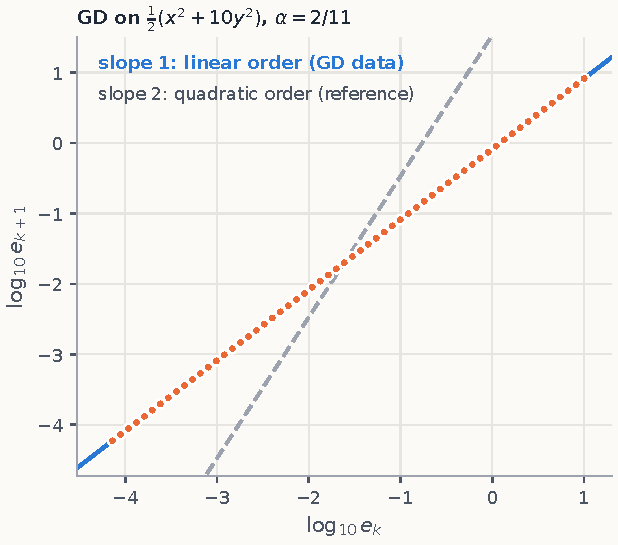
\includegraphics[width=\linewidth]{fig_order}

      \footnotesize\textcolor{mGrey}{$R = \norm{\x_0-\x^\star}$ and $\Delta_0 = f(\x_0)-f^\star$.}
    \end{column}
  \end{columns}
\end{frame}

\begin{frame}{GD or Newton? Count the cost}
  \small
  \emph{When GD, and when Newton?} Count the work for $n$ parameters~\cite{nocedal2006}.

  \vspace{2pt}
  \centering\footnotesize
  \begin{tabular}{@{}l l l@{}}
    \toprule
    & Gradient descent & Newton's method \\
    \midrule
    information used & gradient ($n$ numbers) & gradient + Hessian ($n^2$ numbers) \\
    cost of one step & $O(n)$ after the gradient & $O(n^3)$ to solve $H\mathbf y = \g$ \\
    order of convergence & linear & quadratic \\
    learning rate & must be chosen & not needed \\
    on a concave stretch ($f'' < 0$) & still goes downhill & can head for a \textcolor{mRed}{maximum} \\
    best for & large problems (ML, $n\sim10^6$) & small problems needing high accuracy \\
    \bottomrule
  \end{tabular}

  \raggedright
  \vspace{3pt}
  \begin{keybox}[Why ML uses GD]
    \footnotesize With $n = 10^6$ a Hessian has $10^{12}$ entries and will not fit in memory; GD stores $n$ numbers.
    When $H$ is not positive definite, Levenberg--Marquardt~\cite{nocedal2006} moves towards a gradient step.
  \end{keybox}
\end{frame}

% =====================================================================
%  8. Why convergence can be slow: conditioning and the zig-zag
% =====================================================================
\section{Why it can be so slow: conditioning}

\begin{frame}{What if we pick the perfect step every time?}
  Exact line search takes the \emph{best} step along $-\g_k$: $\;\alpha_k = \argmin_{\alpha>0}f(\x_k-\alpha\g_k)$.
  \begin{itemize}\small
    \item For a quadratic there is a closed form, $\alpha_k = \dfrac{\g_k\T\g_k}{\g_k\T\bA\g_k}$, at the price of one extra matrix--vector product.
    \item For general $f$ it is a 1-D minimisation every iteration. Any 1-D method works (golden-section search, for example,
          which is a separate topic). In practice cheaper inexact rules win (Section~10).
  \end{itemize}
  \begin{thmbox}[Consecutive steps are perpendicular]
    At the optimal $\alpha_k$,
    $\;0 = \tfrac{d}{d\alpha}f(\x_k-\alpha\g_k)\big|_{\alpha_k} = -\nabla f(\x_{k+1})\T\g_k$, so $\;\g_{k+1}\perp\g_k$.
  \end{thmbox}
  \small So every step turns exactly $90^\circ$. In a long narrow valley that produces the famous
  \alert{zig-zag} (Problem M4 proves it and gives the iterates in closed form).
\end{frame}

\begin{frame}{The Kantorovich bound, with a short proof}
  \begin{thmbox}[Theorem (steepest descent with exact line search, quadratic $f$)]
    \[ f(\x_{k+1})-f^\star \le \Bigl(\frac{\kappa-1}{\kappa+1}\Bigr)^2\bigl(f(\x_k)-f^\star\bigr). \]
  \end{thmbox}
  \small\textbf{Proof.}
  \pause
  Shift so that $f - f^\star = \tfrac12\e\T\bA\e = \tfrac12\g\T\bA^{-1}\g$ with $\g = \bA\e$. The exact step gives
  $f(\x_{k+1}) = f(\x_k) - \frac{(\g\T\g)^2}{2\,\g\T\bA\g}$, hence
  \[
    \frac{f(\x_{k+1})-f^\star}{f(\x_k)-f^\star} = 1-\frac{(\g\T\g)^2}{(\g\T\bA\g)(\g\T\bA^{-1}\g)} .
  \]
  \pause
  The \textbf{Kantorovich inequality} says the fraction is at least $\frac{4\lmin\lmax}{(\lmin+\lmax)^2}$, so the ratio is at most
  $1-\frac{4\kappa}{(1+\kappa)^2} = \bigl(\frac{\kappa-1}{\kappa+1}\bigr)^2$. $\blacksquare$
  \pause

  \vspace{2pt}
  \footnotesize And the bound is \alert{sharp}. Problem M4 finds a starting point that hits it exactly, at every single step~\cite{nocedal2006,boyd2004}.
\end{frame}

\begin{frame}{The zig-zag in pictures}
  \centering
  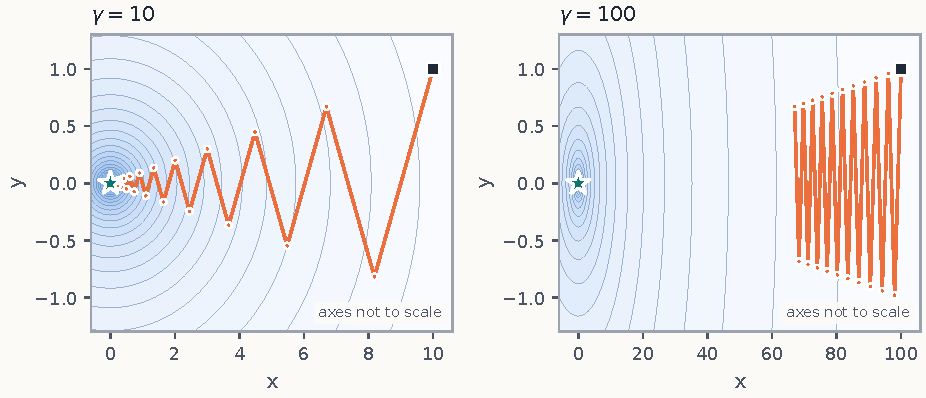
\includegraphics[width=0.6\textwidth]{fig_zigzag}\hfill
  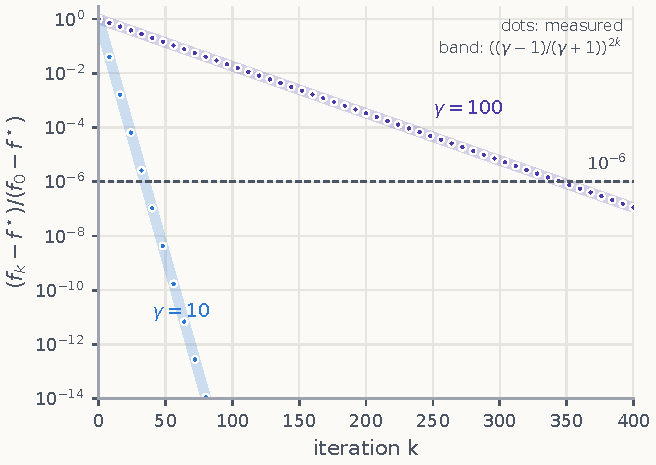
\includegraphics[width=0.37\textwidth]{fig_error_curves}

  \vspace{4pt}
  \raggedright
  \begin{itemize}\small
    \item On $f = \tfrac12(x^2+\gamma y^2)$ from $(\gamma,1)$, cutting $f$ by $10^6$ takes \textbf{35} steps when $\gamma = 10$
          and \textbf{346} when $\gamma=100$. That is about $3.45\,\kappa$.
    \item A perfect \emph{step length} cannot rescue a bad \emph{direction}. There are two ways out:
          change the geometry (preconditioning, next slide) or remember where you have been (momentum, Section~11).
  \end{itemize}
\end{frame}

\begin{frame}{The fix: change the geometry (preconditioning)}
  \begin{columns}[T]
    \begin{column}{0.48\textwidth}
      \small
      Run GD on $\tilde f(\y) = f(\bP^{-1/2}\y)$. In the original variables that is
      \[
        \x_{k+1} = \x_k - \alpha\,\bP^{-1}\nabla f(\x_k),
      \]
      with Hessian $\bP^{-1/2}\bA\bP^{-1/2}$. Pick $\bP\approx\bA$ and $\tilde\kappa\approx1$.
      \begin{itemize}\footnotesize
        \item \textbf{Centring features} (A1): $\kappa$ from $46.1$ to $1.5$, iterations from $319$ to $9$.
        \item \textbf{Jacobi scaling} $\bP = \diag(\bA)$ (A2): $\kappa$ from $1002$ to $1.065$.
        \item $\bP = \nabla^2 f$ is ideal but costly: Newton's method, left aside here.
      \end{itemize}
    \end{column}
    \begin{column}{0.5\textwidth}
      \centering
      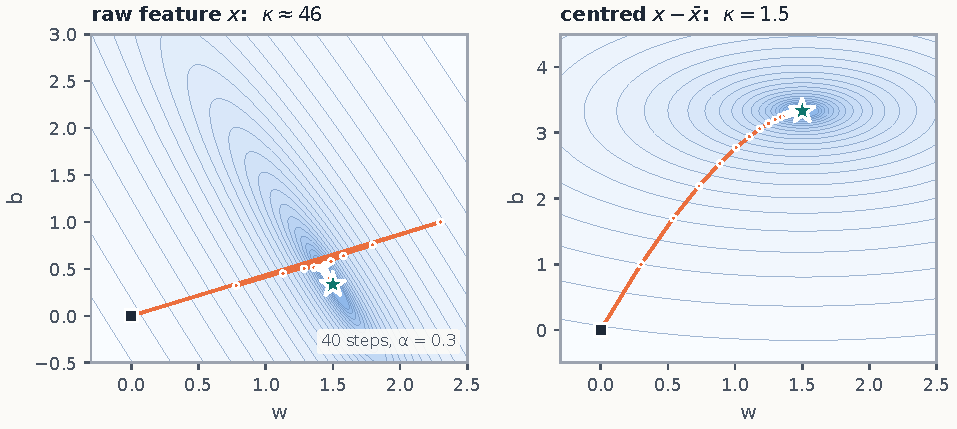
\includegraphics[width=\linewidth]{fig_scaling}

      \footnotesize The A1 regression before and after centring. The valley turns into a bowl.
    \end{column}
  \end{columns}
\end{frame}

\statement{WHY IT IS SLOW}{The step length is not the problem.\\ The direction is.}{Fix the geometry (preconditioning) or remember the past (momentum).}

% =====================================================================
%  9. Failure modes and pathological cases
% =====================================================================
\section{When gradient descent goes wrong}

\begin{frame}{Blow-ups, and functions with no global $L$}
  \begin{columns}[T]
    \begin{column}{0.5\textwidth}
      \textbf{1. Step too large} ($\alpha>2/L$): oscillating blow-up along the top eigenvector (M3(f), A3(d)).

      \vspace{4pt}
      \textbf{2. No global $L$.} For $f(x) = x^4$, $f'' = 12x^2$ keeps growing. With $\alpha = 0.1$,
      \[
        x_{k+1} = x_k\,(1 - 0.4x_k^2),
      \]
      which diverges exactly when $|x_0|>\sqrt5\approx2.236$:

      \vspace{2pt}
      \footnotesize
      \begin{tabular}{@{}l l@{}}
        $x_0 = 2.2$: & $-2.059,\ 1.434,\ 0.255,\ 0.249,\dots\to0$\\
        $x_0 = 2.3$: & $-2.567,\ 4.198,\ -25.39,\ 6521,\dots$
      \end{tabular}
    \end{column}
    \begin{column}{0.48\textwidth}
      \textbf{3. A flat minimum.} At $x^\star = 0$ we have $f''(0) = 0$, so $f$ is not strongly convex and the rate
      drops to \emph{sublinear}:
      \[
        x_{k+1}\approx x_k - 0.4x_k^3 \;\Rightarrow\; x_k\approx\frac{1}{\sqrt{0.8\,k}} .
      \]
      \footnotesize Check: at $k = 10^4$ the iteration gives $0.011176$ and the formula $0.011180$.

      \vspace{4pt}
      \begin{warnbox}[Lesson]
        \small A safe step depends on \emph{where you are}. A fixed $\alpha$ is only safe with a global $L$;
        otherwise let a line search pick the step (Section~10).
      \end{warnbox}
    \end{column}
  \end{columns}
\end{frame}

\begin{frame}{Saddle points: a trap with a trapdoor}
  \begin{columns}[T]
    \begin{column}{0.5\textwidth}
      \small
      $f = x^4+y^4-4xy$ has a saddle at $\mathbf 0$, with Hessian eigenvalues $-4$ along $(1,1)$ and $+4$ along $(1,-1)$.
      \begin{itemize}\footnotesize
        \item On the \textbf{stable manifold} $y=-x$, GD slides \emph{into the saddle} (M1).
        \item Elsewhere the unstable part grows by $1+4\alpha$ per step: escaping from distance $\delta = 10^{-3}$ takes
              about 21 steps ($\alpha = 0.1$).
      \end{itemize}
      \begin{thmbox}[Theorem \normalfont\cite{lee2016}]
        \footnotesize For $C^2$ $f$ with $L$-Lipschitz gradient and $\alpha<1/L$, GD from a random start
        converges to a strict saddle with probability zero.
      \end{thmbox}
    \end{column}
    \begin{column}{0.48\textwidth}
      \centering
      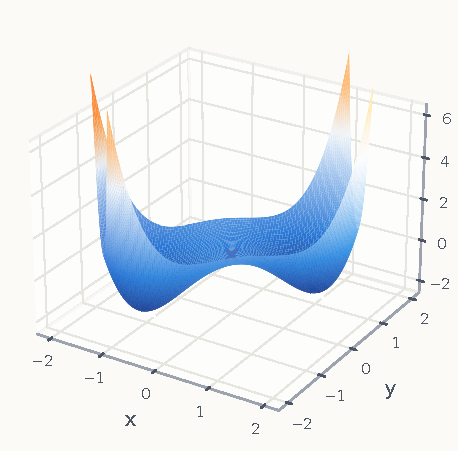
\includegraphics[width=0.7\linewidth]{fig_landscape_surface}

      \footnotesize\textcolor{mGrey}{GD almost never \emph{ends} at a saddle, but can idle near one: $\norm{\nabla f}$ is tiny there.}
    \end{column}
  \end{columns}
\end{frame}

\begin{frame}{Local minima: the starting point decides the answer}
  \begin{columns}[T]
    \begin{column}{0.52\textwidth}
      \centering
      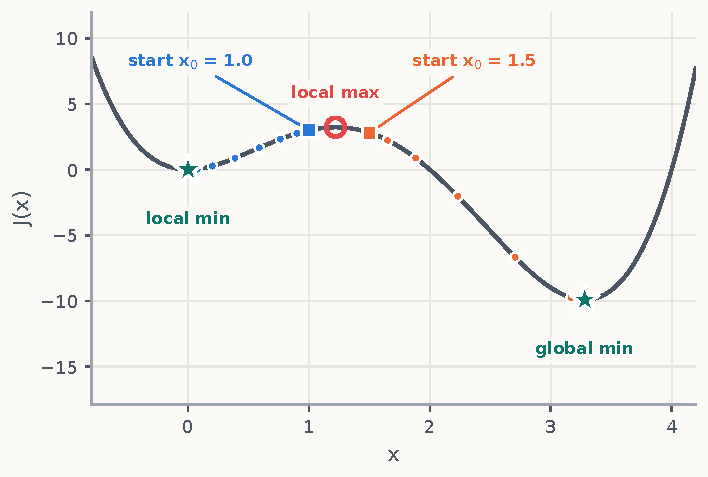
\includegraphics[width=\linewidth, height=0.6\textheight, keepaspectratio]{fig_local_minima}
    \end{column}
    \begin{column}{0.46\textwidth}
      \small
      $f(x) = x^4 - 6x^3 + 8x^2$ has two valleys with a hill at $x\approx1.22$.
      \begin{itemize}\footnotesize
        \item From $x_0 = 1.0$ GD rolls left into the \emph{local} minimum $x = 0$.
        \item From $x_0 = 1.5$ it rolls right into the \emph{global} minimum $x\approx3.28$.
      \end{itemize}
      GD may find \emph{a} minimum and miss \emph{the} best one.
      \begin{warnbox}[In practice]
        \footnotesize Try several starts and keep the best. The SSR of a line is convex: one minimum only.
      \end{warnbox}
    \end{column}
  \end{columns}
\end{frame}

\begin{frame}{Plateaus and curved valleys}
  \begin{columns}[T]
    \begin{column}{0.4\textwidth}
      \small
      \textbf{Plateau} (A4). For large $k$ the model $e^{-kt}$ is already close to zero, so it barely reacts to $k$
      and $J'\approx 10^{-3}$. A thousand steps from $k_0 = 6$ only reach $k\approx4.65$: a \alert{vanishing gradient}.

      \vspace{4pt}
      \textbf{The banana valley} (Rosenbrock)
      \[
        f = (1-x)^2+100\,(y-x^2)^2
      \]
      has $\kappa\approx2508$ at the minimum, and the valley \emph{bends}, so no single fixed rescaling straightens it.
      On the right: GD with Armijo against momentum over 2000 iterations.
    \end{column}
    \begin{column}{0.58\textwidth}
      \centering
      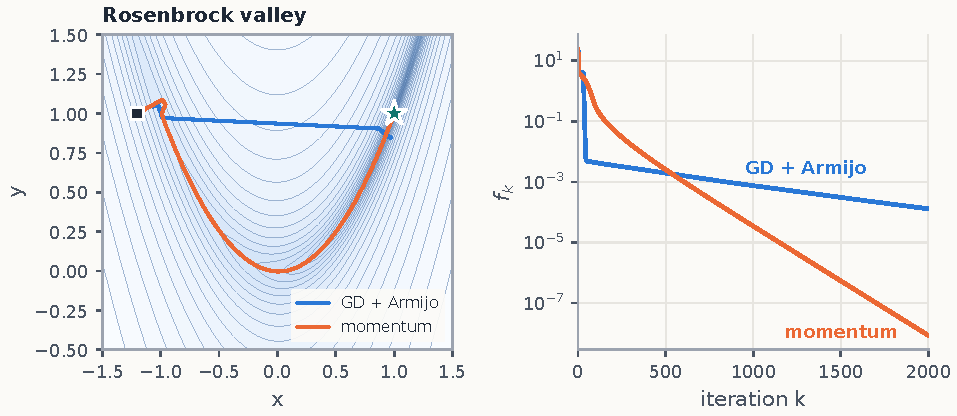
\includegraphics[width=\linewidth]{fig_rosenbrock}

      \footnotesize\textcolor{mGrey}{The A4 plateau itself is plotted in Problem A4 (solution 3 of 4).}
    \end{column}
  \end{columns}
\end{frame}

\begin{frame}{Nonsmooth objectives: a constant step never settles}
  $f(x) = |x|$ has ``gradient'' $\operatorname{sign}(x)$, whose size never shrinks near the minimum:
  $\;x_{k+1} = x_k - \alpha\operatorname{sign}(x_k)$.
  \vspace{4pt}
  \begin{itemize}\small
    \item The iterates march into the band $|x|\le\alpha$, then \alert{bounce around in it forever}: the error stays about $\alpha$.
    \item In the smooth case $\nabla f\to\mathbf 0$ shrinks the steps for free (Section~4). Here it does not.
    \item Remedy: shrink the steps yourself (the subgradient method), at the slower rate $O(1/\sqrt k)$~\cite{nesterov2018,boyd2004}.
  \end{itemize}
  \begin{keybox}[Where you meet this]
    \small $\ell_1$ regularisation, hinge loss, ReLU networks, max-type objectives. Smoothness is what makes a constant step work.
  \end{keybox}
\end{frame}

\begin{frame}{Finite precision: gradients by finite differences}
  \begin{columns}[T]
    \begin{column}{0.5\textwidth}
      \small
      No gradient formula? Try $\;f'(x)\approx\frac{f(x+h)-f(x)}{h}$, with error
      \[
        E(h)\approx\underbrace{\tfrac h2|f''|}_{\text{truncation}}+\underbrace{\tfrac{2\epsilon_{\text{mach}}|f|}{h}}_{\text{round-off}},
      \]
      smallest at $h^\star\sim\sqrt{\epsilon_{\text{mach}}}\approx1.5\times10^{-8}$. Going smaller makes it \emph{worse}.
      \begin{itemize}\footnotesize
        \item Forward: about 8 digits at best. Central: $h^\star\sim\epsilon^{1/3}$, error $\sim\epsilon^{2/3}\approx4\times10^{-11}$.
        \item Cost: $n$ extra $f$-evaluations per gradient (autodiff: a constant factor, Section~13).
        \item $\norm{\nabla f}$ has a noise floor: use relative stopping tests.
      \end{itemize}
    \end{column}
    \begin{column}{0.48\textwidth}
      \centering
      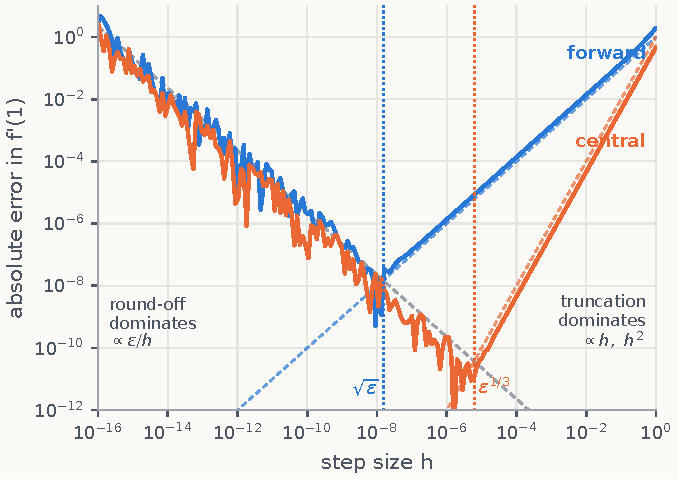
\includegraphics[width=\linewidth]{fig_fd_error}

      \footnotesize The classic V: truncation error on the right, round-off on the left ($f = e^x$ at $x = 1$).
    \end{column}
  \end{columns}
\end{frame}

% =====================================================================
%  10. Line search and adaptive step sizes
% =====================================================================
\section{Letting the method choose its own step}

\begin{frame}{Armijo backtracking: you do not need to know $L$}
  \begin{columns}[T]
    \begin{column}{0.5\textwidth}
      Accept a step only if it buys a fair share of the decrease the gradient promises.
      That is the \textbf{Armijo condition}, with $c\in(0,1)$:
      \[
        f(\x_k-\alpha\g_k)\le f(\x_k)-c\,\alpha\norm{\g_k}^2 .
      \]
      \begin{thmbox}[Backtracking \normalfont\cite{armijo1966}]
        \small
        $\alpha\gets\alpha_0$\\
        \textbf{while} Armijo fails: $\alpha\gets\beta\alpha$ \quad ($0<\beta<1$)\\
        $\x_{k+1}\gets\x_k-\alpha\g_k$
      \end{thmbox}
      \footnotesize Common choices: $c = 10^{-4}$, $\beta = \frac12$, and $\alpha_0 = 1$ or the previous step.
    \end{column}
    \begin{column}{0.48\textwidth}
      \begin{thmbox}[Theorem: backtracking always stops]
        \small If $\nabla f$ is $L$-Lipschitz, Armijo holds for every $\alpha\le\frac{2(1-c)}{L}$, so the step you accept satisfies
        \[ \alpha\ge\min\Bigl\{\alpha_0,\ \frac{2\beta(1-c)}{L}\Bigr\}. \]
      \end{thmbox}
      \small\textbf{Proof.}
      \pause
      The descent lemma gives $f(\x-\alpha\g)\le f(\x)-\alpha(1-\frac{\alpha L}{2})\norm{\g}^2$, and
      $1-\frac{\alpha L}2\ge c\iff\alpha\le\frac{2(1-c)}{L}$.
      \pause
      Backtracking stops at the first $\alpha_0\beta^j$ below that threshold, so it is never smaller than $\beta\cdot\frac{2(1-c)}{L}$. $\blacksquare$
    \end{column}
  \end{columns}
\end{frame}

\begin{frame}{What backtracking buys you}
  \begin{itemize}\small
    \item Every accepted step lowers $f$ by at least $c\,\alpha_{\min}\norm{\g_k}^2$, so \alert{all the rates from Section~7 survive},
          up to constants, without ever computing $L$~\cite{nocedal2006}.
    \item The step \emph{adapts to the local curvature}. It shrinks where the curvature is high, which cures the $x^4$ blow-up from Section~9,
          and with a generous first trial $\alpha_0$ it stays long where $f$ is flat.
    \item The price is a few extra evaluations of $f$ per iteration. No extra gradients are needed.
  \end{itemize}
  \vspace{2pt}
  \begin{keybox}[The Wolfe conditions]
    \small Add a curvature test, $\nabla f(\x_{k+1})\T\vd_k\ge c_2\nabla f(\x_k)\T\vd_k$ with $c<c_2<1$, and you also
    rule out steps that are too short. This pair is the standard line search in quasi-Newton software~\cite{nocedal2006}.
  \end{keybox}
\end{frame}

\begin{frame}{Barzilai--Borwein: a step size learned from the last move}
  \begin{columns}[T]
    \begin{column}{0.5\textwidth}
      \small
      With $\mathbf s_k = \x_k-\x_{k-1}$ and $\y_k = \g_k-\g_{k-1}$, pick the scalar $\beta = \tfrac1\alpha$ that best imitates
      the Hessian, $\beta\mathbf s_k\approx\y_k$:
      \[
        \min_{\beta}\norm{\beta\mathbf s_k-\y_k}^2 \;\Rightarrow\;
        \ans{\alpha_k^{\text{BB}} = \frac{\mathbf s_k\T\mathbf s_k}{\mathbf s_k\T\y_k}}
      \]
      \begin{itemize}\footnotesize
        \item On a quadratic, $1/\alpha_k$ is a Rayleigh quotient of $\bA$, between $\lmin$ and $\lmax$.
        \item \alert{Nonmonotone}: $\alpha_k$ can exceed $2/\lmax$ and $f$ can briefly rise, yet it is often far faster~\cite{barzilai1988}.
        \item For general $f$, add a nonmonotone line-search safeguard.
      \end{itemize}
    \end{column}
    \begin{column}{0.48\textwidth}
      \centering
      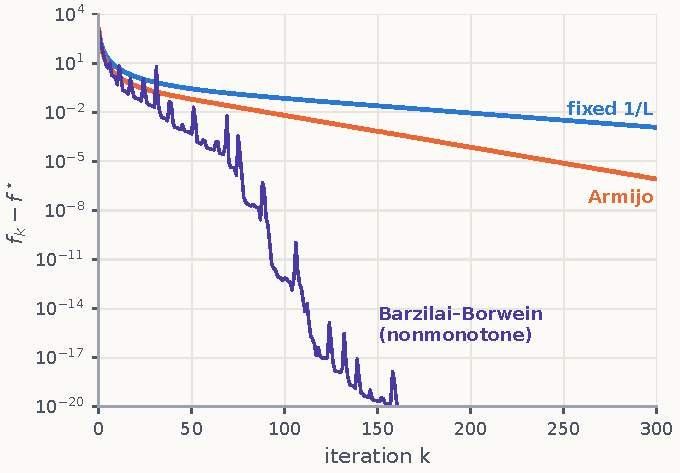
\includegraphics[width=\linewidth]{fig_linesearch}

      \footnotesize A diagonal quadratic with $n = 50$ and $\kappa = 100$. Fixed $1/L$ against Armijo against BB.
    \end{column}
  \end{columns}
\end{frame}

% =====================================================================
%  11. Momentum and Nesterov acceleration
% =====================================================================
\section{Momentum and acceleration}

\begin{frame}{Heavy-ball momentum: give the iterate some mass}
  \textbf{Polyak's heavy ball}~\cite{polyak1964}:
  $\quad\x_{k+1} = \x_k - \alpha\nabla f(\x_k) + \beta\,(\x_k-\x_{k-1}),\quad 0\le\beta<1.$

  \vspace{4pt}
  \small Where does that come from? Picture a ball of mass $m$ rolling on the landscape with friction $\gamma$:
  $\;m\ddot\x+\gamma\dot\x = -\nabla f(\x)$. Discretise with step $h$ (central difference for $\ddot\x$, forward for $\dot\x$):
  \[
    m\frac{\x_{k+1}-2\x_k+\x_{k-1}}{h^2}+\gamma\frac{\x_{k+1}-\x_k}{h} = -\nabla f(\x_k)
  \]
  \[
    \Longrightarrow\quad \x_{k+1} = \x_k - \underbrace{\tfrac{h^2}{m+\gamma h}}_{\alpha}\nabla f(\x_k) + \underbrace{\tfrac{m}{m+\gamma h}}_{\beta}(\x_k-\x_{k-1}).
  \]
  \begin{itemize}\small
    \item The velocity $\x_k-\x_{k-1}$ \alert{builds up} where the gradient keeps its sign (down the valley) and
          \alert{cancels} where it flips (across it), so the zig-zag is damped.
    \item Plain GD is the massless ball: $m\to0$, i.e.\ $\beta = 0$.
  \end{itemize}
\end{frame}

\begin{frame}{Why momentum is faster: look at the spectrum}
  \begin{columns}[T]
    \begin{column}{0.42\textwidth}
      \small Each eigen-direction obeys $r^2-(1+\beta-\alpha\lambda)r+\beta = 0$ (M5). Tuned well, every root sits on $|r| = \sqrt\beta$:
      \[
        \rho_{\text{HB}} = \tfrac{\sqrt\kappa-1}{\sqrt\kappa+1}
        \;\text{ vs. }\;
        \rho_{\text{GD}} = \tfrac{\kappa-1}{\kappa+1}.
      \]
      \begin{itemize}\footnotesize
        \item $\kappa = 100$: $0.818$ against $0.980$, so $69$ iterations instead of $691$.
        \item In general $O(\sqrt\kappa)$ instead of $O(\kappa)$.
        \item \alert{Caveat:} proven for quadratics only; counterexamples exist beyond~\cite{lessard2016}.
      \end{itemize}
    \end{column}
    \begin{column}{0.56\textwidth}
      \centering
      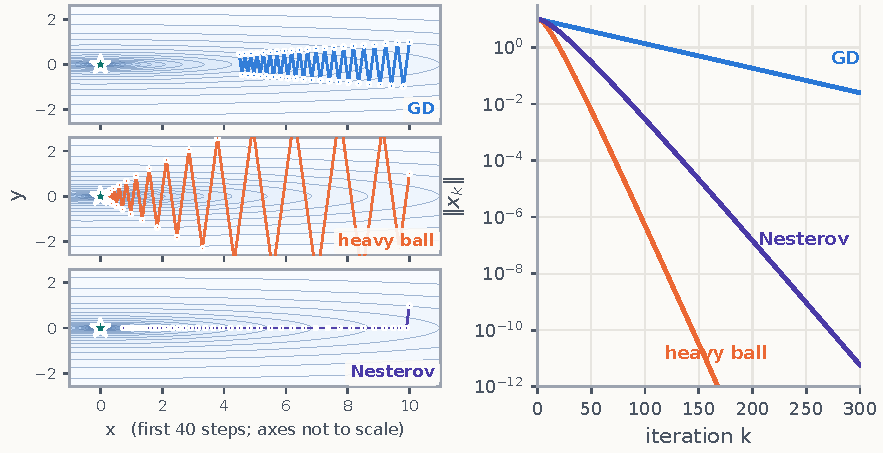
\includegraphics[width=\linewidth]{fig_momentum}

      \footnotesize $f = \frac12(x^2+100y^2)$: the first 40 steps of each method (left) and $\norm{\x_k}$ (right).
    \end{column}
  \end{columns}
\end{frame}

\begin{frame}{Nesterov's accelerated gradient}
  The trick is to \textbf{take the gradient at a look-ahead point}~\cite{nesterov1983}:
  \vspace{-4pt}
  \[
    \y_k = \x_k+\beta_k(\x_k-\x_{k-1}),\qquad \x_{k+1} = \y_k-\tfrac1L\nabla f(\y_k).
  \]
  \begin{thmbox}[Convex, $L$-smooth, $\beta_k = \frac{k-1}{k+2}$]
    \vspace{-4pt}
    \[ f(\x_k)-f^\star\le\frac{2L\norm{\x_0-\x^\star}^2}{(k+1)^2}\qquad\text{vs. GD: } \frac{L\norm{\x_0-\x^\star}^2}{2k}. \]
  \end{thmbox}
  \begin{thmbox}[$\mu$-strongly convex, $\beta = \frac{\sqrt\kappa-1}{\sqrt\kappa+1}$]
    \vspace{-4pt}
    \[ f(\x_k)-f^\star\le\Bigl(1-\tfrac1{\sqrt\kappa}\Bigr)^k\Bigl(f(\x_0)-f^\star+\tfrac\mu2\norm{\x_0-\x^\star}^2\Bigr). \]
  \end{thmbox}
  \footnotesize GD's bound after $10^4$ steps, Nesterov reaches after about $200$, for \emph{every} smooth convex function~\cite{nesterov2018}.
  Continuous-time limit: $\ddot\x+\frac3t\dot\x+\nabla f = 0$~\cite{su2016}, a heavy ball with fading friction.
\end{frame}

\begin{frame}{Optimality: no first-order method can do better}
  \begin{thmbox}[Lower bounds \normalfont\cite{nesterov2018}]
    \small For any method with iterates in $\x_0+\operatorname{span}\{\nabla f(\x_0),\dots,\nabla f(\x_{k-1})\}$
    (Nesterov matches both up to a constant):
    \begin{itemize}
      \item convex, $L$-smooth (high enough dimension): $f(\x_k)-f^\star\ge\frac{3L\norm{\x_0-\x^\star}^2}{32(k+1)^2}$;
      \item strongly convex: $\norm{\x_k-\x^\star}\ge\bigl(\frac{\sqrt\kappa-1}{\sqrt\kappa+1}\bigr)^k\norm{\x_0-\x^\star}$.
    \end{itemize}
  \end{thmbox}
  \centering\footnotesize
  \begin{tabular}{@{}l c c c@{}}
    \toprule
    & GD & Heavy ball & Nesterov \\
    \midrule
    convex rate & $O(1/k)$ & no guarantee & $O(1/k^2)$ \textcolor{mGreen}{(optimal)} \\
    strongly convex & $O(\kappa\log\frac1\varepsilon)$ & $O(\sqrt\kappa\log\frac1\varepsilon)$ on quadratics & $O(\sqrt\kappa\log\frac1\varepsilon)$ \textcolor{mGreen}{(optimal)} \\
    $f(\x_k)$ always decreases? & yes ($\alpha\le\frac1L$) & no & no (``ripples'') \\
    \bottomrule
  \end{tabular}
\end{frame}

\statement{THE PRICE OF A PROBLEM}{The condition number $\kappa$\\ decides how many steps you pay.}{GD pays $O(\kappa)$. Nesterov pays $O(\sqrt\kappa)$, and nothing that only sees gradients can do better.}

\begin{frame}{Acceleration in practice}
  \begin{columns}[T]
    \begin{column}{0.54\textwidth}
      \centering
      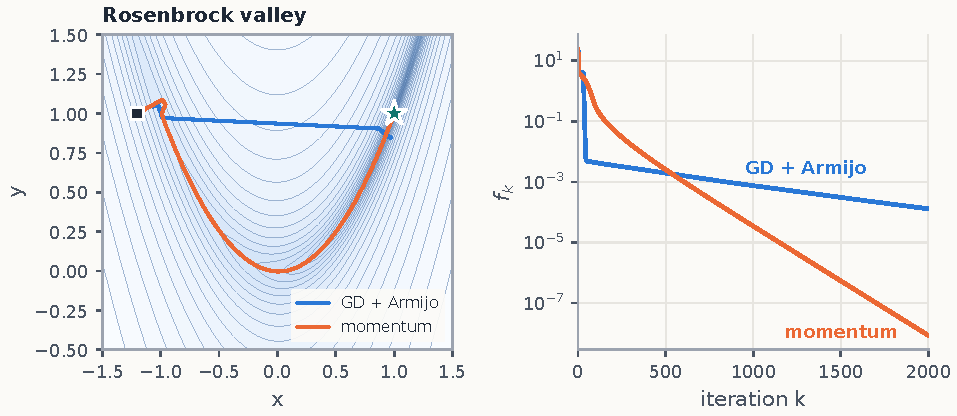
\includegraphics[width=\linewidth]{fig_rosenbrock}
    \end{column}
    \begin{column}{0.44\textwidth}
      \footnotesize
      \begin{itemize}
        \item On Rosenbrock, after 2000 iterations, momentum ($\beta = 0.9$) is down to $f\approx10^{-8}$ while
              GD with Armijo is stuck near $10^{-4}$.
        \item Momentum methods are \alert{non-monotone}. $f$ ripples up and down as the ball overshoots and swings back.
        \item A common practical fix: \emph{restart} the momentum whenever $f$ goes up.
        \item Momentum is built into the optimisers people actually use, such as SGD with momentum and Adam (Section~13).
      \end{itemize}
      \footnotesize\textcolor{mGrey}{For more intuition, see \cite{goh2017}.}
    \end{column}
  \end{columns}
\end{frame}

% =====================================================================
%  12. Stochastic gradient descent
% =====================================================================
\section{Stochastic gradient descent}

\begin{frame}{When even one gradient is too expensive}
  A training loss averages over $N$ data points:
  \[
    f(\x) = \frac1N\sum_{i=1}^N f_i(\x), \qquad \text{so one } \nabla f \text{ costs } N \text{ component gradients.}
  \]
  \textbf{SGD} cheats: pick one $i_k$ at random and step $\;\x_{k+1} = \x_k-\alpha_k\nabla f_{i_k}(\x_k)$.
  \begin{itemize}\small
    \item It is \textbf{unbiased}: $\E_{i}[\nabla f_i(\x)] = \nabla f(\x)$, so SGD is gradient descent \emph{on average}.
    \item A step costs the same whatever $N$ is. With $N = 10^6$, one GD step buys a million SGD steps.
    \item A \textbf{mini-batch} of $B$ samples cuts the gradient variance to $\sigma^2/B$, at $B$ times the cost.
  \end{itemize}
  \begin{keybox}[The catch]
    \small The noise does \emph{not} switch off at the answer: $\nabla f(\x^\star) = \mathbf 0$, but $\nabla f_i(\x^\star)\ne\mathbf 0$.
    With a constant step, SGD keeps jittering and never settles exactly.
  \end{keybox}
\end{frame}

\begin{frame}{Batch, stochastic and mini-batch on the line fit}
  \centering
  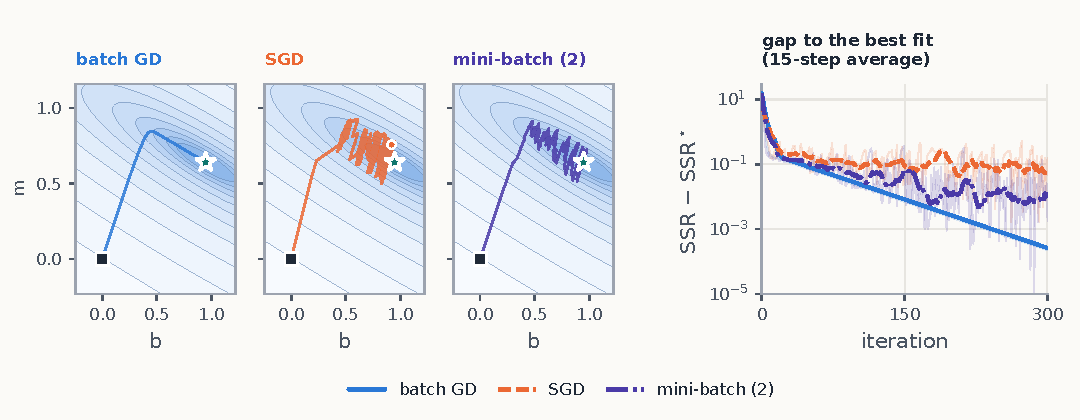
\includegraphics[width=\textwidth, height=0.55\textheight, keepaspectratio]{fig_sgd_paths}

  \raggedright\small
  \begin{itemize}
    \item One-point gradients are \emph{unbiased}: on average they equal the full gradient.
    \item Their noise does not vanish at the minimum, so with a fixed $\alpha$ SGD keeps jittering.
          Averaging $B$ points cuts the variance by $B$; a decaying $\alpha$ lets the path settle.
  \end{itemize}
\end{frame}

\begin{frame}{The noise ball, and how to shrink it}
  \begin{columns}[T]
    \begin{column}{0.46\textwidth}
      \small
      \textbf{Solvable case} (A5): $F = \frac12\E(x-\xi)^2$, constant $\alpha$:
      \[ \operatorname{Var}(x_k)\to\frac{\alpha\sigma^2}{2-\alpha}. \]
      \textbf{Any strongly convex $f$}~\cite{bottou2018}:
      \begin{itemize}\footnotesize
        \item fixed $\alpha$: linear drop, but only to a floor $\propto\alpha$;
        \item $\alpha_k = O(1/k)$: $\E[f(\x_k)-f^\star] = O(1/k)$ all the way.
      \end{itemize}
      \textbf{Robbins--Monro}~\cite{robbins1951}: $\sum_k\alpha_k = \infty$ (travel far enough) and
      $\sum_k\alpha_k^2<\infty$ (noise averages out).
    \end{column}
    \begin{column}{0.52\textwidth}
      \centering
      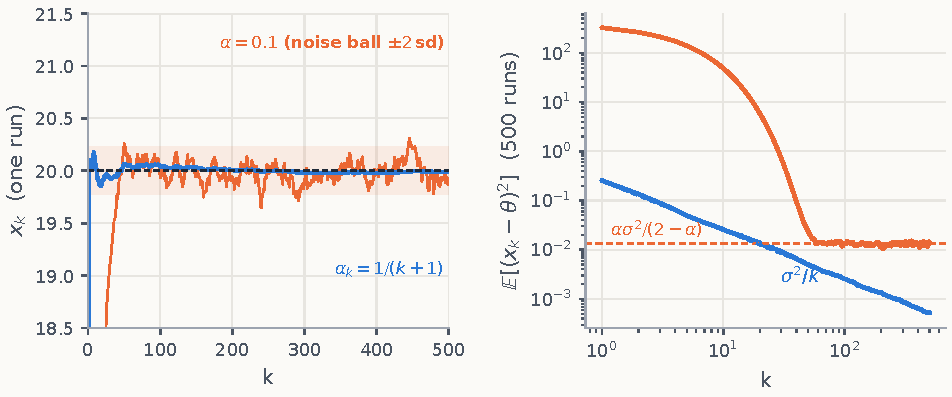
\includegraphics[width=\linewidth]{fig_sgd}

      \footnotesize With constant $\alpha = 0.1$ the error stalls at $\frac{\alpha\sigma^2}{2-\alpha}$; with $\alpha_k = \frac1{k+1}$
      it keeps falling like $\sigma^2/k$ (averaged over 500 runs).
    \end{column}
  \end{columns}
\end{frame}

\begin{frame}{SGD in practice}
  \begin{itemize}\small
    \item \textbf{Schedules.} Start with a large constant step for fast progress, then decay it to shrink the noise ball.
          Warm-up and step decay are the usual heuristics.
    \item \textbf{Epochs and shuffling.} Sweep through the data in a random order instead of sampling with replacement.
    \item \textbf{Batch size against step size.} A bigger $B$ gives a cleaner gradient but fewer steps for the same compute.
    \item \textbf{Total work} to reach accuracy $\varepsilon$ on a strongly convex problem, roughly:
  \end{itemize}
  \vspace{2pt}
  \centering\small
  \begin{tabular}{@{}l c c@{}}
    \toprule
    & Work per iteration & Iterations \\
    \midrule
    GD & $N$ & $O(\kappa\log\frac1\varepsilon)$ \\
    SGD & $1$ & $O(1/\varepsilon)$ (constants depend on $\kappa$ and the noise) \\
    \bottomrule
  \end{tabular}

  \vspace{4pt}
  \raggedright\footnotesize\textcolor{mGrey}{Huge $N$ and moderate accuracy (the usual ML situation): SGD's $N$-free step cost wins~\cite{bottou2018}.}
\end{frame}

% =====================================================================
%  13. Modern computational perspective
% =====================================================================
\section{Gradient methods today}

\begin{frame}{Why first-order methods won: gradients are cheap}
  \begin{thmbox}[Cheap gradient principle \normalfont\cite{griewank2008}]
    Reverse-mode automatic differentiation computes the \emph{whole} gradient $\nabla f\in\R^n$ for a small constant
    multiple of the cost of evaluating $f$ once, \alert{no matter how large $n$ is}.
  \end{thmbox}
  \vspace{2pt}
  \centering\small
  \begin{tabular}{@{}l c c@{}}
    \toprule
    How you get $\nabla f$ & Cost & Accuracy \\
    \midrule
    finite differences (Section~9) & $(n+1)\times$ cost$(f)$ & $\sim\sqrt{\epsilon_{\text{mach}}}$ \\
    forward-mode AD & $\sim n\times$ cost$(f)$ & machine precision \\
    reverse-mode AD (backpropagation) & $O(1)\times$ cost$(f)$ & machine precision \\
    \bottomrule
  \end{tabular}

  \raggedright
  \begin{itemize}\footnotesize
    \item Backpropagation in neural networks \emph{is} reverse-mode AD. That is why the gradient of a $10^9$-parameter
          model costs about as much as a few forward passes.
    \item GD itself only needs matrix--vector style operations, which run in parallel on GPUs.
  \end{itemize}
\end{frame}

\begin{frame}{Adam, and a puzzle called the edge of stability}
  \begin{columns}[T]
    \begin{column}{0.5\textwidth}
      \textbf{Adam}~\cite{kingma2015}, with all operations element-wise:
      \small
      \begin{align*}
        \mathbf m_k &= \beta_1\mathbf m_{k-1}+(1-\beta_1)\g_k \\
        \vv_k &= \beta_2\vv_{k-1}+(1-\beta_2)\g_k^{2}\\
        \x_{k+1} &= \x_k-\alpha\,\hat{\mathbf m}_k/\bigl(\sqrt{\hat\vv_k}+\epsilon\bigr)
      \end{align*}
      \small Read it as \alert{momentum} plus a \alert{diagonal preconditioner} $\bP_k = \diag(\sqrt{\hat\vv_k})$. In the language
      of Section~2, it is steepest descent in a diagonal norm that keeps changing. (The hats are a bias correction.)
    \end{column}
    \begin{column}{0.48\textwidth}
      \textbf{The edge of stability}~\cite{cohen2021}
      \begin{itemize}\small
        \item Classical theory says to keep $\alpha<2/L$.
        \item Yet in full-batch GD on neural networks, the \emph{sharpness} $\lmax(\nabla^2 f)$ is observed to climb until it
              reaches $2/\alpha$ and then hover just above it. The loss keeps going down over long horizons,
              though not monotonically.
        \item This is an \emph{empirical} finding that the classical analysis of Section~5 to Section~7 does not explain.
              It is an open research question.
      \end{itemize}
    \end{column}
  \end{columns}
\end{frame}

% =====================================================================
%  14. Summary / cheat sheet
% =====================================================================
\section{Summary}

\begin{frame}{The whole module on one slide}
  \centering\footnotesize
  \renewcommand{\arraystretch}{1.45}
  \begin{tabular}{@{}l l l l l@{}}
    \toprule
    Method & Step rule & Rate (str.\ convex) & Cost/iter. & Watch out for \\
    \midrule
    GD, fixed $\alpha$ & $\x-\alpha\nabla f$, $\alpha<2/L$ & $\frac{\kappa-1}{\kappa+1}$; $O(\kappa\log\frac1\varepsilon)$ & 1 grad & divergence, zig-zag \\
    GD + exact LS & $\argmin_\alpha f(\x-\alpha\g)$ & $(\frac{\kappa-1}{\kappa+1})^2$ in $f$ & 1 grad + 1-D & zig-zag \\
    GD + Armijo & backtracking & as GD, no $L$ needed & 1 grad + few $f$ & plateaus \\
    Barzilai--Borwein & $\mathbf s\T\mathbf s/\mathbf s\T\y$ & fast in practice & 1 grad & nonmonotone \\
    Heavy ball & $+\beta(\x_k-\x_{k-1})$ & $\frac{\sqrt\kappa-1}{\sqrt\kappa+1}$ (quadratics) & 1 grad & fails off quadratics \\
    Nesterov & grad.\ at look-ahead & $O(\sqrt\kappa\log\frac1\varepsilon)$ (optimal) & 1 grad & ripples \\
    SGD & $\x-\alpha_k\nabla f_{i_k}$ & $O(1/k)$, $\alpha_k\propto\frac1k$ & $\frac1N$ grad & noise ball \\
    \bottomrule
  \end{tabular}
\end{frame}

\begin{frame}{Five things to remember}
  \begin{enumerate}\small
    \item \textbf{Gradient descent is forward Euler on the gradient flow.} The step limit $\alpha<2/L$ is Euler's stability
          interval, and ill-conditioning is stiffness under another name.
    \item \textbf{The condition number $\kappa$ sets the price.} GD needs $O(\kappa)$ iterations; accelerated methods need
          $O(\sqrt\kappa)$, and no first-order method can do better.
    \item \textbf{One inequality powers the proofs.} The descent lemma, paired with convexity, strong convexity or PL,
          gives every rate in this module.
    \item \textbf{Failures are predictable.} Divergence, saddles, plateaus, nonsmoothness and round-off each leave a
          recognisable signature, and each has a known remedy.
    \item \textbf{Modern practice is the same idea at scale.} SGD, momentum, Adam and autodiff all build on the plain update
          $\x\gets\x-\alpha\nabla f$.
  \end{enumerate}
\end{frame}

\statement{IN ONE SENTENCE}{A gradient step is cheap.\\ The number of steps is the hard part.}{And the geometry of $f$ decides that number, which is what most of the numerical analysis is about.}


% ---------------- Part B: Problem set & solutions -------------------
% =====================================================================
%  Part B -- Problem set overview
% =====================================================================
\section{Part B: problems and complete solutions}

\begin{frame}{Ten problems, each solved step by step}
  \small
  Every problem is followed \alert{right away} by its full worked solution. Try each one yourself before
  you look at the next slide.

  \vspace{4pt}
  \begin{columns}[T]
    \begin{column}{0.49\textwidth}
      \textbf{Mathematical}
      \begin{itemize}\footnotesize
        \item[M1] Stationary points of a quartic landscape
        \item[M2] The descent lemma and the nonconvex rate
        \item[M3] Step-size stability on a coupled quadratic
        \item[M4] Exact line search and the zig-zag
        \item[M5] Heavy-ball momentum against plain GD
      \end{itemize}
    \end{column}
    \begin{column}{0.49\textwidth}
      \textbf{Real-life applications}
      \begin{itemize}\footnotesize
        \item[A1] Machine learning: regression and feature scaling
        \item[A2] Structural mechanics: a spring chain at rest
        \item[A3] Economics: two-product profit maximisation
        \item[A4] Parameter estimation: Newton's law of cooling
        \item[A5] Signal processing: calibrating a sensor with SGD
      \end{itemize}
    \end{column}
  \end{columns}

  \vspace{4pt}
  \footnotesize\textcolor{mGrey}{Difficulty: $\star$ routine \quad $\star\star$ several steps \quad $\star\star\star$ a proof or a deeper idea.
  Every number in the solutions was checked numerically.}
\end{frame}

% =====================================================================
%  M1 -- Stationary points of a quartic landscape
% =====================================================================
\subsection{M1: Stationary points of a quartic landscape}
\setprob{M1}

\begin{frame}{\probtitle{M1}{Stationary points of a quartic landscape}}
  \begin{probbox}[Problem M1 \hfill Mathematical \quad $\star\star$]
    Consider \(\displaystyle f(x,y) = x^4 + y^4 - 4xy\) on \(\R^2\).
    \begin{enumerate}[(a)]
      \item Compute $\nabla f$ and find \emph{all} stationary points.
      \item Classify each stationary point using the Hessian.
      \item Take one gradient-descent step from $\x_0=(1,0)$ with $\alpha = 0.1$,
            and check that $f$ goes down.
      \item Near the minimisers, which fixed step sizes keep GD locally stable?
            What happens if GD starts exactly at the saddle, or anywhere on the line $y=-x$?
    \end{enumerate}
  \end{probbox}
  \footnotesize\textcolor{mGrey}{What this practises: computing gradients, finding and classifying stationary points,
  and local step-size stability.}
\end{frame}

\begin{frame}{\soltitle{M1}{1}{4}}
  \textbf{(a) Gradient and stationary points.}
  \[
    \nabla f(x,y) = \begin{pmatrix} 4x^3 - 4y \\ 4y^3 - 4x \end{pmatrix} = \mathbf 0
    \quad\Longleftrightarrow\quad y = x^3, \;\; x = y^3 .
  \]
  Substitute the first equation into the second:
  \[
    x = (x^3)^3 = x^9 \;\Longrightarrow\; x\,(x^8 - 1) = 0 .
  \]
  Over $\R$, $x^8 = 1$ has only the roots $x = \pm 1$. So $x \in \{-1, 0, 1\}$, and with $y = x^3$ we get three points:
  \[
    \ans{(0,0),\quad (1,1),\quad (-1,-1)}
  \]
\end{frame}

\begin{frame}{\soltitle{M1}{2}{4}}
  \textbf{(b) Classify with the Hessian.}\quad
  $\displaystyle \nabla^2 f = \begin{pmatrix} 12x^2 & -4 \\ -4 & 12y^2 \end{pmatrix}.$
  \vspace{2pt}
  \begin{itemize}\small
    \item At $(0,0)$: $\begin{pmatrix} 0 & -4\\-4&0\end{pmatrix}$ has eigenvalues $-4$ (along $(1,1)$) and $+4$ (along $(1,-1)$).
          Indefinite, so this is a \alert{saddle point}, with $f=0$.
    \item At $(\pm1,\pm1)$: $\begin{pmatrix} 12 & -4\\-4&12\end{pmatrix}$ has eigenvalues $8$ (along $(1,1)$) and $16$ (along $(1,-1)$).
          Positive definite, so these are \alert{strict local minima}, with $f = 1+1-4 = -2$.
    \item Are they global? Since $4|xy| \le 2(x^2+y^2)$, we have $f \ge x^4+y^4-2(x^2+y^2) \to \infty$, so $f$ is coercive.
          Hence $f^\star = \ans{-2}$, reached at both minima.
  \end{itemize}
\end{frame}

\begin{frame}{\soltitle{M1}{3}{4}}
  \begin{columns}[T]
    \begin{column}{0.54\textwidth}
      \textbf{(c) One GD step from $\x_0 = (1,0)$ with $\alpha = 0.1$.}
      \[
        \g_0 = \nabla f(1,0) = (4-0,\; 0-4) = (4,-4)
      \]
      \[
        \x_1 = (1,0) - 0.1\,(4,-4) = \ans{(0.6,\;0.4)}
      \]
      \[
        f(\x_0) = 1, \qquad f(\x_1) = \ans{-0.8048}
      \]
      \footnotesize ($f(\x_1) = 0.6^4 + 0.4^4 - 4(0.24) = 0.1296 + 0.0256 - 0.96$.)
      \small We knew it would go down for small $\alpha$, because the
      directional derivative is $\nabla f\T(-\g_0) = -\norm{\g_0}^2 = -32 < 0$.
      Keep iterating with $\alpha = 0.1$ and you arrive at $(1,1)$.
    \end{column}
    \begin{column}{0.44\textwidth}
      \centering
      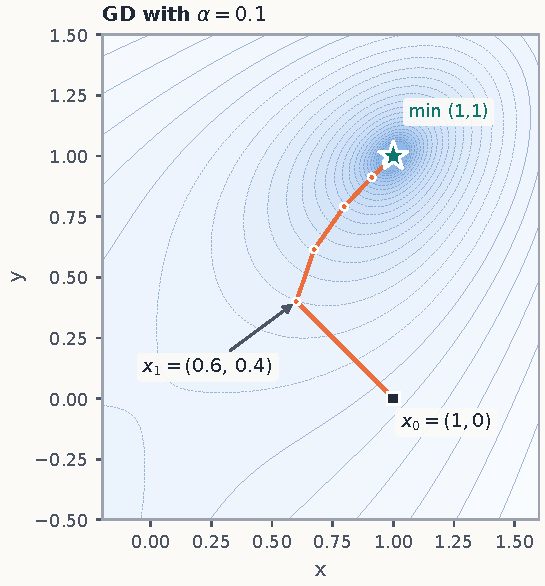
\includegraphics[width=0.95\linewidth]{fig_M1_step}
    \end{column}
  \end{columns}
\end{frame}

\begin{frame}{\soltitle{M1}{4}{4}}
  \textbf{(d) Local stability.} Near a minimiser, $\e_{k+1} \approx (\bI - \alpha\nabla^2 f(\x^\star))\,\e_k$,
  with eigen-factors $1 - 8\alpha$ and $1 - 16\alpha$. The stiffer one decides:
  \[
    |1-16\alpha| < 1 \;\Longleftrightarrow\; \ans{0 < \alpha < \tfrac{2}{16} = 0.125}
  \]
  The best local choice is $\alpha = \tfrac{2}{8+16} = \tfrac1{12}$, with local rate $\tfrac{16-8}{16+8} = \tfrac13$.
  \textbf{The saddle.} $\nabla f(0,0) = \mathbf 0$, so GD started there \alert{never moves at all}.
  On the line $y=-x$, $\nabla f(t,-t) = (4t^3+4t)(1,-1)$ keeps the iterates on the line, and $f(t,-t) = 2t^4+4t^2$
  is smallest at $t=0$. So GD \alert{slides into the saddle}: that line is its stable manifold.

  \begin{keybox}[Insight]
    Any nudge along $(1,1)$ grows by $1+4\alpha$ per step and escapes.
    Numerically, $(10^{-3},10^{-3})$ ends at $(1,1)$, while $(10^{-3},-10^{-3})$ ends at $(0,0)$.
    Saddles only capture a set of starting points of measure zero.
  \end{keybox}
\end{frame}

% =====================================================================
%  M2 -- Descent lemma and the nonconvex O(1/sqrt K) rate
% =====================================================================
\subsection{M2: Descent lemma and the nonconvex rate}
\setprob{M2}

\begin{frame}{\probtitle{M2}{The descent lemma and the nonconvex rate}}
  \begin{probbox}[Problem M2 \hfill Mathematical \quad $\star\star\star$]
    Let $f:\R^n\to\R$ be differentiable and bounded below by $f^\star$, with an
    $L$-Lipschitz gradient: $\norm{\nabla f(\x)-\nabla f(\y)} \le L\norm{\x-\y}$.
    \begin{enumerate}[(a)]
      \item Prove the \emph{descent lemma}:
            $f(\y) \le f(\x) + \nabla f(\x)\T(\y-\x) + \tfrac L2\norm{\y-\x}^2$.
      \item Show that GD, $\x_{k+1} = \x_k - \alpha\nabla f(\x_k)$, satisfies
            $f(\x_{k+1}) \le f(\x_k) - \alpha\bigl(1-\tfrac{\alpha L}{2}\bigr)\norm{\nabla f(\x_k)}^2$.
      \item Which $\alpha$ guarantee a decrease? Which $\alpha$ guarantees the largest one?
      \item Prove $\displaystyle\min_{0\le k<K}\norm{\nabla f(\x_k)} \le \sqrt{2L\,(f(\x_0)-f^\star)/K}$ for $\alpha = 1/L$.
      \item Use $f(x) = \tfrac L2 x^2$ to show that the bound in (b) cannot be improved.
    \end{enumerate}
  \end{probbox}
  \footnotesize\textcolor{mGrey}{What this practises: a careful proof, where the $2/L$ step window comes from,
  and convergence with no convexity at all.}
\end{frame}

\begin{frame}{\soltitle{M2}{1}{4}}
  \textbf{(a) The descent lemma.} Let $\vd = \y - \x$. By the fundamental theorem of calculus applied to
  $t\mapsto f(\x + t\vd)$,
  \[
    f(\y) - f(\x) = \int_0^1 \nabla f(\x + t\vd)\T\vd \,dt .
  \]
  Subtract $\nabla f(\x)\T\vd = \int_0^1 \nabla f(\x)\T\vd\,dt$ from both sides:
  \[
    f(\y) - f(\x) - \nabla f(\x)\T\vd
    = \int_0^1 \bigl[\nabla f(\x + t\vd) - \nabla f(\x)\bigr]\T\vd \,dt .
  \]
  Apply Cauchy--Schwarz, then the Lipschitz bound $\norm{\nabla f(\x+t\vd)-\nabla f(\x)} \le L\,t\norm{\vd}$:
  \[
    \le \int_0^1 L\,t\,\norm{\vd}^2\,dt = \frac L2\norm{\vd}^2 .
    \qquad\blacksquare
  \]
  \small\textcolor{mGrey}{In pictures: $f$ always stays below a parabola of curvature $L$ that touches it at $\x$.}
\end{frame}

\begin{frame}{\soltitle{M2}{2}{4}}
  \textbf{(b)} Put $\y = \x_{k+1} = \x_k - \alpha\g_k$ (so $\vd = -\alpha\g_k$) into (a):
  \[
    f(\x_{k+1}) \le f(\x_k) - \alpha\norm{\g_k}^2 + \frac{L\alpha^2}{2}\norm{\g_k}^2
    = f(\x_k) - \underbrace{\alpha\Bigl(1 - \frac{\alpha L}{2}\Bigr)}_{\varphi(\alpha)}\norm{\g_k}^2 .
  \]
  \textbf{(c)} $\varphi(\alpha) > 0 \iff \ans{0 < \alpha < 2/L}$. \quad
  $\varphi'(\alpha) = 1 - \alpha L = 0 \Rightarrow \ans{\alpha = 1/L}$, which gives $\varphi = \tfrac1{2L}$:
  \[
    f(\x_{k+1}) \le f(\x_k) - \frac{1}{2L}\norm{\nabla f(\x_k)}^2 .
  \]
  \begin{keybox}[What this means]
    The window $(0, 2/L)$ is \emph{exactly} the stability limit we found for quadratics ($\alpha < 2/\lmax$).
    The descent lemma carries it over to every $L$-smooth function.
  \end{keybox}
\end{frame}

\begin{frame}{\soltitle{M2}{3}{4}}
  \textbf{(d) Telescoping.} Add up the $\alpha = 1/L$ inequality for $k = 0,\dots,K-1$:
  \[
    \frac1{2L}\sum_{k=0}^{K-1}\norm{\g_k}^2 \le \sum_{k=0}^{K-1}\bigl(f(\x_k) - f(\x_{k+1})\bigr)
    = f(\x_0) - f(\x_K) \le f(\x_0) - f^\star .
  \]
  The smallest term is no bigger than the average, so
  \[
    K\min_{k<K}\norm{\g_k}^2 \le \sum_{k<K}\norm{\g_k}^2 \le 2L\bigl(f(\x_0)-f^\star\bigr)
    \;\Longrightarrow\;
    \ans{\min_{k<K}\norm{\g_k} \le \sqrt{\tfrac{2L(f(\x_0)-f^\star)}{K}}} \qquad\blacksquare
  \]
  \small
  \begin{itemize}
    \item The rate is $O(1/\sqrt K)$: reaching $\norm{\g}\le\varepsilon$ takes $K \ge 2L(f_0-f^\star)/\varepsilon^2$ iterations.
    \item We never used convexity. The price is that we only get \alert{a small gradient}, and the point we reach could be
          a saddle (compare M1).
  \end{itemize}
\end{frame}

\begin{frame}{\soltitle{M2}{4}{4}}
  \textbf{(e) The bound is tight.} Take $f(x) = \tfrac L2 x^2$, so $g = Lx$ and $x^+ = (1-\alpha L)x$.
  \[
    f(x) - f(x^+) = \frac L2 x^2\bigl[1 - (1-\alpha L)^2\bigr]
    = \frac L2 x^2\,(2\alpha L - \alpha^2L^2)
    = \alpha\Bigl(1 - \frac{\alpha L}{2}\Bigr)\underbrace{L^2x^2}_{g^2}.
  \]
  The inequality in (b) holds with \alert{equality}, so its constant cannot be improved in general.
  At $\alpha = 2/L$ we get $x^+ = -x$: the iterate bounces between $x$ and $-x$ forever and $f$ never drops.

  \vspace{4pt}
  \begin{keybox}[A numerical sanity check]
    For $f(\x) = \log(1+e^{\mathbf a\T\x}) + \tfrac12\norm{\x}^2$ with $L = \norm{\mathbf a}^2/4 + 1 = 2.25$,
    testing 20\,000 random pairs $(\x,\y)$ gives
    $\max\,[f(\y) - \text{bound}] = -5.6\times10^{-4} \le 0$. The lemma holds every time.
  \end{keybox}
\end{frame}

% =====================================================================
%  M3 -- Step-size stability on a coupled quadratic
% =====================================================================
\subsection{M3: Step-size stability on a coupled quadratic}
\setprob{M3}

\begin{frame}{\probtitle{M3}{Step-size stability on a coupled quadratic}}
  \begin{probbox}[Problem M3 \hfill Mathematical \quad $\star\star$]
    Let $f(\x) = \tfrac12\x\T\bA\x - \vb\T\x$ with
    $\bA = \begin{pmatrix}3&1\\1&3\end{pmatrix}$, $\vb = \begin{pmatrix}4\\4\end{pmatrix}$,
    and run GD, $\x_{k+1} = \x_k - \alpha\nabla f(\x_k)$.
    \begin{enumerate}[(a)]
      \item Find $\x^\star$ and show that $\e_k = \x_k - \x^\star$ obeys $\e_{k+1} = (\bI - \alpha\bA)\,\e_k$.
      \item Use the eigenpairs of $\bA$ to find \emph{all} $\alpha$ for which GD converges from every $\x_0$.
      \item Find the $\alpha$ that makes the worst-case contraction factor smallest, and that factor.
      \item With this $\alpha$ and $\x_0 = (3,0)$, compute $\x_1,\x_2$ and check that $\norm{\e_2} = \norm{\e_0}/9$.
      \item How many iterations guarantee $\norm{\e_k}\le 10^{-6}\norm{\e_0}$?
      \item Describe exactly what happens when $\alpha = 0.6$.
    \end{enumerate}
  \end{probbox}
  \footnotesize\textcolor{mGrey}{What this practises: an exact stability analysis, the best fixed step, and comparing step choices.}
\end{frame}

\begin{frame}{\soltitle{M3}{1}{4}}
  \textbf{(a)} Solve $\nabla f(\x) = \bA\x - \vb = \mathbf 0$. Since $\det\bA = 8$,
  \[
    \x^\star = \bA^{-1}\vb = \frac18\begin{pmatrix}3&-1\\-1&3\end{pmatrix}\begin{pmatrix}4\\4\end{pmatrix}
    = \ans{\begin{pmatrix}1\\1\end{pmatrix}} .
  \]
  Using $\vb = \bA\x^\star$:
  $\;\e_{k+1} = \x_k - \alpha(\bA\x_k - \bA\x^\star) - \x^\star = (\bI - \alpha\bA)\,\e_k .$

  \vspace{4pt}
  \textbf{Eigen-decomposition.} $\det(\bA-\lambda\bI) = (3-\lambda)^2 - 1 = 0$ gives
  \[
    \lambda_1 = 2,\;\; \vv_1 = \tfrac1{\sqrt2}(1,-1)\T; \qquad
    \lambda_2 = 4,\;\; \vv_2 = \tfrac1{\sqrt2}(1,1)\T .
  \]
  Writing $\e_k = c_1^{(k)}\vv_1 + c_2^{(k)}\vv_2$ splits the iteration into two separate scalar ones:
  \[
    c_i^{(k)} = (1 - \alpha\lambda_i)^k\, c_i^{(0)}, \qquad i = 1,2 .
  \]
\end{frame}

\begin{frame}{\soltitle{M3}{2}{4}}
  \begin{columns}[T]
    \begin{column}{0.5\textwidth}
      \textbf{(b)} To converge for \emph{every} $\e_0$ we need $|1-\alpha\lambda_i|<1$ for both $i$:
      \[
        0<\alpha<1 \;\text{ and }\; 0<\alpha<\tfrac12
      \]
      \[
        \Longrightarrow\;\ans{0 < \alpha < \tfrac{2}{\lmax} = \tfrac12}
      \]
      \textbf{(c)} $\rho(\alpha) = \max\{|1-2\alpha|,\,|1-4\alpha|\}$ is smallest where the two branches cross:
      \[
        1 - 2\alpha = -(1-4\alpha) \Rightarrow \ans{\alpha^\star = \tfrac13},\;\; \ans{\rho^\star = \tfrac13}
      \]
      \small In general $\alpha^\star = \frac{2}{\lmin+\lmax}$ and $\rho^\star = \frac{\kappa-1}{\kappa+1}$; here $\kappa = 2$.
    \end{column}
    \begin{column}{0.48\textwidth}
      \centering
      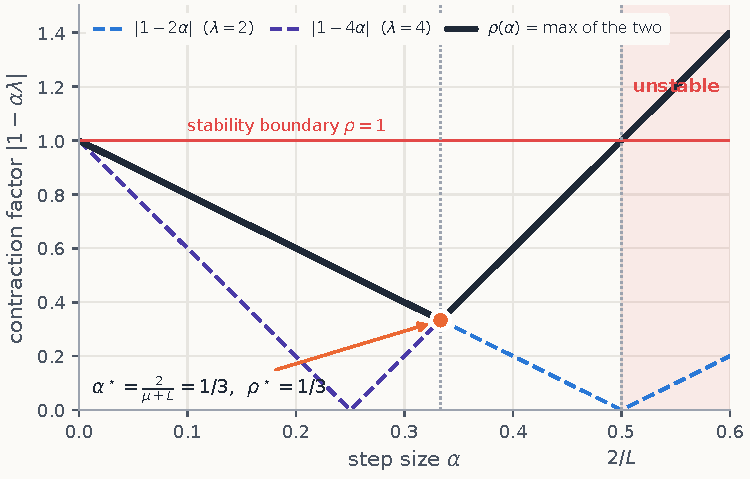
\includegraphics[width=\linewidth]{fig_amplification}
    \end{column}
  \end{columns}
\end{frame}

\begin{frame}{\soltitle{M3}{3}{4}}
  \textbf{(d)} With $\alpha = \tfrac13$ and $\x_0 = (3,0)$:
  \begin{align*}
    \g_0 &= \bA\x_0 - \vb = (9,3) - (4,4) = (5,-1), &
    \x_1 &= (3,0) - \tfrac13(5,-1) = \ans{\bigl(\tfrac43,\tfrac13\bigr)}\\
    \g_1 &= \bigl(4+\tfrac13,\ \tfrac43+1\bigr) - (4,4) = \bigl(\tfrac13,-\tfrac53\bigr), &
    \x_2 &= \bigl(\tfrac43-\tfrac19,\ \tfrac13+\tfrac59\bigr) = \ans{\bigl(\tfrac{11}9,\tfrac89\bigr)}
  \end{align*}
  So $\e_0 = (2,-1)$ and $\e_2 = \bigl(\tfrac29,-\tfrac19\bigr) = \tfrac19\,\e_0$, which gives $\norm{\e_2} = \norm{\e_0}/9$. \checkmark

  \vspace{4pt}
  \textbf{Why exactly $1/9$?} Split $\e_0 = \tfrac12(1,1) + \tfrac32(1,-1)$. The factors are
  $1-\tfrac43 = -\tfrac13$ on $(1,1)$ and $1-\tfrac23 = \tfrac13$ on $(1,-1)$. Both have size $\tfrac13$,
  so \emph{every} component shrinks by $\tfrac13$ per step: the optimal step \alert{balances} the two modes.
  \[
    \e_1 = -\tfrac16(1,1) + \tfrac12(1,-1) = \bigl(\tfrac13,-\tfrac23\bigr) \;\checkmark
  \]
\end{frame}

\begin{frame}{\soltitle{M3}{4}{4}}
  \textbf{(e)} $\norm{\e_k} = 3^{-k}\norm{\e_0}$, so we need $3^{-k} \le 10^{-6}$:
  \vspace{-4pt}
  \[
    k \ge \frac{6\ln 10}{\ln 3} = \frac{13.8155}{1.0986} = 12.58
    \;\Longrightarrow\; \ans{k = 13}
  \]
  \textbf{(f) $\alpha = 0.6 > 0.5$.} The factors are $1 - 0.6\cdot2 = -0.2$ and $1 - 0.6\cdot4 = \alert{-1.4}$:
  \[
    \e_k = \tfrac12(-1.4)^k(1,1) + \tfrac32(-0.2)^k(1,-1).
  \]
  \begin{itemize}\small
    \item The $(1,1)$ mode \alert{grows} $\times1.4$ per step, flipping sign each time: $\e_6 \approx (3.765, 3.765)$.
    \item The $(1,-1)$ mode still decays. One stiff direction ($\lmax$) sets the step limit.
  \end{itemize}
  \begin{keybox}[Lesson]
    The blow-up happens along the eigenvector of $\lmax$, just as it does for explicit Euler on a stiff ODE.
  \end{keybox}
\end{frame}

% =====================================================================
%  M4 -- Exact line search, orthogonal zig-zag, conditioning
% =====================================================================
\subsection{M4: Exact line search and the zig-zag}
\setprob{M4}

\begin{frame}{\probtitle{M4}{Exact line search, the zig-zag, and conditioning}}
  \begin{probbox}[Problem M4 \hfill Mathematical \quad $\star\star\star$]
    Steepest descent with \emph{exact line search}:
    $\x_{k+1} = \x_k - \alpha_k\g_k$, $\;\alpha_k = \argmin_{\alpha>0} f(\x_k - \alpha\g_k)$.
    \begin{enumerate}[(a)]
      \item For $f(\x) = \tfrac12\x\T\bA\x$ with $\bA \succ 0$, show that $\alpha_k = \dfrac{\g_k\T\g_k}{\g_k\T\bA\g_k}$.
      \item Prove that consecutive gradients are orthogonal: $\g_{k+1}\T\g_k = 0$.
      \item For $f(x,y) = \tfrac12(x^2 + \gamma y^2)$, $\gamma\ge1$, $\x_0 = (\gamma,1)$, prove by induction that
            $x_k = \gamma r^k$ and $y_k = (-r)^k$, with $r = \frac{\gamma-1}{\gamma+1}$.
      \item Deduce $f(\x_k) = r^{2k}f(\x_0)$ and compare it with the Kantorovich bound.
      \item How many iterations reduce $f$ by a factor $10^6$ when $\gamma = 10$, and when $\gamma = 100$?
    \end{enumerate}
  \end{probbox}
  \footnotesize\textcolor{mGrey}{What this practises: a derivation, a proof by induction, and how conditioning sets the rate.
  The closed form in (c) is a classical example (Boyd \& Vandenberghe~\cite{boyd2004}, Section~9.3.2).}
\end{frame}

\begin{frame}{\soltitle{M4}{1}{4}}
  \textbf{(a)} Let $\varphi(\alpha) = f(\x - \alpha\g) = \tfrac12(\x-\alpha\g)\T\bA(\x-\alpha\g)$, where $\g = \bA\x$.
  \[
    \varphi'(\alpha) = -\g\T\bA(\x - \alpha\g) = -\g\T\g + \alpha\,\g\T\bA\g = 0
    \;\Longrightarrow\; \ans{\alpha_k = \frac{\g_k\T\g_k}{\g_k\T\bA\g_k}}
  \]
  Since $\varphi''(\alpha) = \g\T\bA\g > 0$, this is a minimum.

  \vspace{4pt}
  \textbf{(b)} From $\g_{k+1} = \bA\x_{k+1} = \g_k - \alpha_k\bA\g_k$,
  \[
    \g_k\T\g_{k+1} = \g_k\T\g_k - \alpha_k\,\g_k\T\bA\g_k = 0 \qquad\blacksquare
  \]
  \begin{keybox}[This is true for any smooth $f$]
    Exact line search means $\varphi'(\alpha_k) = -\nabla f(\x_{k+1})\T\g_k = 0$.
    So each step is at a \alert{right angle} to the one before it, and that is where the zig-zag comes from.
  \end{keybox}
\end{frame}

\begin{frame}{\soltitle{M4}{2}{4}}
  \textbf{(c) Induction.} The base case $k = 0$ is $\x_0 = (\gamma, 1)$ \checkmark.
  Now assume $\x_k = (\gamma r^k, (-r)^k)$. Here $\bA = \diag(1,\gamma)$, so
  \[
    \g_k = \bigl(\gamma r^k,\ \gamma(-r)^k\bigr),\quad
    \g_k\T\g_k = 2\gamma^2 r^{2k},\quad
    \g_k\T\bA\g_k = \gamma^2 r^{2k}(1+\gamma).
  \]
  The step turns out to be \emph{the same every time}: $\alpha_k = \dfrac{2}{1+\gamma}$. Then
  \begin{align*}
    x_{k+1} &= \gamma r^k\Bigl(1 - \tfrac{2}{1+\gamma}\Bigr) = \gamma r^k\cdot\tfrac{\gamma-1}{\gamma+1} = \gamma r^{k+1},\\
    y_{k+1} &= (-r)^k\Bigl(1 - \tfrac{2\gamma}{1+\gamma}\Bigr) = (-r)^k\cdot\tfrac{1-\gamma}{1+\gamma} = (-r)^{k+1}.
    \qquad\blacksquare
  \end{align*}
  \small The $y$-coordinate changes sign at every step: that is the zig-zag. For $\gamma = 10$, $\x_1 = (8.18,\,-0.818)$.
\end{frame}

\begin{frame}{\soltitle{M4}{3}{4}}
  \textbf{(d)}
  $\displaystyle f(\x_k) = \tfrac12\bigl(\gamma^2 r^{2k} + \gamma r^{2k}\bigr) = r^{2k}\cdot\tfrac12(\gamma^2+\gamma) = \ans{r^{2k}f(\x_0)}$.

  \smallskip
  The Kantorovich bound for steepest descent with exact line search says
  $f_{k+1} - f^\star \le \bigl(\tfrac{\kappa-1}{\kappa+1}\bigr)^2 (f_k - f^\star)$, and here $\kappa = \gamma$.
  This example \alert{hits the bound exactly}, so the bound cannot be improved.

  \vspace{4pt}
  \textbf{(e)} $r^{2k}\le10^{-6} \iff k \ge \dfrac{3\ln10}{\ln\frac{\gamma+1}{\gamma-1}}$:
  \[
    \gamma = 10:\; k \ge \frac{6.9078}{0.20067} = 34.4 \Rightarrow \ans{35},
    \qquad
    \gamma = 100:\; k \ge \frac{6.9078}{0.020001} = 345.4 \Rightarrow \ans{346}.
  \]
  For large $\gamma$, $\ln\frac{\gamma+1}{\gamma-1}\approx\frac2\gamma$, so $k \approx 3.45\,\gamma$.
  \alert{The work grows in proportion to the condition number.}
\end{frame}

\begin{frame}{\soltitle{M4}{4}{4}}
  \centering
  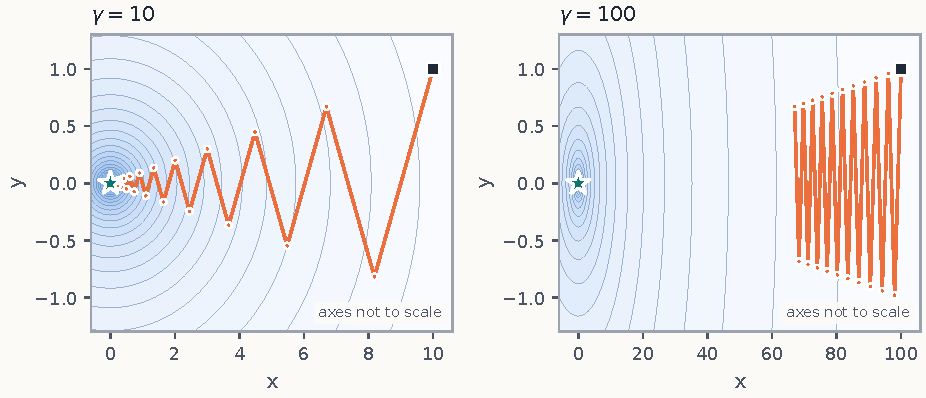
\includegraphics[width=0.56\textwidth]{fig_zigzag}\hfill
  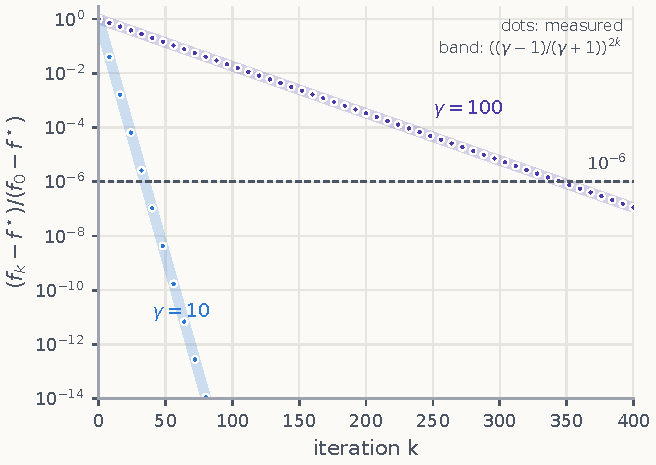
\includegraphics[width=0.34\textwidth]{fig_error_curves}

  \begin{keybox}[Takeaways]
    \small
    \begin{itemize}
      \item Even the \emph{best} step length along $-\g$ is slow: the \alert{direction} is the problem, which is why we need
            momentum (M5) and preconditioning (A1, A2).
      \item Start on an eigenvector, say $(1,0)$, and one step lands on the minimum. The worst case depends on $\x_0$.
    \end{itemize}
  \end{keybox}
\end{frame}

% =====================================================================
%  M5 -- Heavy-ball momentum vs plain GD: spectral comparison
% =====================================================================
\subsection{M5: Heavy-ball momentum vs.\ plain GD}
\setprob{M5}

\begin{frame}{\probtitle{M5}{Heavy-ball momentum against plain GD}}
  \begin{probbox}[Problem M5 \hfill Mathematical \quad $\star\star\star$]
    The heavy-ball (Polyak) iteration is
    $\x_{k+1} = \x_k - \alpha\nabla f(\x_k) + \beta(\x_k - \x_{k-1})$.
    Model each eigen-direction by $f(x) = \tfrac12\lambda x^2$ with $\lambda\in[\mu,L]$.
    \begin{enumerate}[(a)]
      \item Show that $x_{k+1} = (1+\beta-\alpha\lambda)x_k - \beta x_{k-1}$, and derive its characteristic polynomial.
      \item Show that when the roots are complex, $|r_1| = |r_2| = \sqrt\beta$, \emph{whatever $\lambda$ is}.
      \item For $\mu = 1$, $L = 100$, take
            $\alpha = \frac{4}{(\sqrt L+\sqrt\mu)^2}$ and $\beta = \bigl(\frac{\sqrt L-\sqrt\mu}{\sqrt L+\sqrt\mu}\bigr)^2$.
            Compute them, and show that every $\lambda\in[1,100]$ gives complex or repeated roots.
      \item How many iterations do GD (best $\alpha = \frac{2}{\mu+L}$) and heavy ball need to cut the error by $10^{6}$?
      \item What goes on at exactly $\lambda = \mu$?
    \end{enumerate}
  \end{probbox}
\end{frame}

\begin{frame}{\soltitle{M5}{1}{4}}
  \textbf{(a)} With $\nabla f = \lambda x$:
  $\;x_{k+1} = x_k - \alpha\lambda x_k + \beta x_k - \beta x_{k-1} = (1+\beta-\alpha\lambda)\,x_k - \beta\,x_{k-1}.$

  Trying $x_k = r^k$ gives the \textbf{characteristic polynomial}
  \[
    \ans{r^2 - (1+\beta-\alpha\lambda)\,r + \beta = 0},
    \qquad\text{with companion matrix } \mathbf T = \begin{pmatrix}1+\beta-\alpha\lambda & -\beta\\ 1 & 0\end{pmatrix}.
  \]
  The iteration converges iff the spectral radius $\rho(\mathbf T) = \max|r_i|$ is below 1.

  \vspace{4pt}
  \textbf{(b)} Vieta gives $r_1 r_2 = \beta$. If the roots are complex conjugates, $r_2 = \bar r_1$, so
  \[
    |r_1|^2 = r_1\bar r_1 = r_1 r_2 = \beta \;\Longrightarrow\; \ans{|r_{1,2}| = \sqrt\beta}.
  \]
  The roots are complex exactly when the discriminant is negative:
  \[
    (1+\beta-\alpha\lambda)^2 < 4\beta
    \iff (1-\sqrt\beta)^2 < \alpha\lambda < (1+\sqrt\beta)^2 .
  \]
\end{frame}

\begin{frame}{\soltitle{M5}{2}{4}}
  \textbf{(c)} Here $\kappa = L/\mu = 100$ and $\sqrt\kappa = 10$, so
  \[
    \alpha = \frac{4}{(10+1)^2} = \ans{\frac{4}{121}\approx 0.03306},
    \qquad
    \sqrt\beta = \frac{9}{11},\;\; \beta = \ans{\frac{81}{121}\approx 0.6694}.
  \]
  The edges of the complex region are
  \[
    (1-\sqrt\beta)^2 = \Bigl(\frac{2}{11}\Bigr)^2 = \frac{4}{121} = \alpha\mu,
    \qquad
    (1+\sqrt\beta)^2 = \Bigl(\frac{20}{11}\Bigr)^2 = \frac{400}{121} = \alpha L .
  \]
  So as $\lambda$ runs over $[1,100]$, $\alpha\lambda$ covers \emph{exactly} $[\tfrac4{121},\tfrac{400}{121}]$: complex roots inside,
  a double root at each end. Therefore
  \[
    \rho(\mathbf T) = \sqrt\beta = \frac{9}{11} \approx 0.818 \quad\text{for \emph{every} } \lambda\in[1,100].
  \]
  \small\textcolor{mGrey}{That is the whole point of this tuning: it puts the entire spectrum on the circle $|r| = \sqrt\beta$.}
\end{frame}

\begin{frame}{\soltitle{M5}{3}{4}}
  \begin{columns}[T]
    \begin{column}{0.53\textwidth}
      \textbf{(d)} Contraction factors, and iterations from $k \ge \ln 10^6 / \ln(1/\rho)$:
      \begin{align*}
        \rho_{\text{GD}} &= \tfrac{\kappa-1}{\kappa+1} = \tfrac{99}{101}, &
        k_{\text{GD}} &\ge \tfrac{13.8155}{0.0200} \Rightarrow \ans{691}\\[2pt]
        \rho_{\text{HB}} &= \tfrac{\sqrt\kappa-1}{\sqrt\kappa+1} = \tfrac{9}{11}, &
        k_{\text{HB}} &\ge \tfrac{13.8155}{0.2007} \Rightarrow \ans{69}
      \end{align*}
      That is about $10 = \sqrt\kappa$ times faster. In general the cost drops from
      $O(\kappa\log\tfrac1\varepsilon)$ to $O(\sqrt\kappa\log\tfrac1\varepsilon)$.
    \end{column}
    \begin{column}{0.44\textwidth}
      \centering
      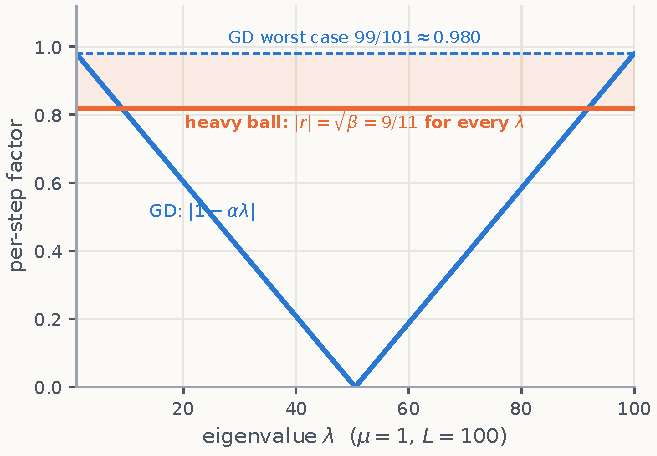
\includegraphics[width=\linewidth]{fig_hb_spectrum}
    \end{column}
  \end{columns}
\end{frame}

\begin{frame}{\soltitle{M5}{4}{4}}
  \textbf{(e) Repeated roots at the ends.} At $\lambda = \mu$ the discriminant is $0$ and there is a double root
  $r = \tfrac12(1+\beta-\alpha\mu) = \sqrt\beta = \tfrac9{11}$, so
  \[
    x_k = (c_1 + c_2\,k)\,r^k \qquad\text{(an extra factor of $k$ appears).}
  \]
  \begin{itemize}\small
    \item So the error is \emph{not} bounded by $1\cdot r^k$. From $x_0 = x_{-1} = 1$ with $\lambda = \mu$,
          heavy ball needs \alert{83} iterations for $|x_k|<10^{-6}$, not 69 (checked numerically); GD needs 691.
    \item Rates like $\rho_{\text{HB}}$ are \emph{asymptotic}: $\norm{\e_k}\le C(k)\,\rho^k$, where $C(k)$ grows at most polynomially.
  \end{itemize}
  \begin{warnbox}[Beyond quadratics, be careful]
    For a general strongly convex $f$, heavy ball with these parameters is not guaranteed to converge.
    Lessard, Recht and Packard give a counterexample~\cite{lessard2016}; Nesterov's method has a proof.
  \end{warnbox}
\end{frame}

% =====================================================================
%  A1 -- Machine learning: linear regression by GD, feature scaling
% =====================================================================
\subsection{A1: Machine learning, regression and feature scaling}
\setprob{A1}

\begin{frame}{\probtitle{A1}{Linear regression by GD, and why feature scaling matters}}
  \begin{probbox}[Problem A1 \hfill Application: Machine Learning \quad $\star\star$]
    A model $\hat y = wx + b$ is trained on the data $(1,2),\,(2,3),\,(3,5)$ by minimising the
    mean-squared-error loss
    \[
      \mathcal L(w,b) = \frac{1}{2n}\sum_{i=1}^{n}\bigl(wx_i + b - y_i\bigr)^2, \qquad n = 3 .
    \]
    \vspace{-8pt}
    \begin{enumerate}[(a)]
      \item Derive $\nabla\mathcal L$ and take two GD steps from $(0,0)$ with $\alpha = 0.1$.
      \item Find the Hessian, its eigenvalues, $\kappa$, and the largest stable $\alpha$.
      \item Replace $x$ by the centred feature $\tilde x = x - \bar x$. Recompute the Hessian and $\kappa$, and
            compare the iterations needed for $10^{-6}$ accuracy at the best fixed step.
      \item Find the optimal $(w,b)$ and explain what you see.
    \end{enumerate}
  \end{probbox}
  \footnotesize\textcolor{mGrey}{The point: training \emph{is} gradient descent, and preprocessing is preconditioning.}
\end{frame}

\begin{frame}{\soltitle{A1}{1}{4}}
  \textbf{(a) Gradient.} With residuals $r_i = wx_i + b - y_i$,
  \[
    \frac{\partial\mathcal L}{\partial w} = \frac1n\sum_i r_i x_i, \qquad
    \frac{\partial\mathcal L}{\partial b} = \frac1n\sum_i r_i .
  \]
  \textbf{Step 1} from $(0,0)$: $\;r = (-2,-3,-5)$ and $\;\mathcal L = 6.3333$.
  \[
    \nabla\mathcal L = \Bigl(\tfrac{-2-6-15}{3},\ \tfrac{-10}{3}\Bigr) = (-7.6667,\,-3.3333)
    \;\Rightarrow\; (w_1,b_1) = \ans{(0.7667,\ 0.3333)}
  \]
  and the loss drops to $\mathcal L(w_1,b_1) = 1.2826$.
  \textbf{Step 2}: the predictions are $(1.1000,\,1.8667,\,2.6333)$, so $r = (-0.9000,\,-1.1333,\,-2.3667)$.
  \[
    \nabla\mathcal L = \Bigl(\tfrac{-0.9-2.2667-7.1}{3},\ \tfrac{-4.4}{3}\Bigr) = (-3.4222,\,-1.4667)
  \]
  \[
    (w_2,b_2) = \ans{(1.1089,\ 0.4800)}, \qquad \mathcal L = 0.2807 .
  \]
\end{frame}

\begin{frame}{\soltitle{A1}{2}{4}}
  \textbf{(b) Hessian.} $\mathcal L$ is quadratic, so the Hessian is constant:
  $\;\bH = \frac1n\sum_i\begin{pmatrix}x_i^2 & x_i\\ x_i & 1\end{pmatrix}
        = \begin{pmatrix}14/3 & 2\\ 2 & 1\end{pmatrix}.$
  \smallskip
  $\lambda^2 - \tfrac{17}{3}\lambda + \tfrac23 = 0 \;\Rightarrow\; \lambda = \dfrac{17\pm\sqrt{265}}{6}$, so
  \[
    \lmax = 5.5465,\quad \lmin = 0.1202,\quad
    \ans{\kappa \approx 46.1},\quad \ans{\alpha < \tfrac{2}{\lmax} \approx 0.3606}
  \]
  The best fixed step is $\alpha^\star = \tfrac{2}{\lmin+\lmax} = \tfrac{6}{17} \approx 0.353$. Its rate is
  $\tfrac{\kappa-1}{\kappa+1} = 0.9576$, which means \alert{319 iterations} to reach $10^{-6}$. For three data points!

  \begin{keybox}[Why is such a tiny problem so badly conditioned?]
    Every $x_i$ is positive ($\bar x = 2$), so the columns $[\,x,\ \mathbf 1\,]$ are strongly correlated.
    Nudging $w$ or nudging $b$ changes the fit in almost the same way, and that makes a long, narrow valley.
  \end{keybox}
\end{frame}

\begin{frame}{\soltitle{A1}{3}{4}}
  \textbf{(c) Centring.} $\tilde x = x - 2 = (-1,0,1)$, so $\overline{\tilde x} = 0$ and $\overline{\tilde x^2} = \tfrac23$:
  \[
    \tilde\bH = \begin{pmatrix}2/3 & 0\\ 0 & 1\end{pmatrix}
    \;\Rightarrow\; \ans{\kappa = 1.5},\quad
    \alpha^\star = \frac{2}{2/3+1} = 1.2,\quad \rho = \frac{0.5}{2.5} = 0.2 .
  \]
  Iterations for $10^{-6}$: $\;\lceil \ln10^6/\ln 5\rceil = \ans{9}$ instead of $319$. One subtraction made it \alert{35 times faster}.

  \centering
  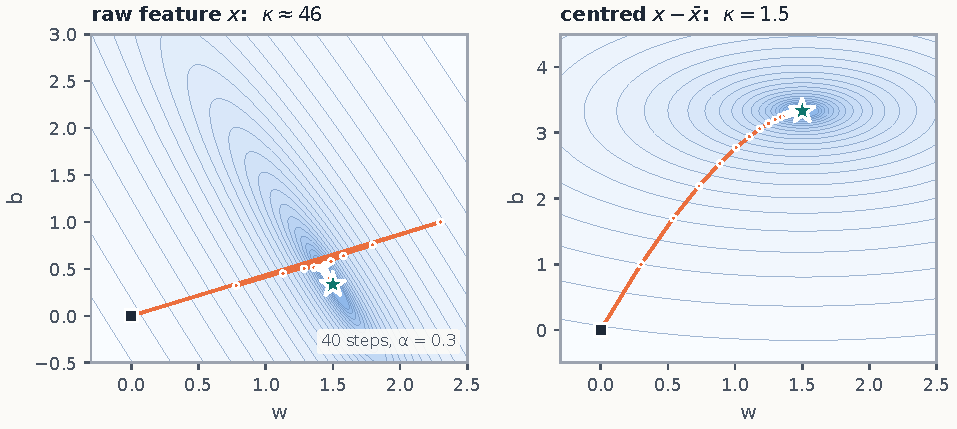
\includegraphics[width=0.54\textwidth]{fig_scaling}
\end{frame}

\begin{frame}{\soltitle{A1}{4}{4}}
  \textbf{(d) The optimum.} Setting $\nabla\mathcal L = \mathbf 0$ gives the normal equations
  (using $\sum x_i = 6$, $\sum x_i^2 = 14$, $\sum y_i = 10$, $\sum x_iy_i = 23$):
  \[
    14w + 6b = 23,\qquad 6w + 3b = 10
    \;\Longrightarrow\; \ans{w = 1.5,\;\; b = \tfrac13}, \qquad \mathcal L^\star = \tfrac1{36} \approx 0.0278 .
  \]
  The centred model gives $\hat y = 1.5(x-2) + \tfrac{10}{3}$, which is \emph{the same line}. Centring changes
  the shape of the optimisation problem, not its answer.

  \vspace{4pt}
  \begin{keybox}[The bigger picture]
    \small
    \begin{itemize}
      \item Centring and standardising features is a change of variables that acts as a \emph{preconditioner}:
            GD sees nearly round contours instead of a narrow valley.
      \item Here a closed form exists. With millions of parameters there is none, GD or SGD is the only practical
            solver, and conditioning decides how long training takes.
    \end{itemize}
  \end{keybox}
\end{frame}

% =====================================================================
%  A2 -- Structural mechanics: spring-chain equilibrium
% =====================================================================
\subsection{A2: Structural mechanics, a spring chain at rest}
\setprob{A2}

\begin{frame}{\probtitle{A2}{Where does a spring chain settle? Energy minimisation}}
  \begin{probbox}[Problem A2 \hfill Application: Structural Mechanics \quad $\star\star$]
    \begin{columns}[T]
      \begin{column}{0.47\textwidth}
        \centering
        % Spring chain for Problem A2: wall -- k1 -- m1 -- k2 -- m2 <- F
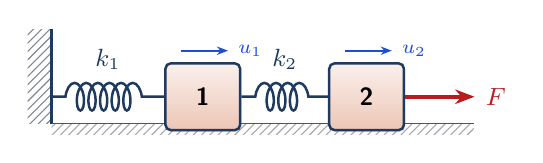
\begin{tikzpicture}[scale=0.8, every node/.style={font=\small},
  spring/.style={decorate, decoration={coil, aspect=0.45, segment length=4.2pt, amplitude=5pt,
                 pre length=5pt, post length=5pt}, line width=0.9pt, mDarkTeal},
  mass/.style={draw=mDarkTeal, line width=0.9pt, top color=mOrange!8, bottom color=mOrange!30,
               minimum width=0.95cm, minimum height=0.85cm, rounded corners=2pt,
               drop shadow={opacity=0.18, shadow xshift=0.5pt, shadow yshift=-0.7pt}}]
  % ground and wall
  \fill[pattern=north east lines, pattern color=mGrey!70] (-0.38,-0.75) rectangle (0,0.75);
  \draw[line width=1.2pt, mDarkTeal] (0,-0.75) -- (0,0.75);
  \fill[pattern=north east lines, pattern color=mGrey!50] (0,-0.75) rectangle (6.7,-0.92);
  \draw[mGrey] (0,-0.75) -- (6.7,-0.75);
  % masses
  \node[mass] (m1) at (2.4,-0.32) {\textbf{1}};
  \node[mass] (m2) at (5.0,-0.32) {\textbf{2}};
  % springs
  \draw[spring] (0,-0.32) -- node[above=6pt] {$k_1$} (m1.west);
  \draw[spring] (m1.east) -- node[above=6pt] {$k_2$} (m2.west);
  % load
  \draw[-{Stealth[length=7pt]}, line width=1.6pt, mRed] (m2.east) -- ++(1.1,0) node[right] {$F$};
  % displacements
  \draw[-{Stealth[length=4pt]}, line width=0.8pt, mBlue] ($(m1.north)+(-0.35,0.18)$) -- ++(0.75,0) node[right, font=\scriptsize] {$u_1$};
  \draw[-{Stealth[length=4pt]}, line width=0.8pt, mBlue] ($(m2.north)+(-0.35,0.18)$) -- ++(0.75,0) node[right, font=\scriptsize] {$u_2$};
\end{tikzpicture}

      \end{column}
      \begin{column}{0.5\textwidth}
        \small
        Two masses are joined by springs and a load $F$ pulls on mass 2. The chain comes to rest where the
        potential energy is smallest:
        \[
          \Pi(\vu) = \tfrac12k_1u_1^2 + \tfrac12k_2(u_2-u_1)^2 - Fu_2 .
        \]
      \end{column}
    \end{columns}
    \vspace{-2pt}
    \begin{enumerate}[(a)]
      \item Write $\Pi = \tfrac12\vu\T\bK\vu - \vf\T\vu$ and show that $\nabla\Pi = \mathbf 0$ is force balance.
      \item With $k_1 = 3$, $k_2 = 1$ kN/mm and $F = 1$ kN, find $\vu^\star$, $\operatorname{eig}(\bK)$, $\kappa$, the stable range of $\alpha$,
            the best $\alpha$ and its rate.
      \item Take two GD iterations from $\vu_0 = \mathbf 0$ with $\alpha = 0.4$.
      \item Make the support very stiff, $k_1 = 1000$. What changes, and why is this a \emph{stiff} problem?
    \end{enumerate}
  \end{probbox}
\end{frame}

\begin{frame}{\soltitle{A2}{1}{4}}
  \textbf{(a)} Expand $\tfrac12k_2(u_2^2 - 2u_1u_2 + u_1^2)$ to read off
  \[
    \bK = \begin{pmatrix}k_1+k_2 & -k_2\\ -k_2 & k_2\end{pmatrix}, \qquad
    \vf = \begin{pmatrix}0\\ F\end{pmatrix}, \qquad
    \nabla\Pi = \bK\vu - \vf .
  \]
  Setting each component to zero:
  \begin{align*}
    (k_1+k_2)u_1 - k_2u_2 = 0 &\iff k_1u_1 = k_2(u_2-u_1) \quad\text{(balance at mass 1)}\\
    k_2(u_2 - u_1) = F &\iff \text{spring 2 carries the load} \quad\text{(balance at mass 2)}
  \end{align*}
  \begin{keybox}[What GD is doing physically]
    $-\nabla\Pi = \vf - \bK\vu$ is the \alert{unbalanced force} on each mass, and GD nudges each mass along it:
    relaxation in pseudo-time. Since $\bK\succ0$, there is exactly one resting position.
  \end{keybox}
\end{frame}

\begin{frame}{\soltitle{A2}{2}{4}}
  \textbf{(b)} $\bK = \begin{pmatrix}4&-1\\-1&1\end{pmatrix}$ and $\det\bK = 3$:
  \[
    \vu^\star = \bK^{-1}\vf = \frac13\begin{pmatrix}1&1\\1&4\end{pmatrix}\begin{pmatrix}0\\1\end{pmatrix}
    = \ans{\bigl(\tfrac13,\ \tfrac43\bigr)\ \text{mm}}
  \]
  Sanity check with springs in series: $u_1 = F/k_1 = \tfrac13$ and $\;u_2 = u_1 + F/k_2 = \tfrac43$ \checkmark.

  \vspace{2pt}
  $\lambda^2 - 5\lambda + 3 = 0 \Rightarrow \lambda = \tfrac{5\mp\sqrt{13}}{2} = 0.6972,\ 4.3028$, so $\ans{\kappa = 6.17}$.
  \[
    0 < \alpha < \frac{2}{4.3028} = \ans{0.4648},\qquad
    \alpha^\star = \frac{2}{\lambda_1+\lambda_2} = \ans{0.4},\qquad
    \rho = \frac{\sqrt{13}}{5} = \ans{0.7211}.
  \]
  Getting to $10^{-6}$ accuracy takes $\lceil\ln10^6/\ln(1/0.7211)\rceil = 43$ iterations.
\end{frame}

\begin{frame}{\soltitle{A2}{3}{4}}
  \textbf{(c) Two iterations} with $\alpha = 0.4$ and $\g_k = \bK\vu_k - \vf$:

  \vspace{2pt}
  \centering
  \begin{tabular}{@{}c c c c@{}}
    \toprule
    $k$ & $\vu_k$ (mm) & $\g_k$ & $\Pi(\vu_k)$ \\
    \midrule
    0 & $(0,\ 0)$ & $(0,\ -1)$ & $0$ \\
    1 & $(0,\ 0.4)$ & $(-0.4,\ -0.6)$ & $-0.3200$ \\
    2 & $\ans{(0.16,\ 0.64)}$ & $(0,\ -0.52)$ & $-0.4864$ \\
    $\star$ & $(0.3333,\ 1.3333)$ & $(0,\ 0)$ & $-0.6667$ \\
    \bottomrule
  \end{tabular}

  \raggedright
  \begin{keybox}[Insight: news travels one spring per iteration]
    After step 1 only mass 2 has moved; mass 1 ``hears'' about the load at step 2. Since
    $\vu_k \in \operatorname{span}\{\vf,\bK\vf,\dots,\bK^{k-1}\vf\}$ and $\bK$ is tridiagonal, a chain of $N$ springs
    needs at least $N$ iterations before every mass has moved.
  \end{keybox}
\end{frame}

\begin{frame}{\soltitle{A2}{4}{4}}
  \textbf{(d) A stiff support, $k_1 = 1000$:} $\;\bK = \begin{pmatrix}1001 & -1\\ -1 & 1\end{pmatrix}$.
  \vspace{-4pt}
  \[
    \lambda \approx 0.999,\ 1001.001 \;\Rightarrow\; \ans{\kappa \approx 1002},\qquad
    \alpha_{\max} \approx 0.0020,\qquad \rho \approx 0.998 .
  \]
  \vspace{-6pt}
  Iterations for $10^{-6}$: \alert{about 6922} instead of 43, for the easy answer $\vu^\star = (0.001,\ 1.001)$ mm.
  \begin{itemize}\footnotesize
    \item The stiff spring forces a tiny $\alpha$ for stability, and then the soft mode crawls. GD is explicit Euler on
          $\dot\vu = -(\bK\vu - \vf)$, whose eigenvalues span three orders of magnitude. That is a textbook \alert{stiff ODE}.
    \item \textbf{The fix is Jacobi scaling:} $\mathbf D^{-1/2}\bK\mathbf D^{-1/2}$ with $\mathbf D = \diag(\bK)$ has
          eigenvalues $1\pm\tfrac1{\sqrt{1001}}$, so $\kappa \approx 1.065$.
  \end{itemize}
  \begin{keybox}[Engineering lesson]
    Stiff members next to soft ones make the landscape ill-conditioned: rescale before using a first-order solver.
  \end{keybox}
\end{frame}

% =====================================================================
%  A3 -- Economics: two-product profit maximisation
% =====================================================================
\subsection{A3: Economics, two-product profit maximisation}
\setprob{A3}

\begin{frame}{\probtitle{A3}{Maximising a two-product profit by gradient ascent}}
  \begin{probbox}[Problem A3 \hfill Application: Economics \quad $\star\star$]
    A firm sells two substitute products in quantities $x$ and $y$ (hundreds of units). Its profit,
    in thousand Tk, is
    \[
      P(x,y) = 100x + 80y - 2x^2 - 2y^2 - 2xy .
    \]
    Each period the firm adjusts production by \emph{gradient ascent}, $\x_{k+1} = \x_k + \alpha\nabla P(\x_k)$.
    \begin{enumerate}[(a)]
      \item Find the optimum analytically and show that it is a global maximum.
      \item Find the stable range of $\alpha$ and the best fixed $\alpha$.
      \item Run three iterations from $(0,0)$ with the best $\alpha$, and tabulate $P$ and the error.
      \item Explain what $\alpha = 0.4$ does, in business terms.
    \end{enumerate}
  \end{probbox}
  \footnotesize\textcolor{mGrey}{The point: ascent is just descent on $-P$, and a hand calculation matches the theory exactly.}
\end{frame}

\begin{frame}{\soltitle{A3}{1}{3}}
  \textbf{(a)}
  $\nabla P = \begin{pmatrix}100 - 4x - 2y\\ 80 - 2x - 4y\end{pmatrix} = \mathbf 0
  \iff \begin{cases}4x + 2y = 100\\ 2x + 4y = 80\end{cases}
  \iff \ans{(x^\star,y^\star) = (20,\ 10)}$
  \[
    \nabla^2P = \begin{pmatrix}-4&-2\\-2&-4\end{pmatrix}, \quad \text{eigenvalues } -2,\,-6
    \;\Rightarrow\; \text{negative definite} \;\Rightarrow\; \text{global maximum}
  \]
  \[
    P^\star = 2000 + 800 - 800 - 200 - 400 = \ans{1400} \text{ thousand Tk}.
  \]
  \textbf{(b)} Ascent on $P$ is GD on $-P$, with $\bA = \begin{pmatrix}4&2\\2&4\end{pmatrix}$:
  $\lambda = 2$ along $(1,-1)$ and $\lambda = 6$ along $(1,1)$.
  \[
    \ans{0 < \alpha < \tfrac26 = \tfrac13},\qquad
    \alpha^\star = \tfrac{2}{2+6} = \ans{\tfrac14},\qquad
    \rho = \tfrac{6-2}{6+2} = \ans{\tfrac12}.
  \]
\end{frame}

\begin{frame}{\soltitle{A3}{2}{3}}
  \begin{columns}[T]
    \begin{column}{0.56\textwidth}
      \textbf{(c)} $\alpha = \tfrac14$, starting from $(0,0)$:

      \vspace{2pt}
      \footnotesize
      \begin{tabular}{@{}c c c c c@{}}
        \toprule
        $k$ & $\x_k$ & $\nabla P(\x_k)$ & $P$ & $\norm{\e_k}$\\
        \midrule
        0 & $(0,0)$ & $(100,80)$ & $0$ & $22.361$\\
        1 & $(25,20)$ & $(-40,-50)$ & $1050$ & $11.180$\\
        2 & $(15,7.5)$ & $(25,20)$ & $1312.5$ & $5.590$\\
        3 & $(21.25,12.5)$ & $(-10,-12.5)$ & $1378.125$ & $2.795$\\
        \bottomrule
      \end{tabular}

      \vspace{4pt}
      \small
      \begin{itemize}
        \item The error \alert{halves exactly} every step, because both factors, $1 - \tfrac14\cdot2 = \tfrac12$ and
              $1 - \tfrac14\cdot6 = -\tfrac12$, have size $\tfrac12$.
        \item The profit gap shrinks by $\rho^2 = \tfrac14$ per step: $1400 \to 350 \to 87.5 \to 21.875$.
      \end{itemize}
    \end{column}
    \begin{column}{0.42\textwidth}
      \centering
      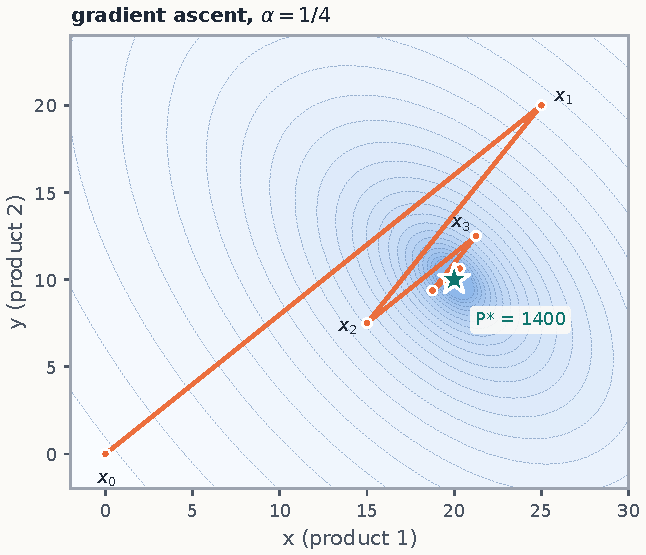
\includegraphics[width=0.95\linewidth]{fig_profit}
    \end{column}
  \end{columns}
\end{frame}

\begin{frame}{\soltitle{A3}{3}{3}}
  \textbf{The overshoot pattern.} The $(1,1)$ part of the error changes sign every step (its factor is $-\tfrac12$).
  So total production first \emph{overshoots} ($25+20 = 45 > 30$), then \emph{undershoots}, then overshoots again,
  by half as much each time.

  \smallskip
  \textbf{(d) $\alpha = 0.4 > \tfrac13$.} Now the factor along $(1,1)$ is $1 - 0.4\cdot6 = \alert{-1.4}$, and
  $\x_6 \approx (-92.9,\ -102.9)$. The swings grow instead of dying out.
  \smallskip
  In business terms: a management that \emph{over-reacts} to the marginal-profit signal pushes total output
  further from the optimum every period, until it is planning negative (meaningless) quantities.
  \begin{keybox}[Lesson]
    How fast you adjust has to respect the curvature of the profit function: $\alpha < 2/\lmax$.
    Because the goods are substitutes (the $-2xy$ term), $\lmax$ rises from $4$ to $6$ and the safe step gets smaller.
  \end{keybox}
\end{frame}

% =====================================================================
%  A4 -- Parameter estimation: Newton's law of cooling
% =====================================================================
\subsection{A4: Parameter estimation, Newton's law of cooling}
\setprob{A4}

\begin{frame}{\probtitle{A4}{Estimating a cooling constant by nonlinear least squares}}
  \begin{probbox}[Problem A4 \hfill Application: Parameter Estimation \quad $\star\star\star$]
    By Newton's law of cooling, the normalised temperature $\theta = \frac{T - T_a}{T_0 - T_a}$ follows
    $\theta(t) = e^{-kt}$. We measure $\theta(1) = 0.60$ and $\theta(2) = 0.36$ ($t$ in minutes) and estimate $k$ by minimising
    \[
      J(k) = \tfrac12\sum_{i=1}^{2}\bigl(e^{-kt_i} - \theta_i\bigr)^2 .
    \]
    \vspace{-8pt}
    \begin{enumerate}[(a)]
      \item Derive $J'(k)$ and $J''(k)$, and find the exact minimiser $k^\star$.
      \item Run two GD iterations from $k_0 = 0$ with $\alpha = 0.5$. Does GD converge?
      \item Compare the curvature $J''$ at $k = 0$ and at $k^\star$. Where is $J$ convex?
      \item Now start from a poor guess, $k_0 = 6$. What does GD do, and how would you fix it?
    \end{enumerate}
  \end{probbox}
  \footnotesize\textcolor{mGrey}{The point: a nonconvex fit, curvature that varies, and the plateau failure mode.}
\end{frame}

\begin{frame}{\soltitle{A4}{1}{4}}
  \textbf{(a)} With residuals $r_i(k) = e^{-kt_i} - \theta_i$,
  \[
    J'(k) = -\sum_i r_i\,t_i\,e^{-kt_i}, \qquad
    J''(k) = \underbrace{\sum_i t_i^2 e^{-2kt_i}}_{\text{Gauss--Newton part} \ \ge 0}
           + \underbrace{\sum_i r_i\,t_i^2 e^{-kt_i}}_{\text{residual part (either sign)}}.
  \]
  The data fit the model perfectly: $e^{-k} = 0.6$ and $e^{-2k} = 0.36 = 0.6^2$. So $J(k^\star) = 0$ at
  \[
    \ans{k^\star = \ln\tfrac53 \approx 0.5108\ \text{min}^{-1}}.
  \]
  \vspace{-4pt}
  \begin{keybox}[Why this is not a linear problem]
    $J$ depends on $k$ through $e^{-kt}$, so it is \emph{not} quadratic. Its curvature changes with $k$,
    which means there is no longer one step size that is safe everywhere.
  \end{keybox}
\end{frame}

\begin{frame}{\soltitle{A4}{2}{4}}
  \textbf{(b) Two GD iterations} with $\alpha = 0.5$:
  \begin{itemize}\small
    \item $k_0 = 0$: $\;r = (0.4,\ 0.64)$, $\;J'(0) = -(0.4\cdot1 + 0.64\cdot2) = -1.68$,
          so $k_1 = 0 + 0.5(1.68) = \ans{0.84}$.
    \item $k_1 = 0.84$: $\;e^{-0.84} = 0.43171$, $\;e^{-1.68} = 0.18637$, $\;r = (-0.16829,\ -0.17363)$, and
          \[
            J'(0.84) = -\bigl[(-0.16829)(1)(0.43171) + (-0.17363)(2)(0.18637)\bigr] = 0.13737
          \]
          so $k_2 = 0.84 - 0.5(0.13737) = \ans{0.7713}$.
  \end{itemize}
  \[
    J:\quad 0.2848 \;\to\; 0.02923 \;\to\; 0.02015 \quad(\text{going down})
  \]
  The steep gradient at $k = 0$ makes the first step \alert{overshoot} $k^\star$; after that the iterates come back from above.
  GD reaches $k^\star = 0.510826$ to within $10^{-6}$ in \ans{26} iterations.
\end{frame}

\begin{frame}{\soltitle{A4}{3}{4}}
  \textbf{(c) Curvature.}\quad
  $J''(0) = (1 + 0.4) + (4 + 4\cdot0.64) = \ans{7.96}$, \qquad
  $J''(k^\star) = 0.36 + 4(0.1296) = \ans{0.8784}$ \;(the residuals vanish there).

  \vspace{2pt}
  \centering
  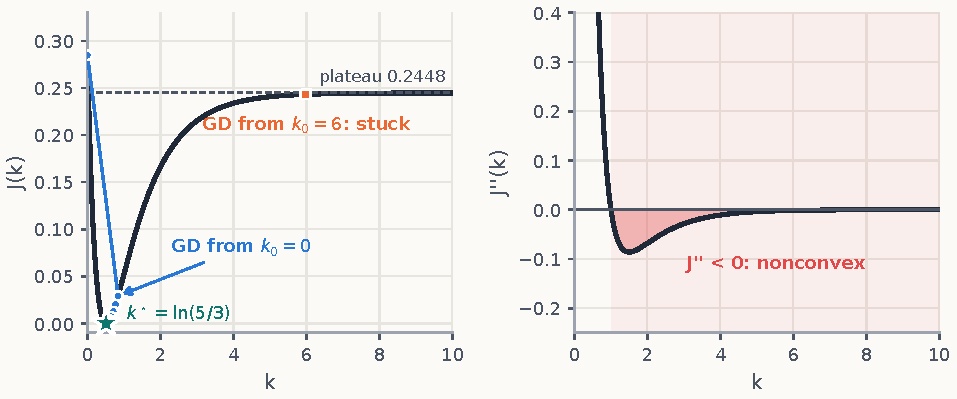
\includegraphics[width=0.52\textwidth]{fig_cooling_loss}

  \raggedright\small
  \begin{itemize}
    \item The local stability limit $2/J''$ is $0.25$ at $k = 0$ but $2.28$ at $k^\star$, a ninefold change.
          Near $k^\star$ the rate is $|1 - 0.5(0.8784)| = 0.56$ per step.
    \item For $k \gtrsim 1.00$ (shaded) $J'' < 0$, so $J$ is \alert{nonconvex} there and no global step-size result applies.
  \end{itemize}
\end{frame}

\begin{frame}{\soltitle{A4}{4}{4}}
  \textbf{(d) A bad start, $k_0 = 6$.} Here $e^{-6} = 0.00248$ and $e^{-12} \approx 6\times10^{-6}$, so the model says
  the object is ``already cold'' at both measurement times:
  \[
    J(6) = 0.2433 \approx \tfrac12\textstyle\sum\theta_i^2 = 0.2448 \;(\text{plateau}),\qquad
    J'(6) \approx 1.5\times10^{-3}.
  \]
  Each step moves $k$ by only about $7\times10^{-4}$. After \alert{1000 iterations} we are at $k \approx 4.65$.
  GD has \alert{stalled on a plateau}: the gradient vanishes because the model has saturated.

  \vspace{4pt}
  \begin{keybox}[How to get unstuck]
    \small
    \begin{itemize}
      \item \textbf{Start somewhere sensible.} Linearising, $\ln\theta = -kt$ gives $k \approx -\ln 0.6 = 0.51$.
      \item \textbf{Reparametrise}, e.g.\ $k = e^{s}$, or fit $\ln\theta$ instead, which reshapes the landscape.
      \item \textbf{Adapt the step} with a line search or curvature scaling, so it does not stay tiny on flat ground.
    \end{itemize}
  \end{keybox}
\end{frame}

% =====================================================================
%  A5 -- Signal processing: streaming sensor calibration by SGD
% =====================================================================
\subsection{A5: Signal processing, calibrating a sensor with SGD}
\setprob{A5}

\begin{frame}{\probtitle{A5}{Calibrating a streaming sensor with SGD}}
  \begin{probbox}[Problem A5 \hfill Application: Signal Processing \quad $\star\star$]
    A temperature sensor reports $\xi_k = \theta + \varepsilon_k$, where the $\varepsilon_k$ are i.i.d.\ with mean $0$ and variance $\sigma^2 = 0.25\ (^\circ\text{C})^2$.
    We estimate $\theta$ by minimising $F(x) = \tfrac12\E\bigl[(x-\xi)^2\bigr]$, using \emph{one new reading per step}:
    \[
      x_{k+1} = x_k - \alpha_k\,(x_k - \xi_{k+1}) \qquad\text{(stochastic gradient descent)}.
    \]
    \vspace{-10pt}
    \begin{enumerate}[(a)]
      \item Show that $\nabla F(x) = x - \theta$ and that the stochastic gradient $x - \xi$ is unbiased.
      \item Show that $\alpha_k = \tfrac1{k+1}$ with $x_1 = \xi_1$ gives the running sample mean, so $\operatorname{Var}(x_k) = \sigma^2/k$.
      \item For a constant $\alpha$, show that $\operatorname{Var}(x_k) \to \alpha\sigma^2/(2-\alpha)$.
      \item With readings $20.4,\ 19.7,\ 20.2,\ 20.6,\ 19.9$, run both schedules (constant $\alpha = 0.5$).
      \item Connect the results to the Robbins--Monro step-size conditions.
    \end{enumerate}
  \end{probbox}
\end{frame}

\begin{frame}{\soltitle{A5}{1}{5}}
  \textbf{(a)} Expand, using $\E\xi = \theta$ and $\operatorname{Var}\xi = \sigma^2$:
  \[
    F(x) = \tfrac12\E\bigl[(x - \theta - \varepsilon)^2\bigr] = \tfrac12(x-\theta)^2 + \tfrac12\sigma^2
    \;\Longrightarrow\; \ans{\nabla F(x) = x - \theta}, \quad x^\star = \theta .
  \]
  So $F$ is a quadratic with $\mu = L = 1$. The stochastic gradient $G(x,\xi) = x - \xi$ has
  $\E[G] = x - \theta = \nabla F(x)$: it is \alert{unbiased}, and it needs only one reading instead of the whole expectation.

  \vspace{4pt}
  \textbf{(b) Induction.} Suppose $x_k = \frac1k\sum_{i\le k}\xi_i$. Then
  \[
    x_{k+1} = x_k + \frac{\xi_{k+1} - x_k}{k+1} = \frac{k\,x_k + \xi_{k+1}}{k+1}
    = \frac{1}{k+1}\sum_{i\le k+1}\xi_i . \qquad\blacksquare
  \]
  The readings are independent, so $\operatorname{Var}(x_k) = \ans{\sigma^2/k} \to 0$. With this schedule SGD \emph{is} the sample mean.
\end{frame}

\begin{frame}{\soltitle{A5}{2}{5}}
  \textbf{(c) Constant step.} Subtract $\theta$ from both sides:
  \[
    x_{k+1} - \theta = (1-\alpha)(x_k - \theta) + \alpha\,\varepsilon_{k+1}.
  \]
  \begin{itemize}\small
    \item \textbf{Mean:} $\E[x_k] - \theta = (1-\alpha)^k(x_0 - \theta) \to 0$ geometrically, so the bias disappears.
    \item \textbf{Variance:} $\varepsilon_{k+1}$ is independent of $x_k$, so
          $V_{k+1} = (1-\alpha)^2V_k + \alpha^2\sigma^2$. Its fixed point is
  \end{itemize}
  \[
    V_\infty = \frac{\alpha^2\sigma^2}{1-(1-\alpha)^2} = \frac{\alpha^2\sigma^2}{\alpha(2-\alpha)}
    = \ans{\frac{\alpha\sigma^2}{2-\alpha}} \qquad (0<\alpha<2).
  \]
  \begin{keybox}[The noise ball]
    Constant-step SGD gets close fast, then jitters in a \emph{neighbourhood} of radius $O(\sqrt\alpha)$.
    Monte-Carlo, $\alpha = 0.1$: $V_\infty = 0.01320$ against $0.01316$ predicted.
  \end{keybox}
\end{frame}

\begin{frame}{\soltitle{A5}{3}{5}}
  \begin{columns}[T]
    \begin{column}{0.42\textwidth}
      \textbf{(d)} Both schedules start from $x_1 = \xi_1 = 20.4$:

      \vspace{3pt}
      \footnotesize
      \begin{tabular}{@{}c c c c@{}}
        \toprule
        $k$ & $\xi_k$ & $\alpha_k = \frac1{k+1}$ & $\alpha = 0.5$\\
        \midrule
        1 & 20.4 & 20.4000 & 20.4000\\
        2 & 19.7 & 20.0500 & 20.0500\\
        3 & 20.2 & 20.1000 & 20.1250\\
        4 & 20.6 & 20.2250 & 20.3625\\
        5 & 19.9 & \ans{20.1600} & \ans{20.1313}\\
        \bottomrule
      \end{tabular}

      \vspace{4pt}
      \small
      Standard deviations: the sample mean after 5 readings has $\sqrt{0.25/5} = 0.224$ and it keeps shrinking;
      $\alpha = 0.5$ is stuck at $\sqrt{0.5\cdot0.25/1.5} = 0.289$.
    \end{column}
    \begin{column}{0.56\textwidth}
      \centering
      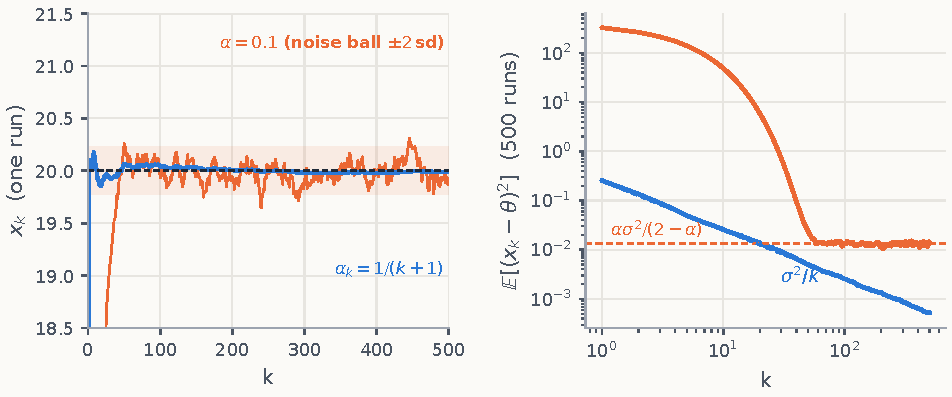
\includegraphics[width=\linewidth]{fig_sgd}

      \vspace{2pt}
      \footnotesize A constant step weights old readings by $\alpha(1-\alpha)^j$, so it slowly forgets them.
      That is useful if $\theta$ drifts, and wasteful if it does not.
    \end{column}
  \end{columns}
\end{frame}

\begin{frame}{\soltitle{A5}{4}{5}}
  \textbf{(e) The Robbins--Monro conditions:}
  \[
    \sum_k\alpha_k = \infty \qquad\text{and}\qquad \sum_k\alpha_k^2 < \infty .
  \]
  \begin{itemize}\small
    \item $\sum\alpha_k = \infty$: the steps add up to enough ``travel'' to forget the start, since $\prod(1-\alpha_k)\to0$.
    \item $\sum\alpha_k^2 < \infty$: the total injected noise variance $\sum\alpha_k^2\sigma^2$ stays finite and gets averaged away.
  \end{itemize}
  \vspace{2pt}
  \centering\small
  \begin{tabular}{@{}l c c l@{}}
    \toprule
    Schedule ($k\ge1$) & $\sum\alpha_k$ & $\sum\alpha_k^2$ & What happens \\
    \midrule
    $\alpha_k = \frac1{k+1}$ & $\infty$ & $\frac{\pi^2}{6} - 1$ & converges to $\theta$ \checkmark \\
    $\alpha_k = \alpha$ & $\infty$ & $\infty$ & noise ball, $V_\infty = \frac{\alpha\sigma^2}{2-\alpha}$ \\
    $\alpha_k = \frac{1}{(k+1)^2}$ & $< \infty$ & $< \infty$ & stops moving too early \\
    \bottomrule
  \end{tabular}

  \raggedright\small
  For $\frac1{(k+1)^2}$, $\prod_{k\ge1}\bigl(1-\frac1{(k+1)^2}\bigr) = \frac12$: only half of any initial error ever gets removed.
\end{frame}

\begin{frame}{\soltitle{A5}{5}{5}}
  \textbf{Beyond this example.}
  \begin{itemize}\small
    \item \textbf{Mini-batches:} averaging $B$ readings per step divides the noise variance by $B$:
          \[
            V_\infty = \frac{\alpha\sigma^2}{B\,(2-\alpha)} .
          \]
          This is the step-size against batch-size trade-off behind large-scale machine learning.
    \item \textbf{Any strongly convex $F$:} with a fixed step, the expected optimality gap of SGD falls linearly
          to a floor proportional to $\alpha$. With diminishing steps $\alpha_k = O(1/k)$ it decays like
          $O(1/k)$~\cite{bottou2018}.
  \end{itemize}
  \begin{keybox}[Takeaway]
    A decaying schedule gives up speed to gain accuracy. A constant step gives up accuracy to gain speed and the
    ability to follow changes. Practical schedules (constant first, then decaying) get some of both.
  \end{keybox}
\end{frame}


% ---------------- Back matter ---------------------------------------
\setprob{}
\section{References}
\begin{frame}[allowframebreaks]{References}
  \scriptsize
  \nocite{chapra,bubeck2015}
  \bibliographystyle{plain}
  \bibliography{bibliography/references}
\end{frame}

\end{document}
